\documentclass[11pt]{article}

\usepackage[a4paper, margin=2cm,headsep=6pt]{geometry}
\usepackage{lineno}
\usepackage[utf8]{inputenc}
\usepackage[english]{babel}
\usepackage{graphicx}
\usepackage{amsmath}
\usepackage{multirow}
\usepackage{caption}
\usepackage{array}
\usepackage{float}
\usepackage{csvsimple}
\usepackage{rotating}
\usepackage{lscape}
\usepackage{adjustbox}
\newcolumntype{P}[1]{>{\centering\arraybackslash}p{#1}}
\newcommand{\soptitle}{Modelling the read depth of next generation sequencing data}
\usepackage{fancyhdr}
\pagestyle{fancy}
\linespread{1.25}
\fancyhead[R]{CID 01383312}
\fancyhead[L]{Oliver Tarrant}
\usepackage{csquotes}
\usepackage[backend=bibtex,style=authoryear]{biblatex}

\begin{filecontents*}{poissondata.csv}
Sample,Curves,AIC,Mu1,Mu2,Mu3,Mu4,Mu5,Coef1,Coef2,Coef3,Coef4,Coef5
Sample1,5,-1516.004,28.8510254,48.1490036,68.1803503,89.0569604,112.156653,0.07050601,0.13072499,0.2263166,0.31545774,0.25699466
Sample2,4,-1013.964,78.6182099,93.5148646,107.202179,125.508445,0.0,0.10897253,0.21804332,0.36484128,0.30814287,0.0
Sample3,3,-448.317,21.9629541,33.5192306,41.9525858,0.0,0.0,0.08165849,0.37283083,0.54551068,0.0,0.0
Sample4,2,-567.715,44.6792956,58.5066163,0.0,0.0,0.0,0.15470747,0.84529253,0.0,0.0,0.0
Sample5,5,-1666.361,30.8756043,49.2020619,72.488984,99.6975078,129.117617,0.17078384,0.18023886,0.19372999,0.23313912,0.22210819
Sample6,4,-913.641,44.3306436,58.7001289,72.7464768,89.5417493,0.0,0.10973124,0.25769961,0.37303643,0.25953272,0.0
Sample7,5,-627.898,1.86404566,8.30979917,30.6825168,20.3949643,40.8207556,0.02586037,0.02441112,0.3655169,0.07725494,0.50695667
Sample8,3,-471.281,23.6335183,33.2626484,45.7047584,0.0,0.0,0.27736913,0.44771069,0.27492018,0.0,0.0
Sample9,3,-798.214,68.5230219,84.6087402,102.131152,0.0,0.0,0.20131126,0.43826352,0.36042522,0.0,0.0
Sample10,4,-1378.076,114.589073,135.306047,152.22053,177.489141,0.0,0.12819608,0.40433944,0.32070124,0.14676324,0.0
Sample11,5,-1262.877,20.8077397,34.3988858,51.5176825,71.8571708,94.5776707,0.15757149,0.17872661,0.20051644,0.23435033,0.22883513
Sample12,4,-508.635,12.5626284,20.1206113,28.3346701,39.1925325,0.0,0.09366934,0.27523421,0.37884514,0.25225131,0.0
Sample13,4,-833.73,55.9000021,67.2139412,78.1154987,95.9135852,0.0,0.17261296,0.29243813,0.31399979,0.22094912,0.0
Sample14,3,-540.579,37.3438451,48.1486344,62.150612,0.0,0.0,0.26232701,0.43129975,0.30637324,0.0,0.0
Sample15,4,-859.043,61.1055834,73.9438335,85.6087644,101.935791,0.0,0.12555094,0.22178445,0.34494356,0.30772105,0.0
Sample16,5,-765.031,11.1635651,18.41939,27.3365212,39.149506,54.5132028,0.14386123,0.27622711,0.24826363,0.17911136,0.15253667
Sample17,4,-1094.25,70.239065,86.1849832,47.0335853,101.652516,0.0,0.08116605,0.40909042,0.01928062,0.49046291,0.0
Sample18,5,-886.621,1.92791026,46.1281238,9.52548145,24.5070063,55.6979416,0.01902987,0.30248155,0.0184497,0.01973115,0.64030773
Sample19,3,-691.442,45.2549861,58.7095844,75.4218347,0.0,0.0,0.26674592,0.44221571,0.29103837,0.0,0.0
Sample20,5,-1184.807,25.8297678,39.7212454,56.0896172,74.046233,93.4007601,0.11673517,0.14114245,0.18759294,0.27423364,0.2802958
Sample21,5,-1228.034,36.8520502,52.048791,66.3312128,82.2581947,99.7250112,0.03867444,0.12777238,0.2238604,0.33956326,0.27012952
Sample22,4,-719.1,38.9359536,49.517866,59.8959509,74.7015532,0.0,0.17342985,0.26808543,0.31336137,0.24512335,0.0
\end{filecontents*}
\begin{filecontents*}{negativebinomialdata.csv}
Sample,Curves,AIC,Mu1,Mu2,Mu3,Mu4,Mu5,Coef1,Coef2,Coef3,Coef4,Coef5
Sample1,5,-1505.911,29.10483,48.430032,68.480505,89.2598929,112.3209,0.07120109,0.13178801,0.22719011,0.31462932,0.25519147
Sample2,4,-998.468,81.986323,99.415274,107.51112298,124.8216107,0.0,0.16794608,0.25921528,0.24037899,0.33245965,0.0
Sample3,3,-441.994,22.330447,33.9696689,42.2319398,0.0,0.0,0.08658493,0.39667904,0.51673603,0.0,0.0
Sample4,2,-563.689,44.551144,58.5056839,0.0,0.0,0.0,0.15252041,0.84747959,0.0,0.0,0.0
Sample5,5,-1656.331,30.991914,49.346088,72.730255,99.8815977,129.298249,0.17134138,0.18054884,0.19389609,0.23300156,0.22121213
Sample6,4,-905.522,44.41094,58.90119297,73.023849365,89.776218,0.0,0.11130912,0.26121194,0.37227933,0.25519961,0.0
Sample7,5,-617.758,1.922276,8.68751,20.76682458,30.866227,40.913326,0.02624816,0.02483309,0.08098601,0.36723153,0.50070121
Sample8,3,-465.273,23.66517,33.259899,45.7530694,0.0,0.0,0.2769791,0.44807936,0.27494154,0.0,0.0
Sample9,3,-791.464,68.49856,84.956165,102.51880468,0.0,0.0,0.20215914,0.44834473,0.34949613,0.0,0.0
Sample10,4,-1369.621,113.98665,134.8972678,151.95971616,177.28162,0.0,0.1221878,0.3998234,0.33038714,0.14760166,0.0
Sample11,5,-1252.878,20.827334,34.388499,51.52486084,71.839781,94.560756,0.15744545,0.17889523,0.20038919,0.23424152,0.22902861
Sample12,4,-500.583,12.529975,20.033429,28.230944115,39.0942323,0.0,0.09265858,0.27131513,0.38028737,0.25573892,0.0
Sample13,4,-825.411,56.40973,67.913306,78.558505556,96.234319,0.0,0.18674936,0.29389109,0.30277809,0.21658146,0.0
Sample14,3,-534.568,37.42922,48.2393455,62.24925368,0.0,0.0,0.26430765,0.43140813,0.30428422,0.0,0.0
Sample15,3,-848.29,64.06332,81.7447038,100.729312548,0.0,0.0,0.19733727,0.44428751,0.35837522,0.0,0.0
Sample16,5,-755.01,11.139171,18.4050807,27.335088595,39.1620486,54.53491,0.14269765,0.27670442,0.24911718,0.17910613,0.15237462
Sample17,3,-1068.835,66.80022,85.506239,101.61150937,0.0,0.0,0.07092194,0.42166761,0.50741045,0.0,0.0
Sample18,5,-875.907,2.0429798,26.7095379,10.4708551341,55.8461098,46.443287,0.01944225,0.02011055,0.01892048,0.62645297,0.31507375
Sample19,3,-685.42,45.32407,58.7196704,75.41297,0.0,0.0,0.26628282,0.44183527,0.29188191,0.0,0.0
Sample20,5,-1174.785,25.8546,39.74434765,56.05913,74.042536,93.418263,0.11664192,0.14078622,0.18798062,0.27421361,0.28037763
Sample21,5,-1217.647,36.49788,51.61778337,65.8236,81.920232,99.4923396,0.03755144,0.12303549,0.22170353,0.34235563,0.27535391
Sample22,4,-710.926,38.774716,49.2161554,59.5479,74.55349,0.0,0.16827759,0.26210931,0.31910647,0.25050663,0.0
\end{filecontents*}


\bibliography{MiniProject.bib}
\begin{document}
\begin{titlepage}
\begin{center}
\hrule
\vspace{2pt}
\hrule
\vspace{2cm}
\LARGE {\bf \underline{CMEE Mini-Project}}\\
\vspace{2cm}
\huge{\bf \soptitle}\\
\vspace{4cm}
\LARGE {\bf Oliver Tarrant}\\
\large{Imperial College London, Department of Biological Sciences}\\
\large{MRes Computational Methods in Ecology and Evolution}\\
\vfill
\large{Word count: 3412}\\
\huge {\bf Supervised by Dr. Matteo Fumagalli}\\
\large {m.fumagalli@imperial.ac.uk} 
\end{center}
\hrule
\vspace{2pt}
\hrule
\end{titlepage}
\linenumbers
\section{Abstract}
\paragraph{}This project investigates which model is best suited to modelling the distribution of data across a genome that has been sequenced by next generation sequencing (NGS) techniques. Previous research is based around the use of a mixture of Poisson distributions to model this data but this project investigates whether similar distributions such as the Binomial and Negative Binomial distributions perform better. The performance of each model is tested on simulated data which has been designed to replicate many of the features that one would find in real world data examples such as a wide range of ploidy levels, a range of mean haploid read depths and subtle changes in the ploidy along at the genome. Throughout the tests the mixture of Poisson distributions performed best at low mean  haploid read depths and when the ploidy levels were low. However, at higher depths and greater ploidy levels the mixture of Negative Binomial distributions became notably better suited. The same pattern was observed when looking at the accuracy of the models for predicting the range of ploidies found in each genome.  

\section{Introduction} 
\paragraph{}The aim of this project is to model the distribution of reads produced when genomes are sequenced using next generation sequencing (NGS) techniques. In particular, to model the distribution of read depth dependent on the ploidy of the chromosomes in the genome. NGS techniques produce short reads of data which can be matched to a reference genome or used to build a genome from scratch (de novo) \autocite{Jason2015}. Parts of an organism's genome can be repeated multiple times. In some cases, whole chromosomes can have additional copies. Occurrences of this creates variation in the chromosomal ploidy between individuals which is referred to as chromosomal copy number variation (CCNV) \autocite{Spring2013}. By fitting a model for the distribution of resulting read depths\footnote{The number of times a base position is sequenced} of NGS sequenced data at different ploidy levels, this study investigates how to produce a more accurate way of predicting the ploidy levels present within a genome just from the reads of NGS data produced when it was sequenced. When these models are fed into expectation maximisation (EM) algorithms, this would then allow for more accurate calculations when looking at the phenotypical affects of the CCNV in these organisms.
\subsection{Next generation sequencing data}
\paragraph{}Many methods of NGS exist although they all produce data formatted as a collection of short segments of genetic material called reads. For the illumina sequencing techniques these reads are usually between 50-100bp long \autocite{Fumagalli2013}. NGS techniques have markedly reduced the time and money required to sequence genomes. However, there does exist a trade off between these benefits in the form of an increase in raw sequencing error from old sanger techniques \autocite{Fumagalli2013}. Due to limited resources, decisions are forced between sequencing more genomes at a lower depth or sequencing fewer genomes at a higher depth. The latter option is usually opted for and as a result, genomes are often only sequenced at a low depth. Thus it can be difficult to determine if there are errors in the sequenced genotype of an individual as uncertainty arises whether or not all chromosomes have been sequenced equally \autocite{Fumagalli2013}.   
\subsection{Chromosome copy number variation}
\paragraph{}Copy number variation (CNV) refers to abnormalities in genetic material that occur when extra copies of genes are present or copies are missing from the genome \autocite{Joao2015}. Mechanistically, CNV has be hypothesised to occur through two main channels. Firstly, misalignments of homologous chromosomes during meiotic recombination can cause crossing-over to occurs between different allelic positions. Alternatively, CNV can occur through mechanisms that do not involve a high level of homology such as breakage-fusion-bridge cycles and non-homologous end joining \autocite{Hastings2010}. CCNV is a more extreme case of CNV where copies of a whole chromosome are present or missing. Although it is not known for all species what specifically causes CCNV, it is widely believed that in most cases it is due to non-disjunction during segregation as part of meiosis or mitosis \autocite{Farrer2013}. 
\paragraph{}It is hypothesised that the presence of CCNV within an organism can cause phenotypical variation between individuals of some species. Examples of this can be found for the Batrachochytrium dendrobatidis (Bd) fungus whom for it is believed CCNV has allowed the fungus to have a dynamic genome helping it adapt to its environment and host species with varying levels of virulence \autocite{Farrer2013}. Another study on cervical cancer cells in humans has provided further evidence that CCNV could have an important impact on many of the infections that are present in the world through its influence on the resulting gene expression from an organism \autocite{Yan2017}. 
\\
\subsection{Detecting CCNV in NGS data}
\paragraph{}As mentioned above, NGS data is susceptible to different forms of errors. When detecting CCNV it is important to have a good idea of how the collected data should be distributed over its genome depending on which ploidy levels are present. Using EM algorithms on the potential genome configurations, one would then be able to look for abnormalities in the distribution of the data and match it to the most likely genotype for the organism being sequenced. This generates the most likely configuration of ploidy levels which can be compared to a reference genome in order to detect cases of CCNV \autocite{Schwarzbauer2010}.
\\

\section{Methods} 
\paragraph{}The analysis for this project can be broken down into two main sections. Firstly, data has been simulated to represent a single sample from genomes with constant ploidy level across their entirety. Fitted to this data are a selection of different models to determine which distribution most accurately reflects the distribution of the simulated data. Parameters are retrieved from the fitted models and matched to those which the simulated data are based on. This is repeated for ploidy levels 1 through 5 to cover the majority of cases found in the natural world. 
\\
For the second part of the analysis, data has been produced to simulate genomes of mixed ploidy levels. Fitted to these are models constructed from combinations of the distributions, taken from the first analysis, that best matched the individual components of the genome. The optimally fitted models from each distribution are compared against each other by looking at both the goodness-of-fit and how the model reflects the nature of the genome.
\subsection{Simulated data}
\paragraph{}To model the distribution of NGS data, the specific base values are not required, only the frequency with which each base is sequenced. To check the performance of the models, prior knowledge is also required of what CCNV is present in the genome being modelled. Together these conditions make simulated data ideal to test models on. Simulated data allows complete control over which combinations of ploidy are present in a genome and it is possible to produce data for a wide variety of samples to makes sure that the selection of models analysed are representative of real world NGS data. The performance of the model can also be tested in different scenarios for which  the underlying parameters are known with confidence, so it is possible to compare these with the parameters resulting from the fitted models.
\paragraph{}Data for this project has been simulated using the R script ngsPOLY \autocite{Fumagalli2017} which outputs a mpileup file containing sequencing information for each base of a genome. The generation of the mpileup file is based on a simulated genome from which short reads have been extracted in a process that mirrors what happens during NGS. The baseline distribution of these reads assumes a Poisson distribution with sequencing errors built in. The resulting data provide a realistic mimic of the distribution of data from NGS and is a common method used in other studies \autocite{Kim2011}. To ensure the analysis captures the ability of the models to fit the data of a general genome, data has been simulated which provides a representative sample for multiple different mean haploid read depths\footnote{The average number of times each base in a haploid segment of the genome would be expected to be sequenced} from 2 to 50. For each base in the simulated genome the depth at which it was sampled is  extracted from the mpileup file and compiled in the form of a text file. Python is used to process these depths and to produce models fitted to their distribution. These models are passed to R where analysis is performed and visualisations of the results are produced using the ggplot2 package. 
\subsection{Fitting distributions}
\paragraph{}Genomes are usually composed of multiple chromosomes each of which has a corresponding ploidy level. Starting the analysis in the simplest of cases, genomes have initially been simulated so that they contain just a single chromosome with a constant ploidy level across it. Genomes have been produced for all ploidies from 1 to 5. Three separate distributions (equations 1-3) have been fitted to simulated depth data produced from these genomes of the frequency of read depths. Focus has been placed on discrete distributions due to the fact that the data will always be discrete itself and thus to reduce rounding errors, continuous distributions are ignored.
\begin{center}
Poisson distribution:
\begin{equation}
y=e^{-\lambda}\lambda^{x}/x!
\end{equation}
Binomial distribution:
\begin{equation}
y=\binom{n}{x}p^{x}(1-p)^{n-x}
\end{equation}
Negative Binomial distribution:
\begin{equation}
y=\binom{x+n-1}{n-1}p^{n}(1-p)^{x}
\end{equation}
\end{center}
The Poisson distribution has been chosen due to research that has already shown its suitability to model NGS data \autocite{Schwarzbauer2010}. The Negative Binomial and Binomial distribution have also been considered due to the fact that they are very closely related to the Poisson distribution and share most of its properties. All these distribution have different behaviours in their tails, predominantly produced by their variance. It is these differences that will affect their ability to capture the sequencing error when fitted to the data and thus how they will perform.
\paragraph{}Genomes that contain chromosomes with different ploidy levels won't be modelled accurately with a single curve. Their distribution will contain distinct peaks around the mean depths associated with the ploidy levels present. To capture this behaviour, mixture distributions have been used which are composed of the distributions that best fit the genomes in the singular ploidy case (equations 4-5). The quantity of curves in the optimal mixture distribution should provide indication on the number of different ploidies present in the genome as each separate ploidy should have a distinct curve associated with it. By retrieving the parameters of the mixture, one can also check if the curves are centered around the expected peaks in the depths data, and that the ratio of curves matches the ratio of the ploidies they are associated with.
\begin{center}
Mixture of Poisson distributions: 
\begin{equation}
y=C_{i}\sum_{1}^{i}e^{-\lambda_{i}}\lambda_{i}^{x}/x!
\end{equation}
for $i= 1,2,3,4,5 , \sum_{1}^{i}C_{j}=1 $
\\
\smallskip
Mixture of Negative Binomial distributions: 
\begin{equation}
y=C_{i}\sum_{1}^{i}\binom{x+n_{i}-1}{n_{i}-1}p_{i}^{n_{i}}(1-p_{i})^{x}
\end{equation}
for $i= 1,2,3,4,5 , \sum_{1}^{i}C_{j}=1$
\end{center} 
\paragraph{}Ploidy levels which differ by one such as diploid and haploid are likely to produce distributions of depth data where the tails overlap, whereas when the ploidy levels have a more extreme difference the distributions are more likely to be distinct. Due to this nature special attention has been placed on genomes with stepped ploidy levels\footnote{When the ploidy level increases by one for each chromosome. I.e if chromosome one is haploid then chromosome two would be diploid and chromosome three would be triploid etc.} as it is believed these will be harder for the models to distinguish between. Genomes whose chromosomes have a randomly assigned ploidy are also considered so that the effect of having unequal length segments at each ploidy level can be investigated.

\paragraph{}Python's lmfit package \autocite{Newville2016} was used to perform the fitting of the models. This employs the non linear least square (NLLS) method of fitting. Goodness-of-fit statistics were retrieved from the fit report and reproduced in a corresponding results table. The Aikake Information Criterion (AIC) was used for the selection of the optimal model in each case with the lowest value representing the best model. AIC is a suitable measure for these models, especially for the mixture distributions, as it is less susceptible to bias from the complexity of the model which would be encountered more often with other selection criteria. Whilst the same can be said for the Bayesian Information Criterion (BIC), AIC has been chosen due to the absence of need to correct for sample size and that the fitting falls into the category of complex model selection, whereas BIC is more suitable for  model confirmation/falsification  \autocite{Aho2014}.
\subsection{Conditions}
\paragraph{}All data was simulated for genomes with 10,000bp per chromosome. The ploidy of each chromosome was predetermined by the focus of the analysis the genome was being tested within. When testing the genomes with constant ploidy, genomes contained just one chromosome. For the genomes with stepped ploidy levels each ploidy level present had a single chromosome thus their was an equal proportion of the genome at each ploidy level. When the genome was generated with chromosomes of randomly assigned ploidy levels, each genome contained 5 chromosomes and each could have a ploidy level between 1 and 5 allowing for a wide range of variety. All data was simulated in the form of single samples from each genome and equivalent analysis was performed on separate collections of genomes sampled at mean haploid read depths of 2, 5, 10, 25 and 50 reads. Therefore, to cover all combinations of singular ploidies and different mean haploid read depths, it was necessary to simulate 20 genomes (5 different ploidy levels with 4 different mean haploid read depths for each). An error depth of 0.05 was built into the model for all simulations to make the data more accurately mimic real life data. The aim of the project was to find a model that represents a general sample of NGS data so it was important to simulate data for a wide range of possible scenarios.
\subsection{Real data}
\paragraph{}Real world data has been tested in this project which was sourced from a study on the Bd fungus \autocite{Farrer2013}. The study found evidence of CCNV in all of the strands of Bd fungus tested which provides a good opportunity to evaluate the accuracy of the models developed in this study on real datasets. Data was combined from the largest 10 supercontigs and analysed for each of the 22 samples.  
\section{Results}
\paragraph{}Throughout this investigation the AIC values and parameters were extracted from the fitted models. To provide a visualisation for the model fitting, two example plots are included below (Figure 1). Both taken from within the study and are representative of the fitting throughout the rest of the study.
\paragraph{}The AIC values were very similar between all three fitted distributions for constant ploidy genomes. However, the majority of best fits were spread entirely between the Poisson and Negative Binomial distributions (Table 1). At a mean haploid read depth of 10, the Poisson distribution performed best for ploidies 1-4 although at all other mean haploid read depths the Negative Binomial distribution seemed to demonstrate an advantage for the majority of ploidies. The trends for which model fitted better for each mean haploid read depth strengthened as the ploidy increased as did the quality of each respective fit. 
\begin{figure}[H]
\begin{center}
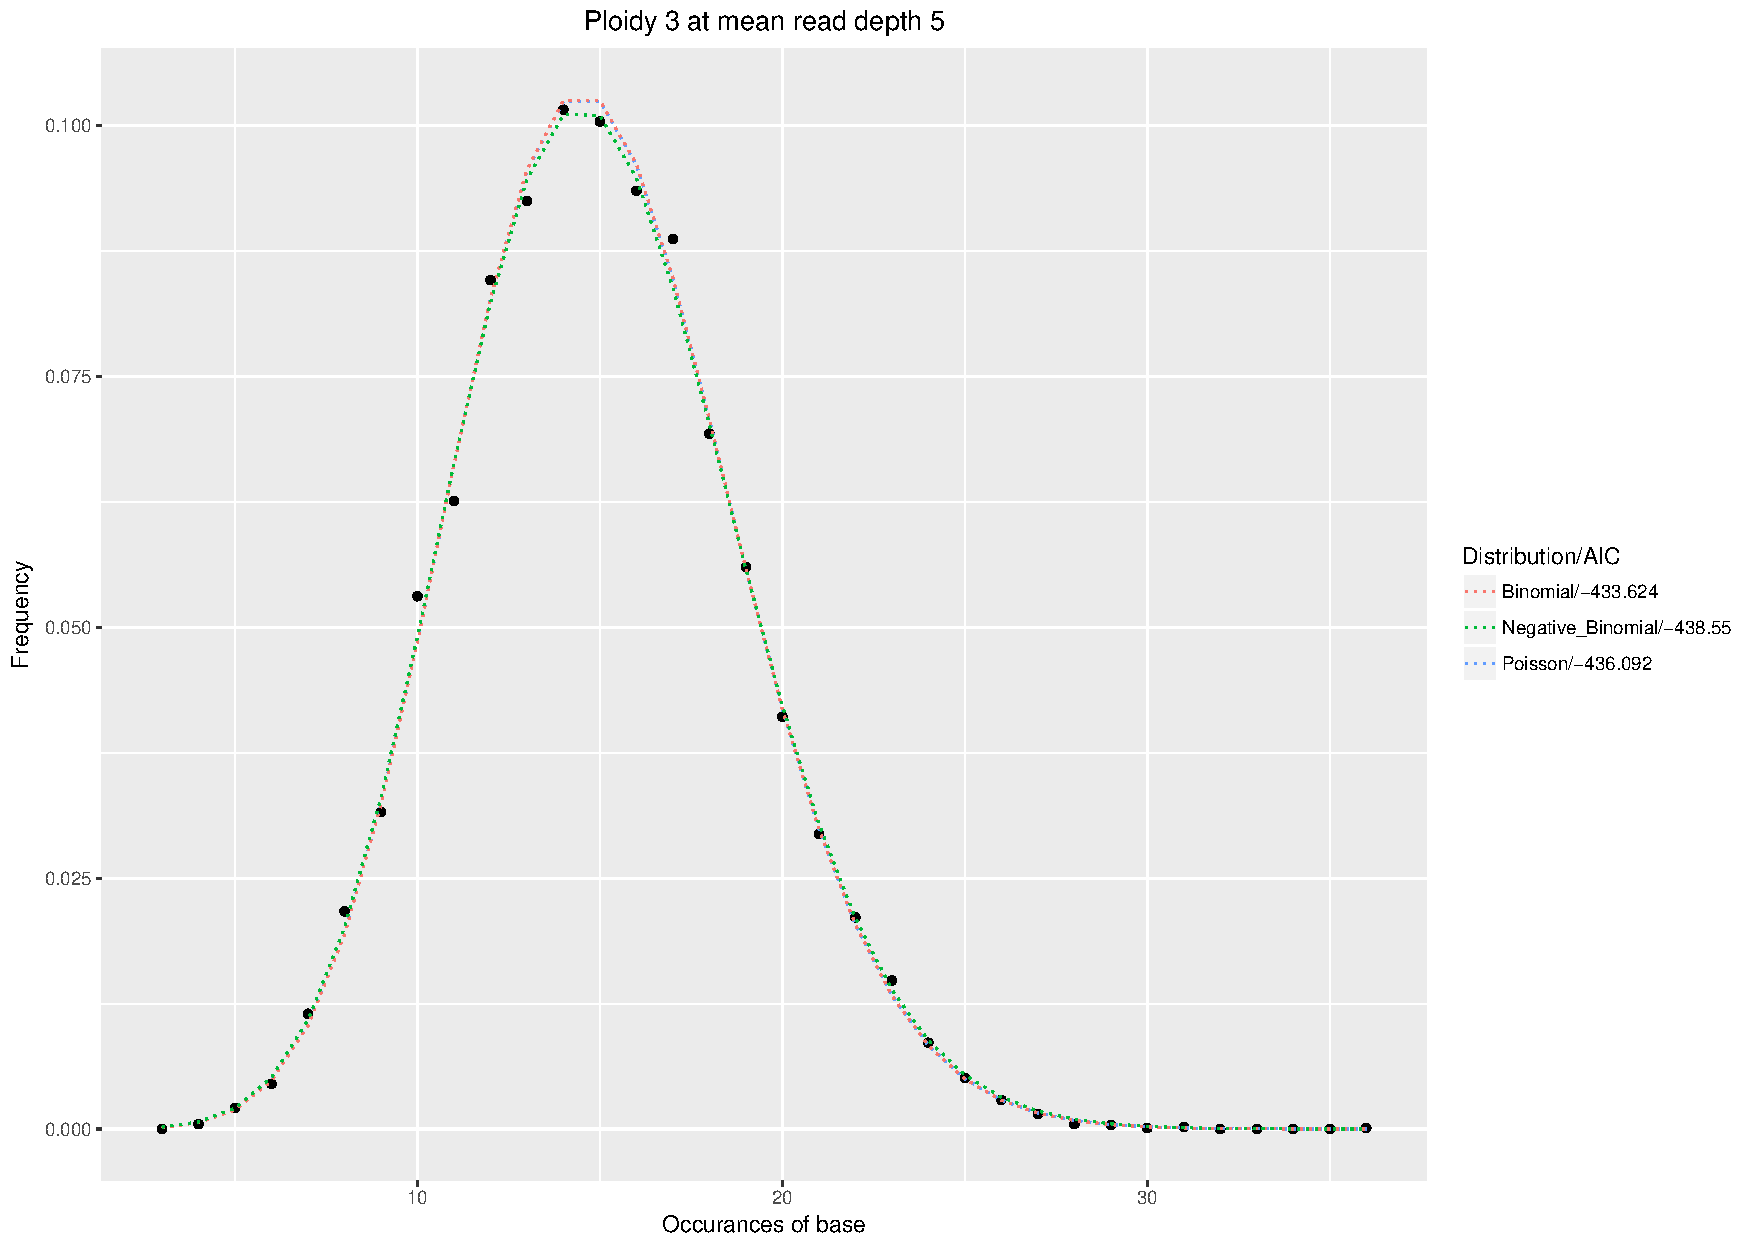
\includegraphics[scale=0.5]{../Results/Example_Fit_Constant_Ploidy.pdf}
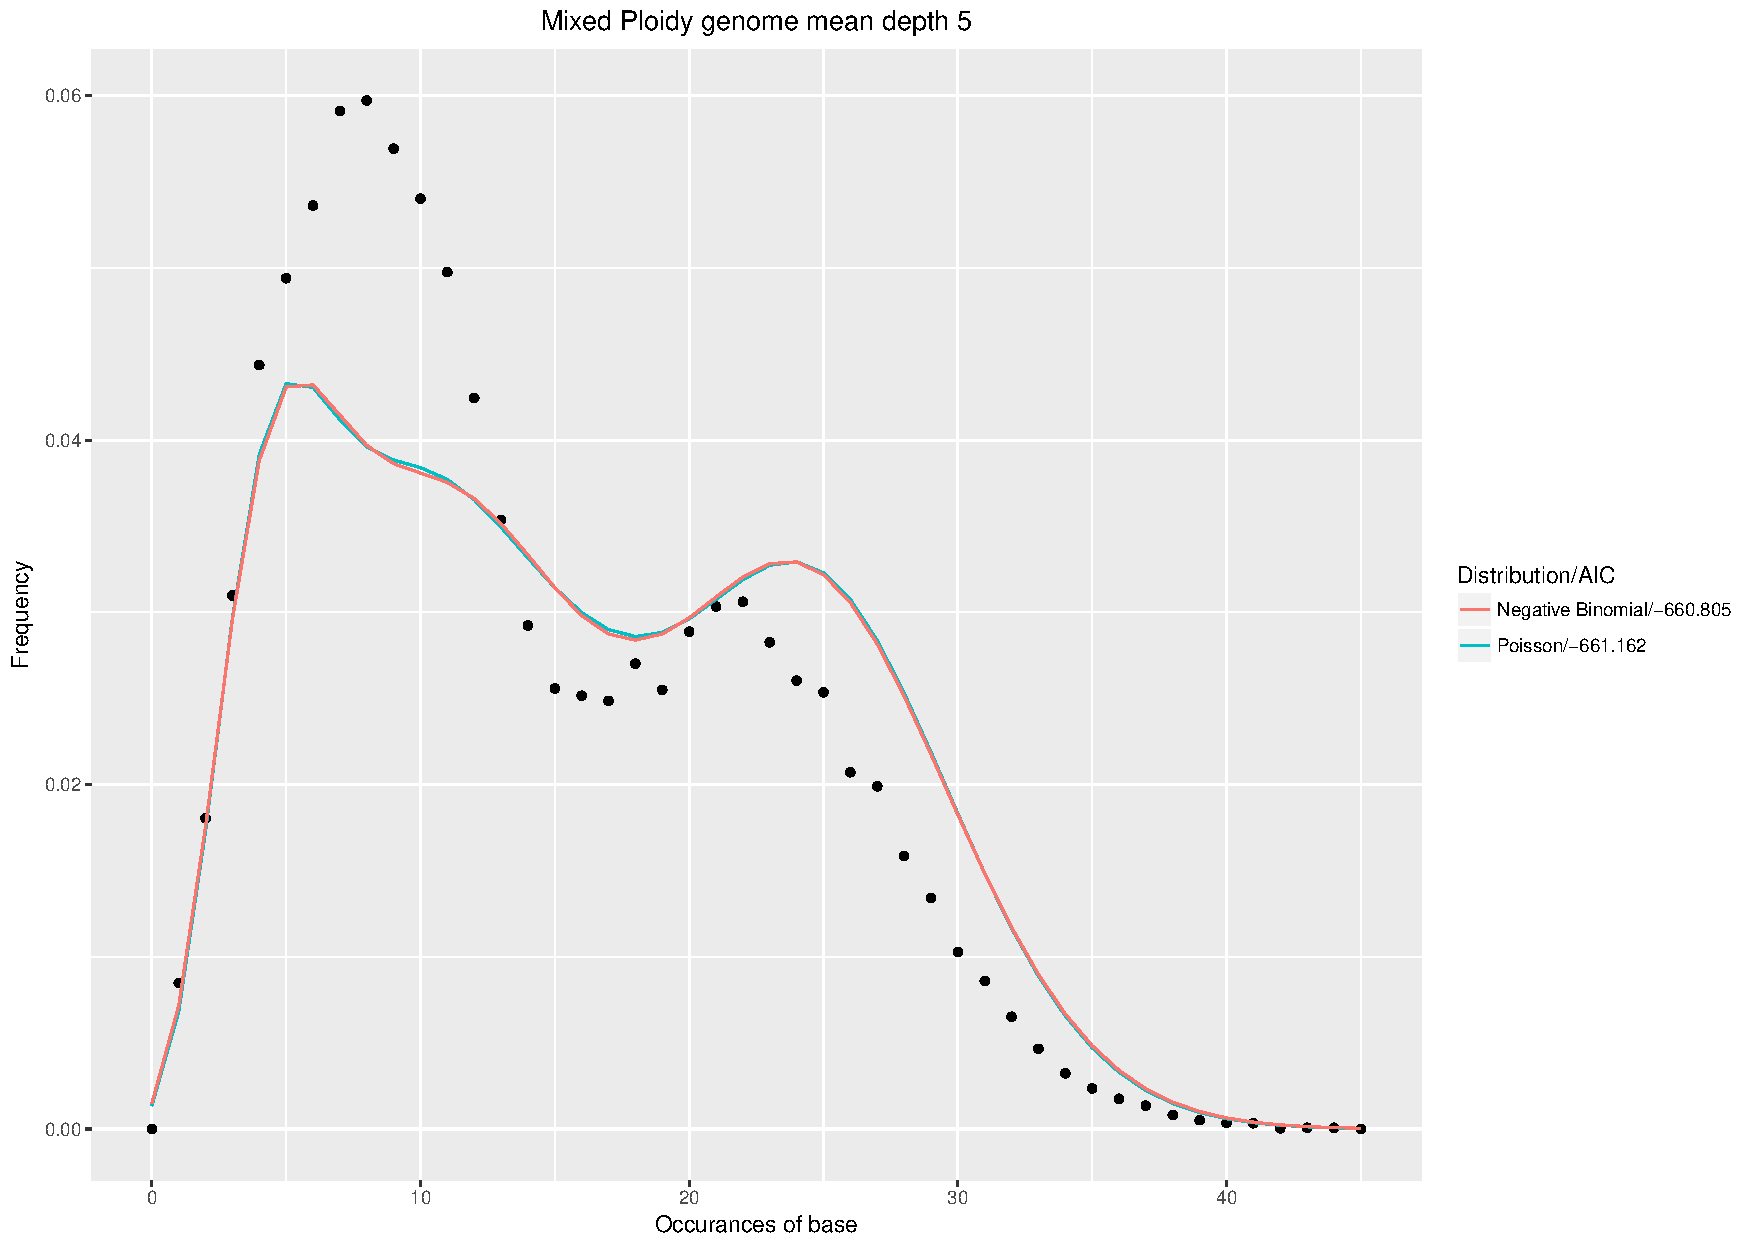
\includegraphics[scale=0.5]{../Results/Example_Fit_Mixed_Ploidy.pdf}
\caption{Visual examples of the resulting fitted distributions in both a constant and mixed ploidy state}
\end{center}

\end{figure}
%\begin{figure}[H]
%\begin{center}
%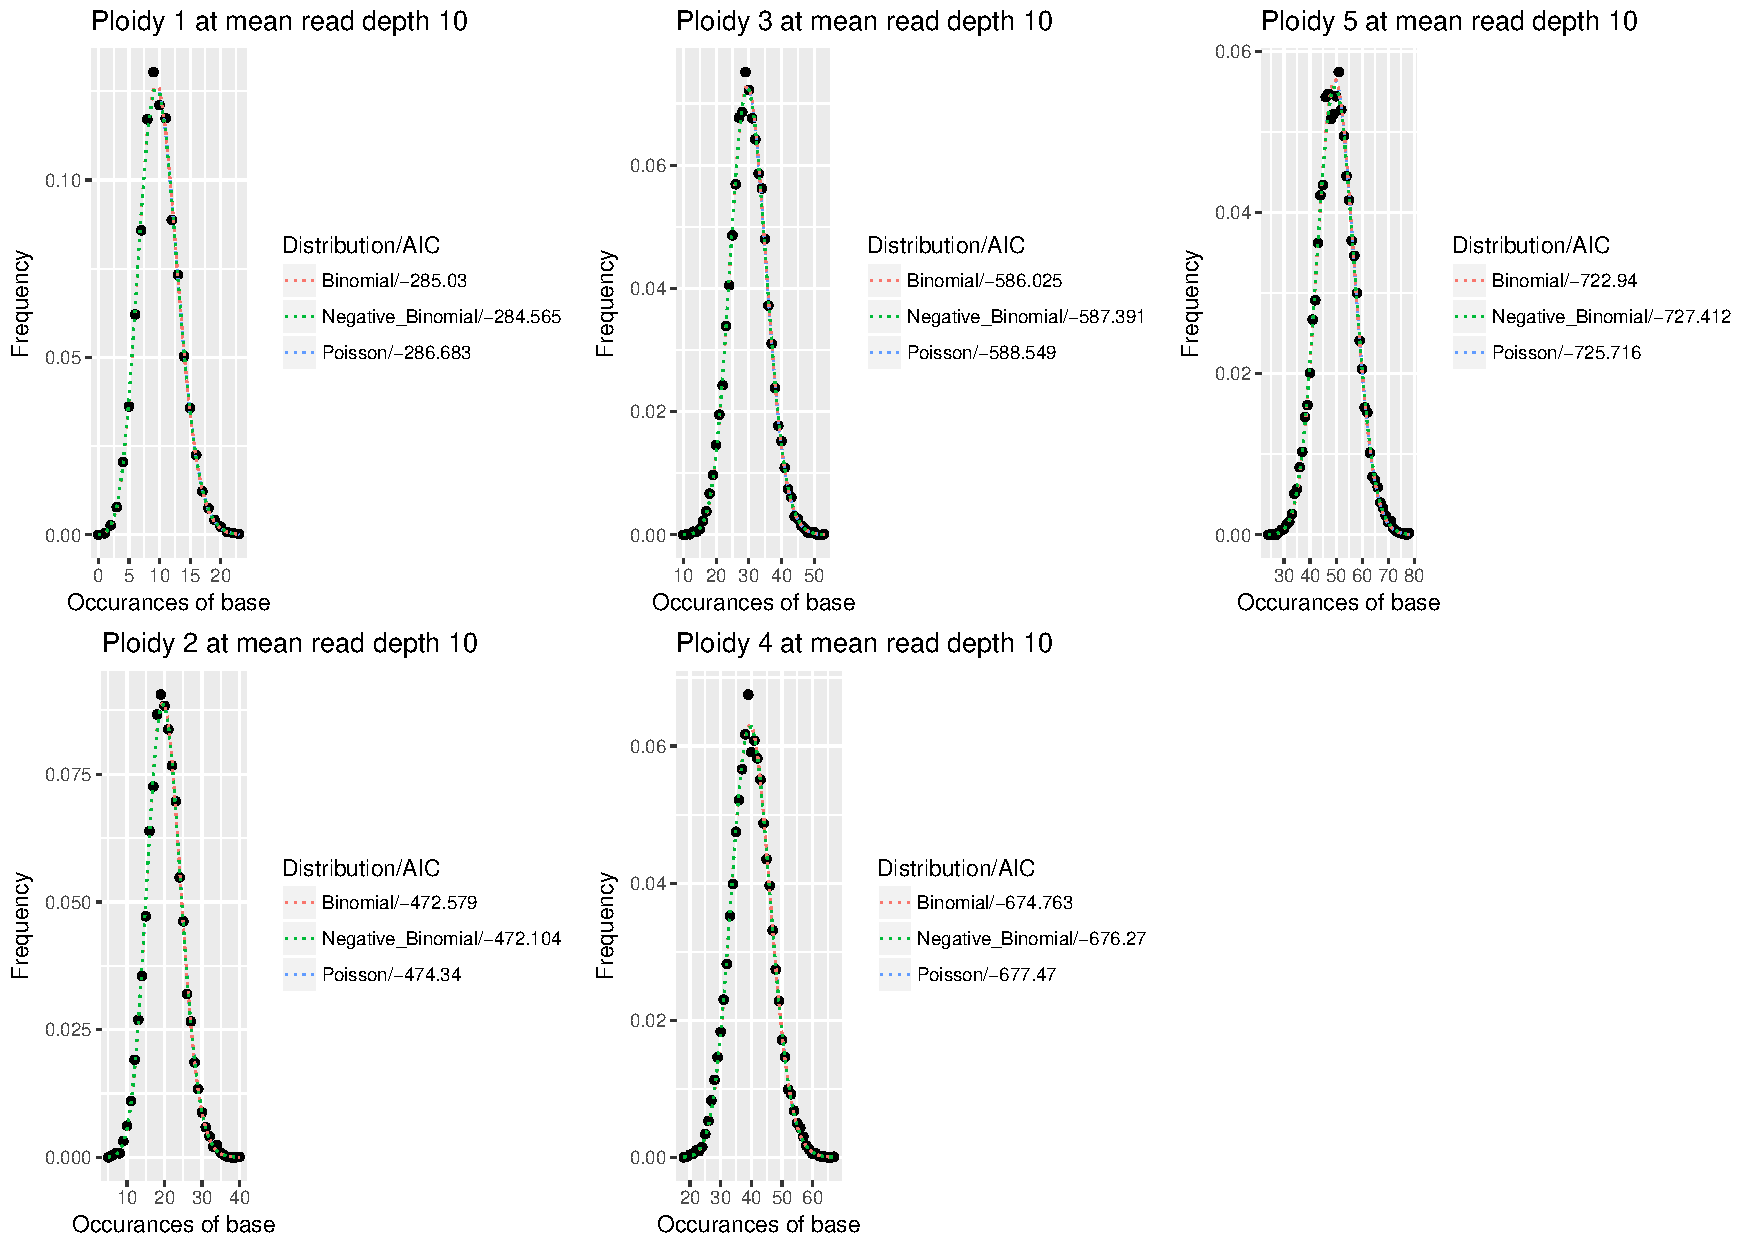
\includegraphics[scale=0.55]{../Results/First_Analysis/10/Fitted_Distributions_10.pdf}
%\caption{A visualisation of the fitted distributions at mean haploid depth 10 at constant ploidies 1-5}
%\end{center}
%\end{figure}

\begin{table}[H]
\begin{center}
\caption{AIC values for distributions fitted to genomes of uniform ploidy}
\begin{tabular}{|c|c|P{3.5cm}|P{3.5cm}|P{3.5cm}|}
\hline
\multirow{2}{*}{MHRD} & \multirow{2}{*}{Ploidy} & \multicolumn{3}{|c|}{Distributions} \\
\cline{3-5}
& & Poisson & Binomial & Negative Binomial \\
\hline
\multirow{5}{*}{2} & 1 & -53.685 & \underline{\textbf{-53.716}} & -51.680 \\
\cline{2-5}
& 2 & \underline{\textbf{-133.608}} & -131.579 & -133.041 \\
\cline{2-5}
& 3 & -199.852 & -197.619 & \underline{\textbf{-204.276}} \\
\cline{2-5}
& 4 & \underline{\textbf{-677.47}} & -674.763 & -676.27 \\
\cline{2-5}
& 5 & -266.329 & -263.786 & \underline{\textbf{-278.507}} \\
\hline
\multirow{5}{*}{5} & 1 & \underline{\textbf{-184.567}} & -182.505 & -182.973 \\
\cline{2-5}
& 2 & -287.548 & -285.311 &\underline{\textbf{-288.607}} \\
\cline{2-5}
& 3 & -436.092 & -433.624 & \underline{\textbf{-438.550}} \\
\cline{2-5}
& 4 & -418.225 & - 415.779 &  \underline{\textbf{-419.145}} \\
\cline{2-5}
& 5 & -495.524 & -492.785 & \underline{\textbf{-495.524}} \\
\hline
\multirow{5}{*}{10} & 1 & \underline{\textbf{-286.683}} & -285.03 & -284.565 \\
\cline{2-5}
& 2 & \underline{\textbf{-474.34}} & -472.579 & -472.104 \\
\cline{2-5}
& 3 & \underline{\textbf{-588.549}} & -586.025 & -587.391 \\
\cline{2-5}
& 4 & \underline{\textbf{-677.470}} & -674.763 & -676.270 \\
\cline{2-5}
& 5 & -725.716 & -722.940 & \underline{\textbf{-727.412}} \\
\hline
\multirow{5}{*}{25} & 1 & -551.252 & -548.725 & \underline{\textbf{-551.901}} \\
\cline{2-5}
& 2 & -811.257 & -811.267 & \underline{\textbf{-820.839}} \\
\cline{2-5}
& 3 & -945.114 & -942.279 & \underline{\textbf{-952.674}} \\
\cline{2-5}
& 4 & -1022.209 & -1018.891 & \underline{\textbf{-1039.926}} \\
\cline{2-5}
& 5 & -1256.798 & -1252.42 & \underline{\textbf{-1284.00}} \\
\hline
\multirow{5}{*}{50} & 1 & -789.793 & -786.414 & \underline{\textbf{-805.149}} \\
\cline{2-5}
& 2 & -1046.17 & -1042.534 & \underline{\textbf{-1060.249}} \\
\cline{2-5}
& 3 & -1354.387 & -1349.491 & \underline{\textbf{-1426.747}} \\
\cline{2-5}
& 4 & -1528.782 & -1523.729 & \underline{\textbf{-1530.324}} \\
\cline{2-5}
& 5 & -1758.35 & -1753.272 & \underline{\textbf{-1760.201}} \\
\hline


\end{tabular}
\end{center}
\caption*{MHRD: Mean haploid read depth, i.e the average read depth of part of the genome that would be found in haploid state}
\end{table}
For speed and efficiency in simulation the Binomial distribution was omitted for the study of mixed ploidy cases due to its performance for the cases where the genomes had a constant ploidy. During the mixed ploidy cases, when the genome was structured with a ploidy increasing step-wise for each chromosome, the mixture of Poisson distributions performed better at lower mean haploid read depths (10 and below) but the the Negative binomial was better at higher depths (greater than 50) whilst at 25 it was a fairly even split between the two distributions (Figure 2). The difference between the distributions became more notable as the number of different ploidies within the genome increased.

\begin{figure}
\begin{center}
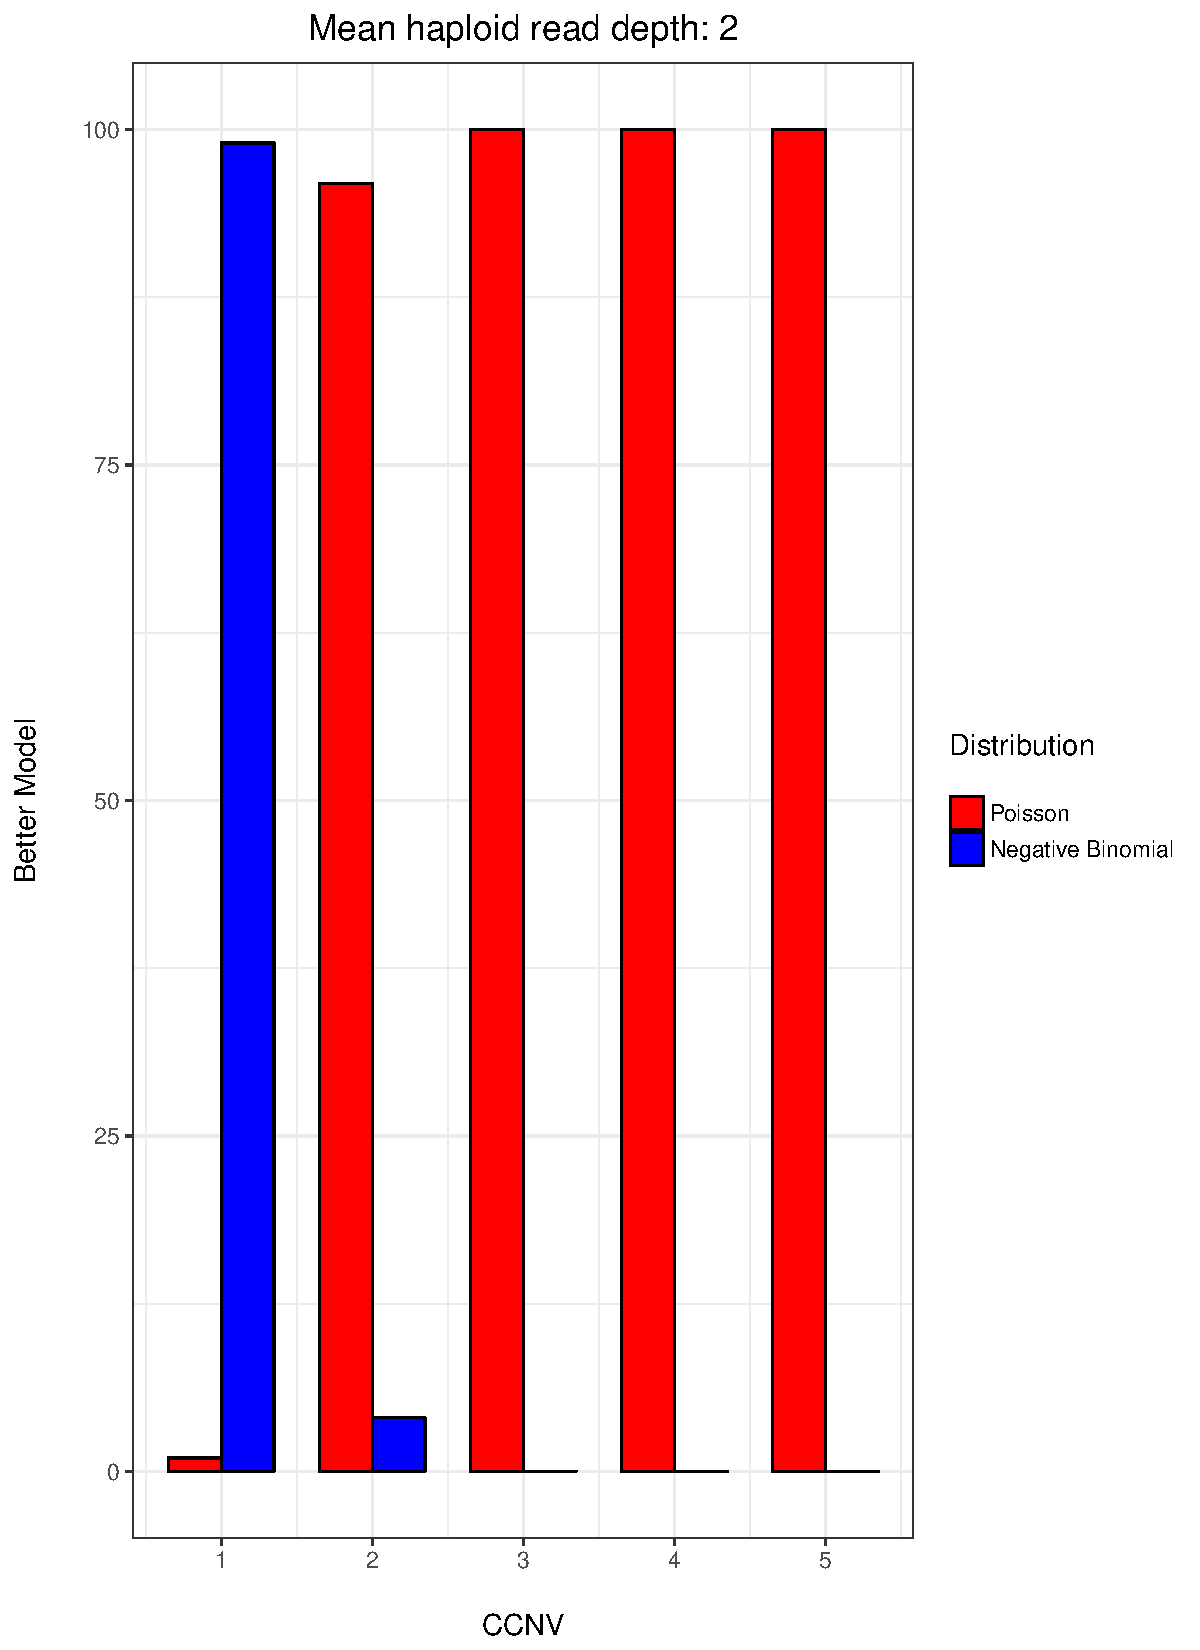
\includegraphics[scale=0.28]{../Results/Second_Analysis/Better_model_bar2.pdf}
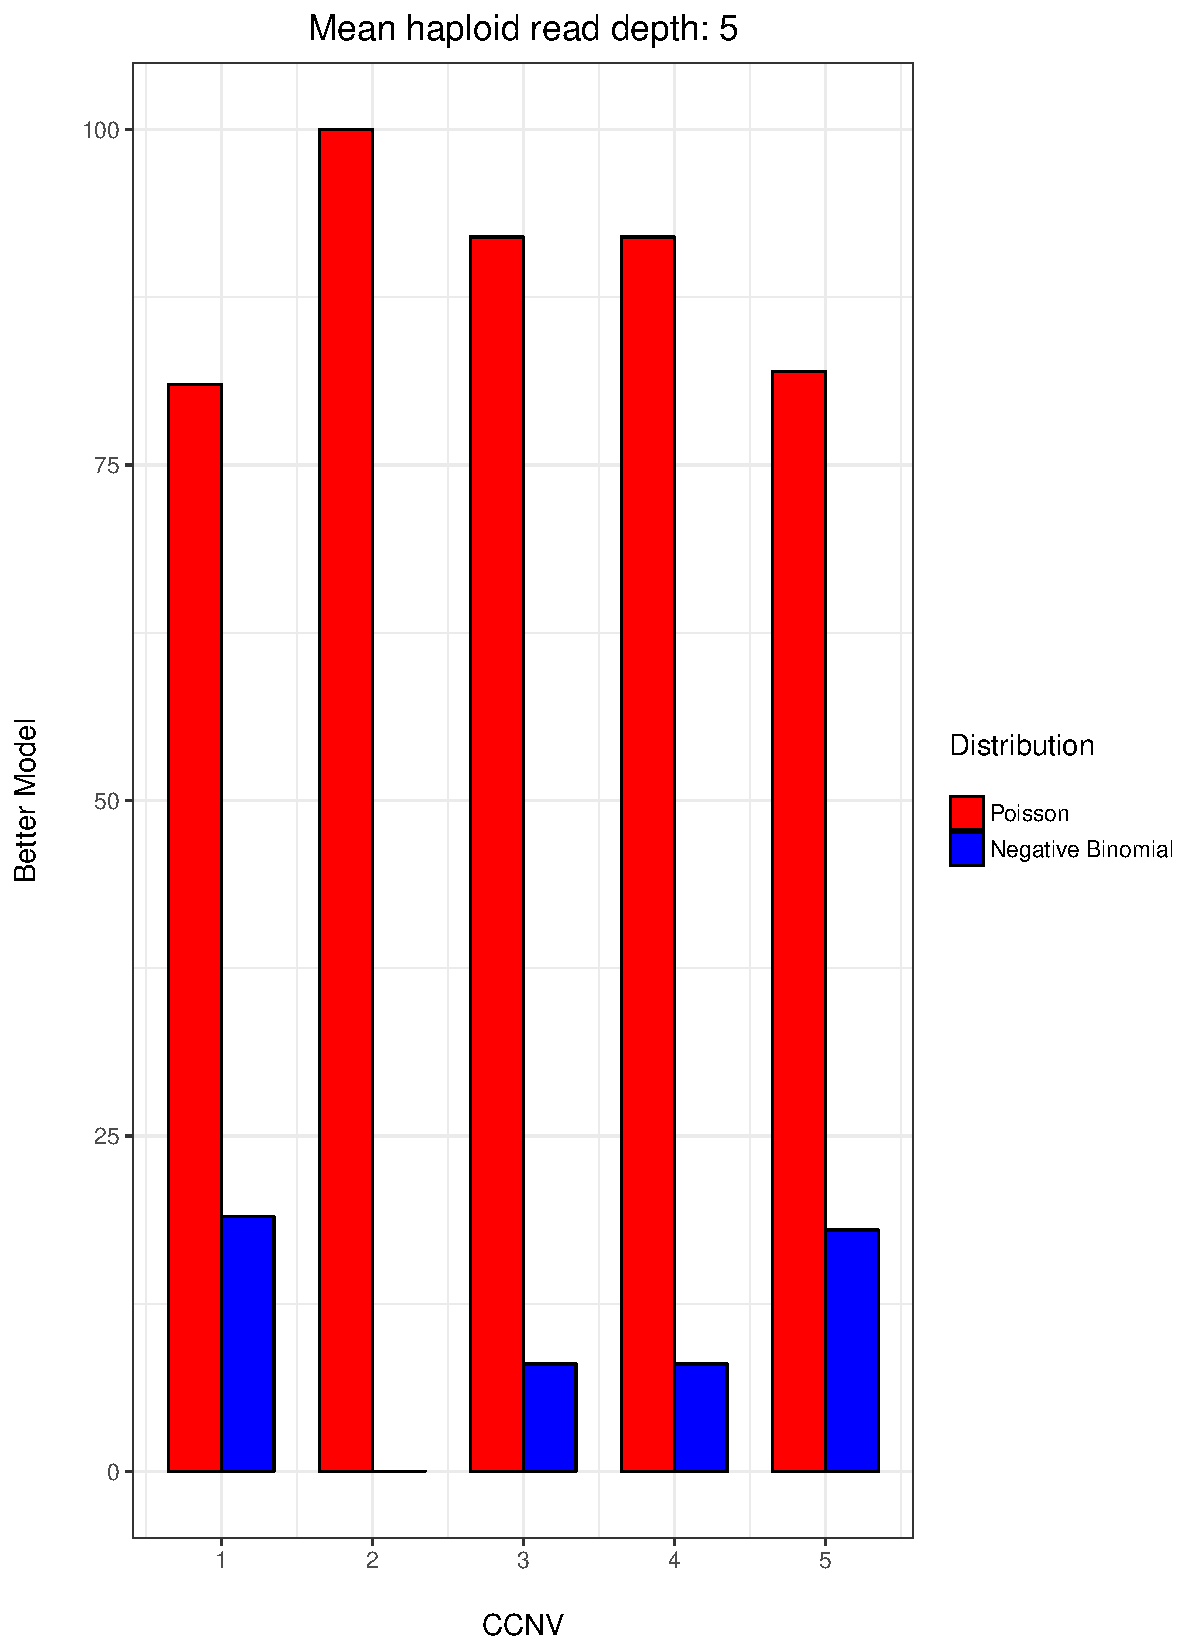
\includegraphics[scale=0.28]{../Results/Second_Analysis/Better_model_bar5.pdf}
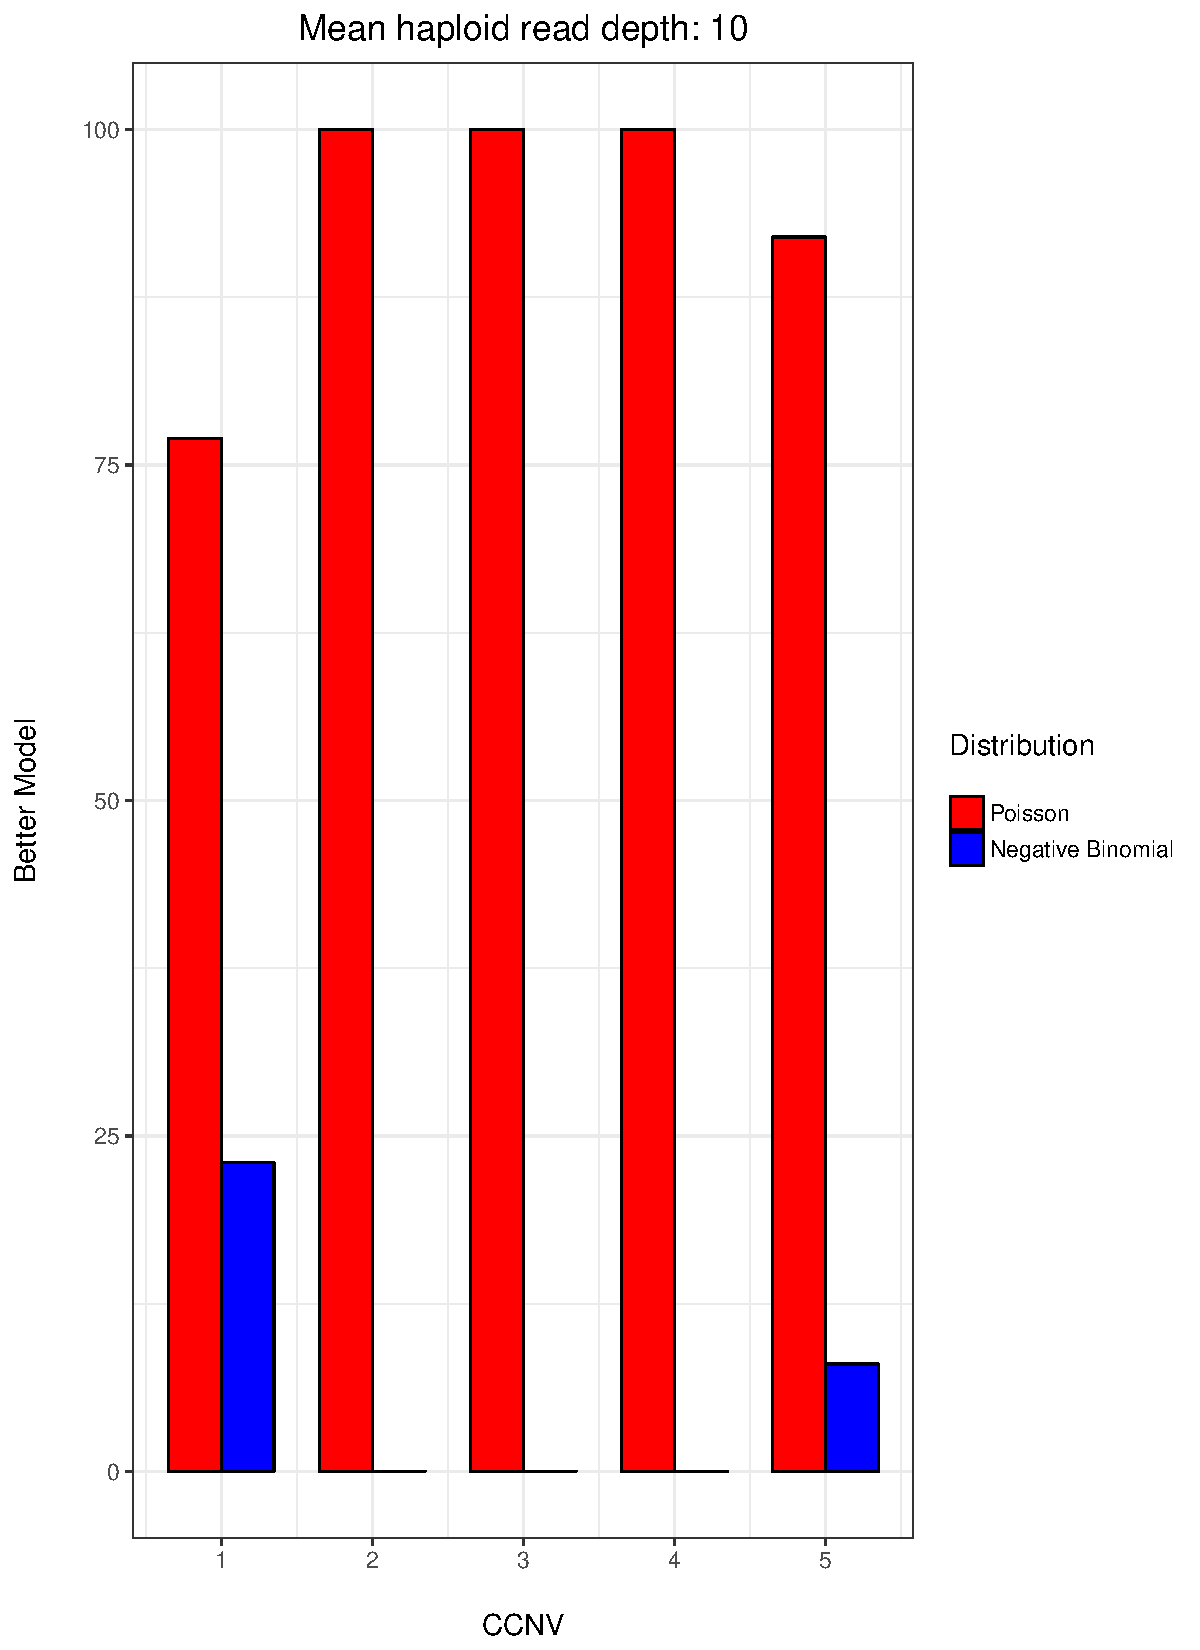
\includegraphics[scale=0.28]{../Results/Second_Analysis/Better_model_bar10.pdf}
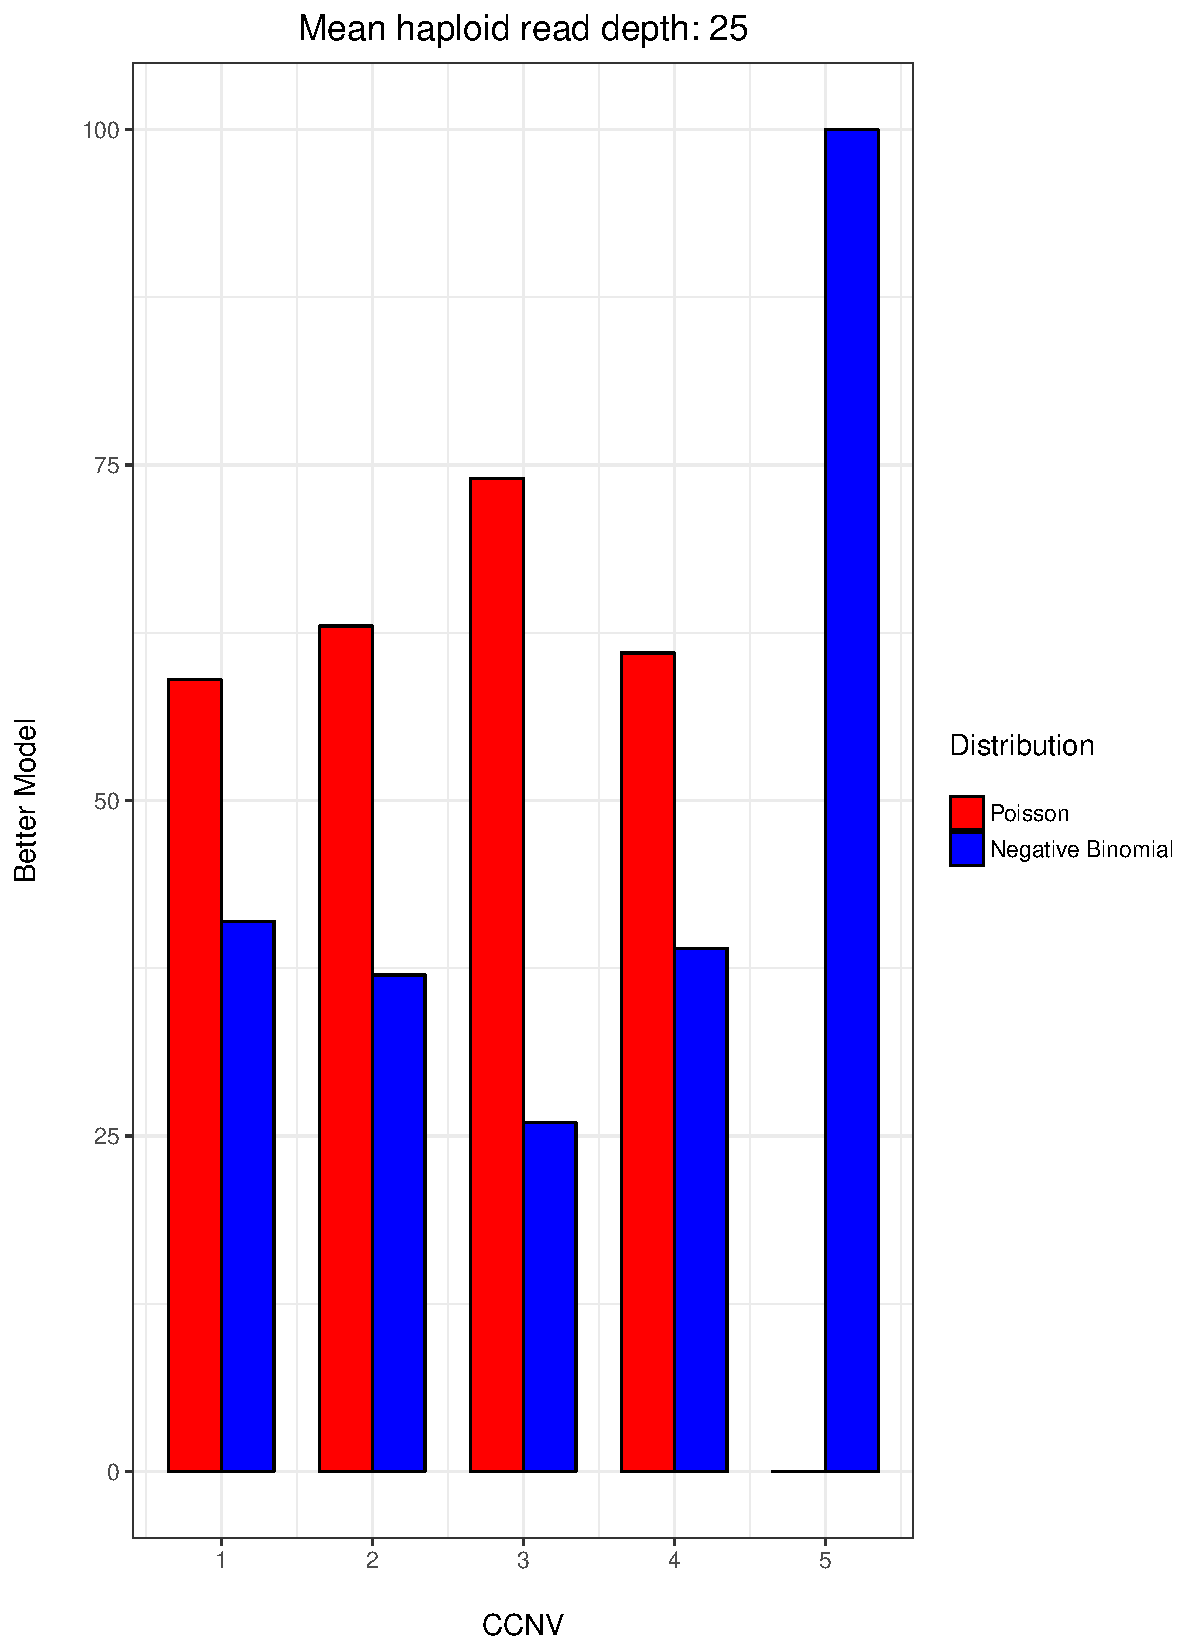
\includegraphics[scale=0.28]{../Results/Second_Analysis/Better_model_bar25.pdf}
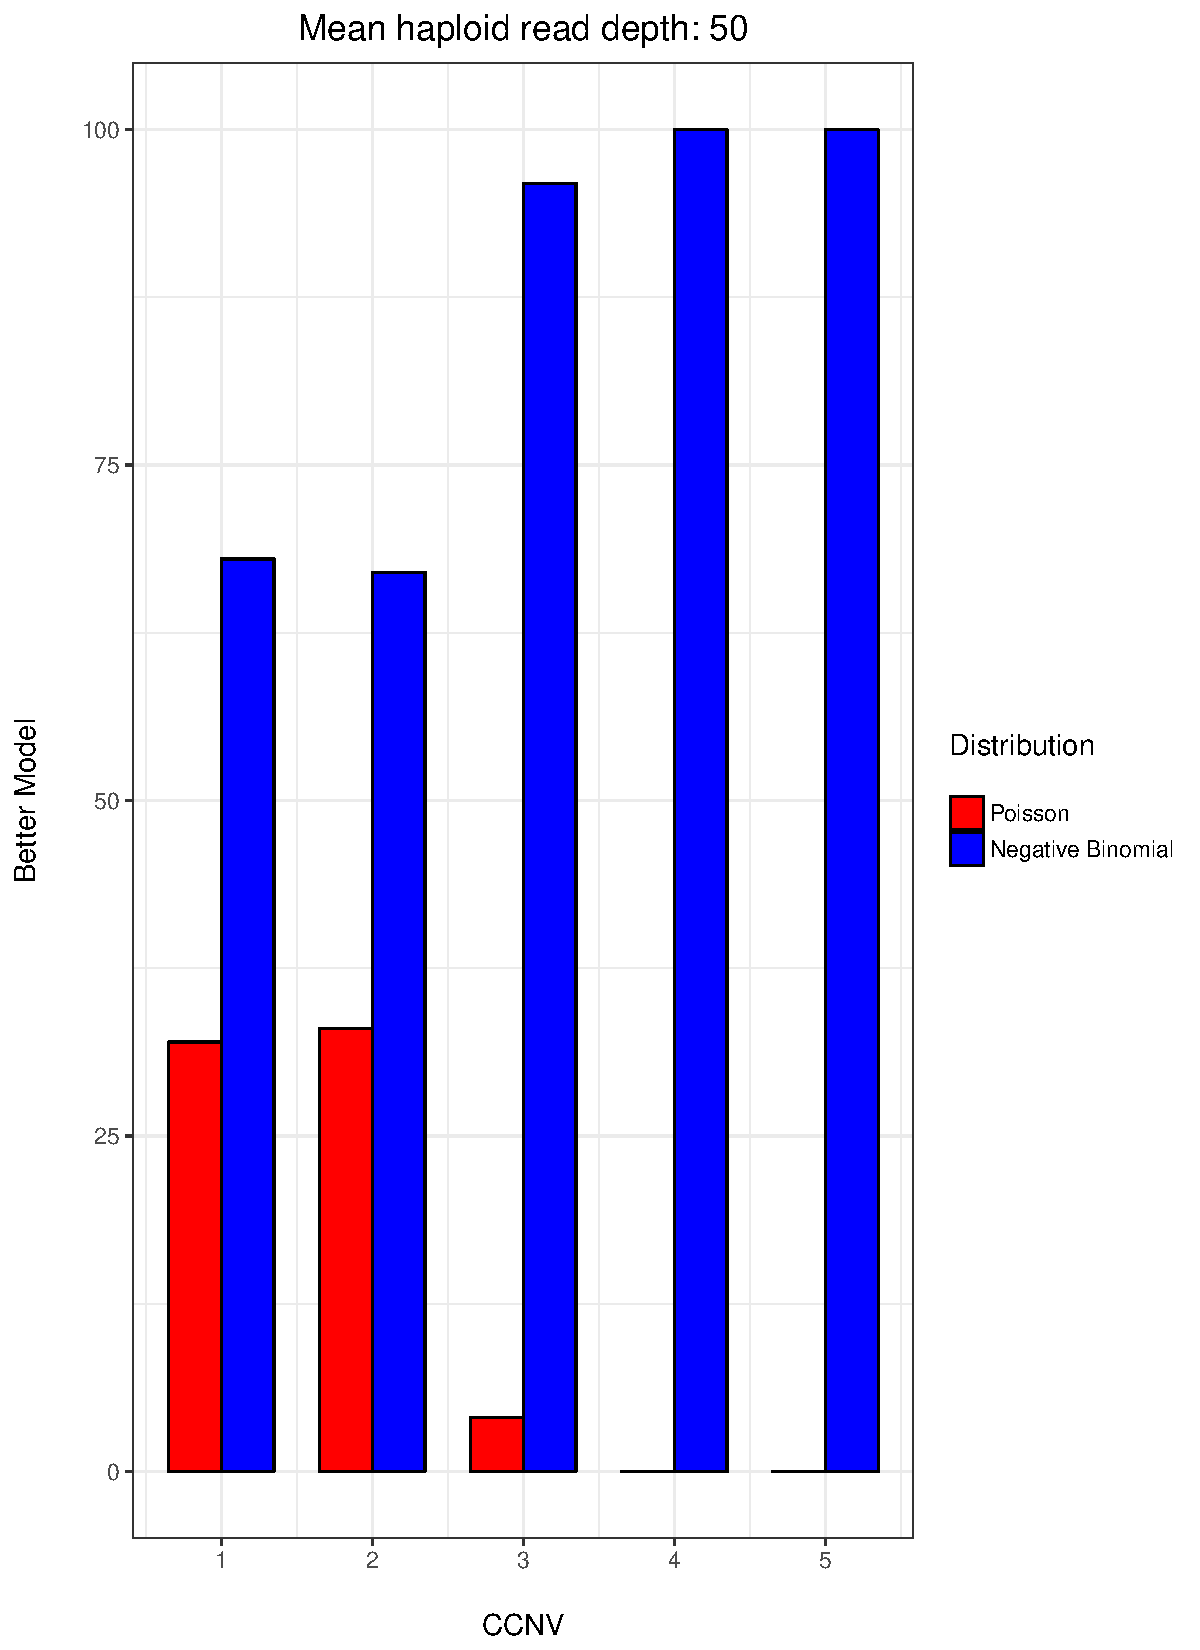
\includegraphics[scale=0.28]{../Results/Second_Analysis/Better_model_bar50.pdf}
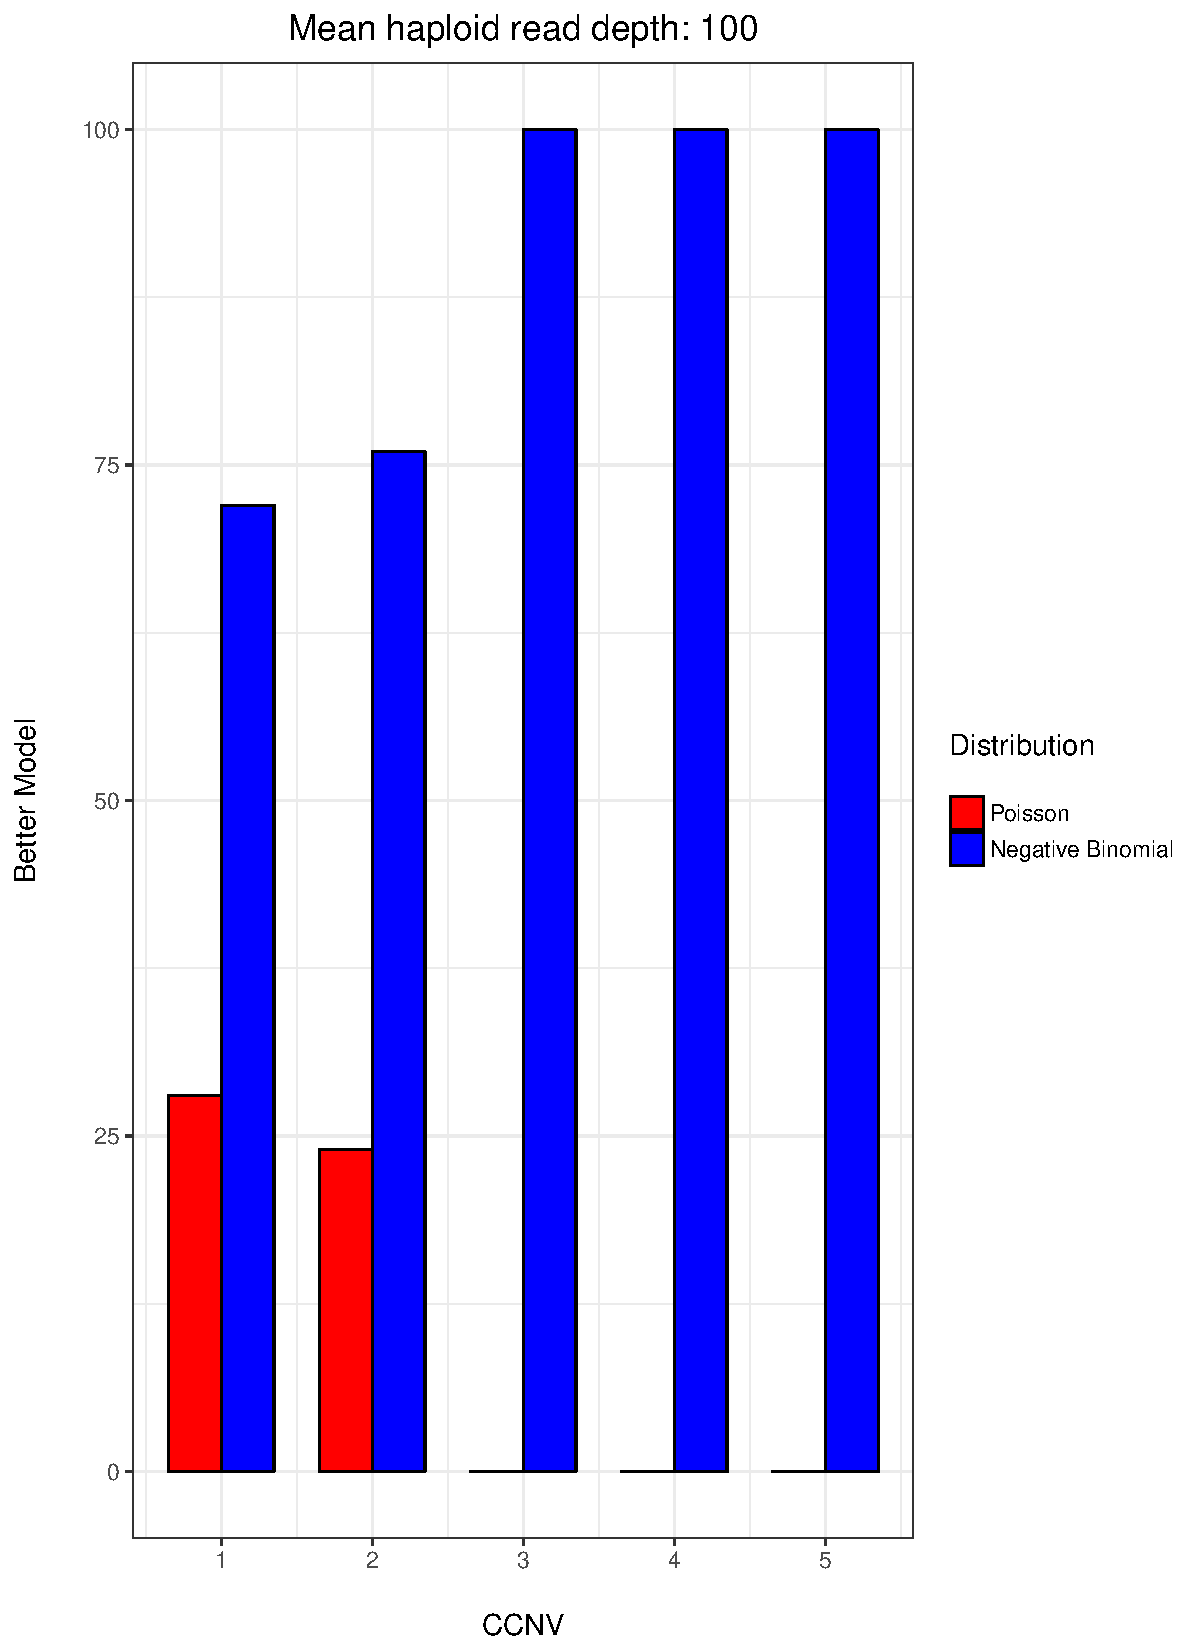
\includegraphics[scale=0.28]{../Results/Second_Analysis/Better_model_bar100.pdf}
\end{center}
\caption{Bar plots comparing the number of occurances when each distribution's mixture model fitted better at each mean haploid read depth}
\end{figure}


%\begin{table}[H]
%\begin{center}
%\caption{Number of occurrences when each mixture distribution had the lower AIC value}
%\begin{tabular}{|c|c||P{4cm}|P{4cm}|}
%\hline
%\multirow{2}{*}{\textbf{MHRD}} & \multirow{2}{*}{\textbf{CCNV}} & \multicolumn{2}{|c|}{\textbf{Distributions mixture}} \\
%\cline{3-4}
%& & \textbf{Poisson} & \textbf{Negative Binomial} \\
%\hline
%\hline
%\multirow{6}{*}{\textbf{10}} & 1 & 77  & 23 \\
%\cline{2-4}
%& 2 & 100 & 0 \\
%\cline{2-4}
%& 3 & 100 & 0 \\
%\cline{2-4}
%& 4 & 100 & 0 \\
%\cline{2-4}
%& 5 & 92 & 8 \\
%\cline{2-4}
%& \textbf{Total} & 469 & 31 \\
%\hline
%\hline
%\multirow{6}{*}{\textbf{25}} & 1 & 59  & 41 \\
%\cline{2-4}
%& 2 & 63 & 37 \\
%\cline{2-4}
%& 3 & 74 & 26 \\
%\cline{2-4}
%& 4 & 61 & 39 \\
%\cline{2-4}
%& 5 & 0 & 100 \\
%\cline{2-4}
%& \textbf{Total} & 257 & 243 \\
%\hline
%\hline
%\multirow{6}{*}{\textbf{50}} & 1 & 32 & 68 \\
%\cline{2-4}
%& 2 & 33 & 67 \\
%\cline{2-4}
%& 3 & 4 & 96 \\
%\cline{2-4}
%& 4 & 0 & 100 \\
%\cline{2-4}
%& 5 & 0 & 100 \\
%\cline{2-4}
%& \textbf{Total} & 69 & 431 \\
%\hline
%\hline
%\multirow{6}{*}{\textbf{100}} & 1 & 28  & 72 \\
%\cline{2-4}
%& 2 & 24 & 76 \\
%\cline{2-4}
%& 3 & 0 & 100 \\
%\cline{2-4}
%& 4 & 0 & 100 \\
%\cline{2-4}
%& 5 & 0 & 100 \\
%\cline{2-4}
%& \textbf{Total} & 52 & 448 \\
%\hline
%\hline
%\multicolumn{2}{|c||}{\textbf{Overall Totals}} & 847 & 1153 \\
%\hline
%\end{tabular}
%\caption*{MHRD: Mean haploid read depth, i.e the average read depth of part of the genome that would be found in haploid state\\
%CCNV: Chromosome copy number variation, representing the number of different ploidy levels in each genome}
%\end{center}
%\end{table}
Comparing the number of distributions in the optimal mixture model to the actual ploidy variation of the genome, the Poisson mixture distribution performs better at predicting the amount of ploidy variation in the genome at very low mean haploid read depths. However, the Negative binomial mixture distributions perform better at higher mean haploid read depths where the Poisson distribution seem to have a tendency to be over-fitted to the genome. This pattern has a clear correlation with the mean haploid read depths and is reflected both in the confusion matrices  and the corresponding root mean standard deviation (RMSD) values (Figure 3-4, Table 2). 
\begin{figure}[H]
\begin{center}
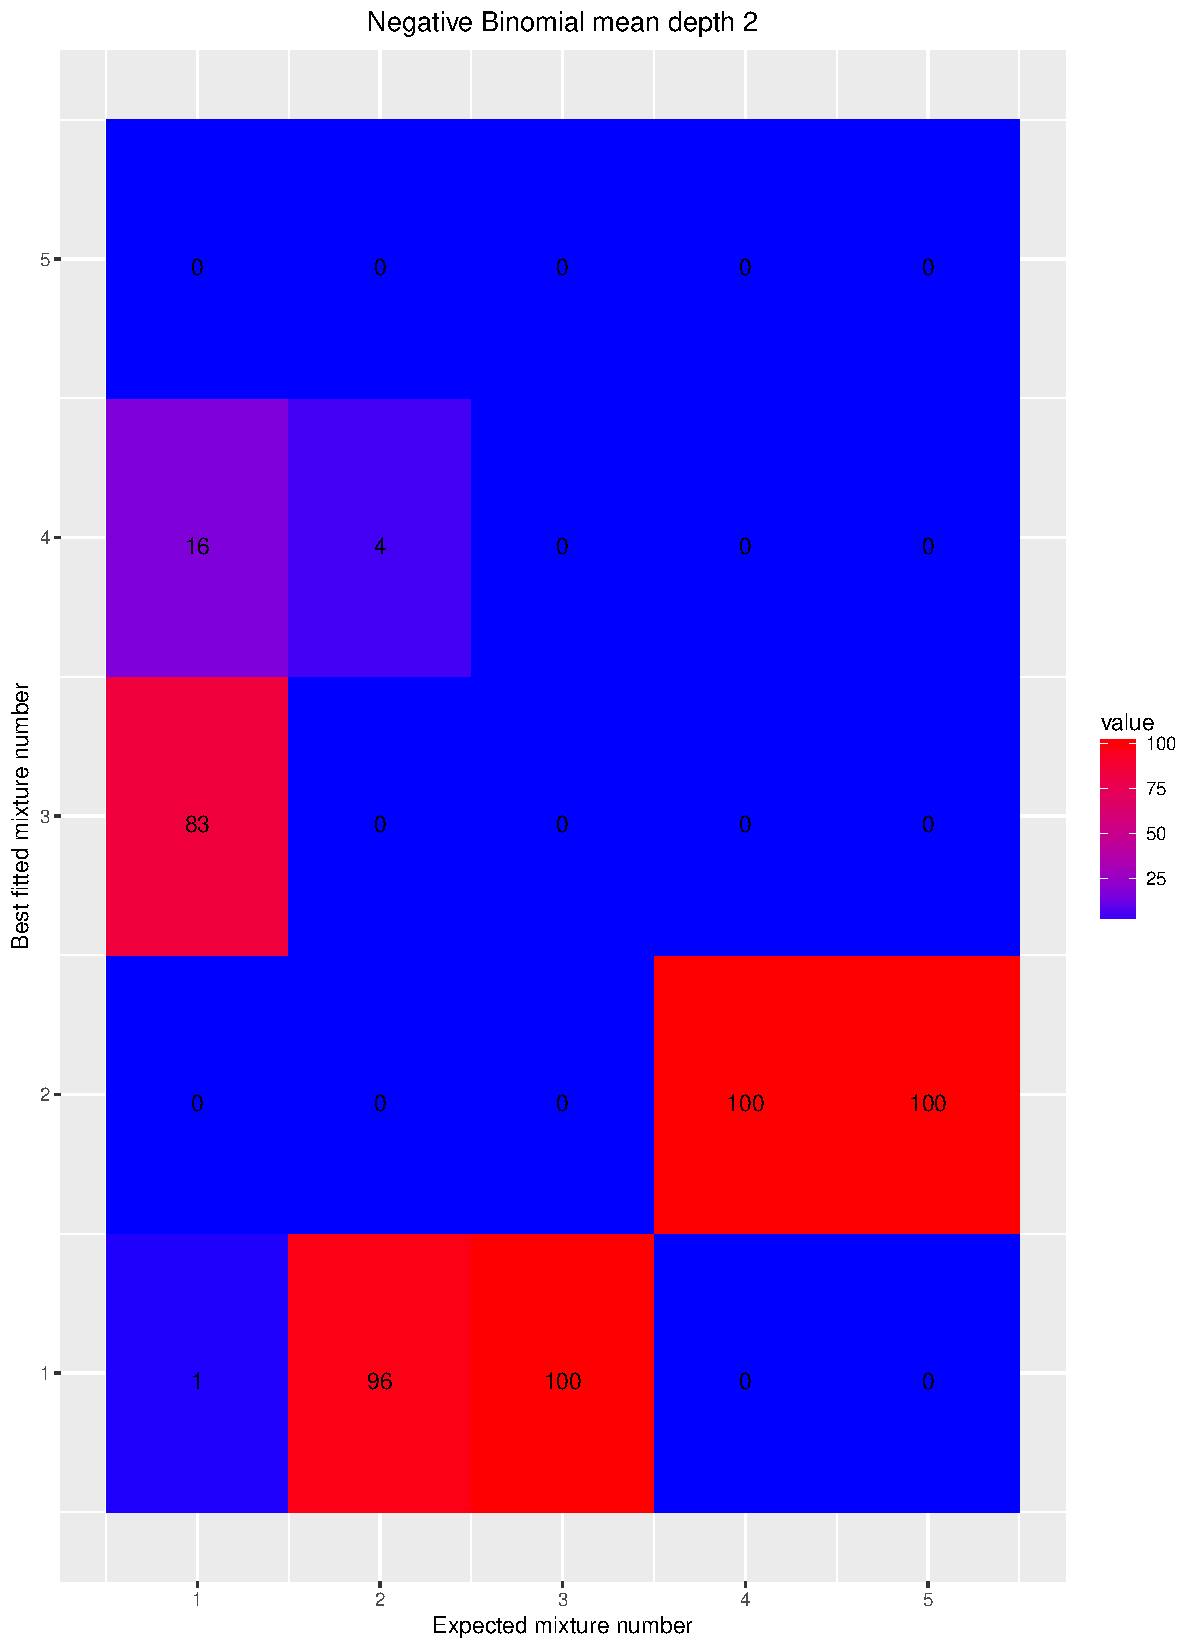
\includegraphics[scale=0.27]{../Results/Second_Analysis/Negative_Binomial_Confusion_Matrix_2.pdf}
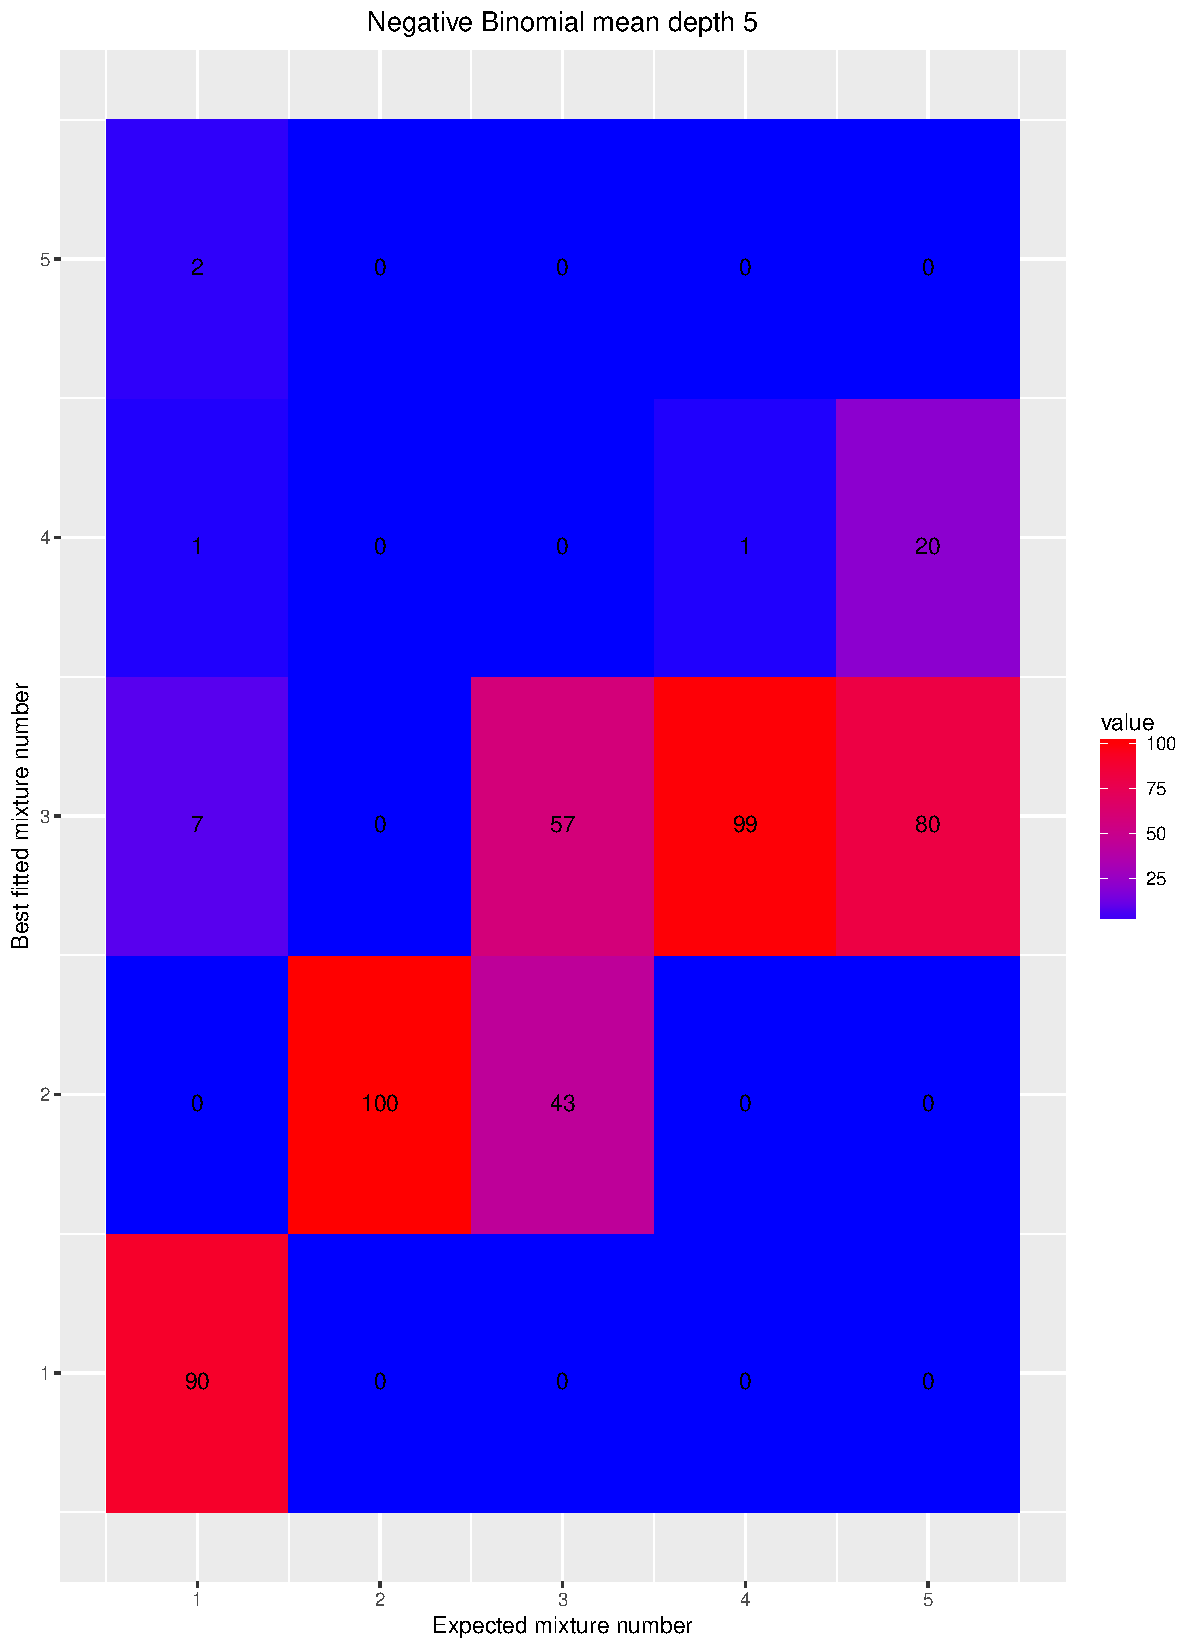
\includegraphics[scale=0.27]{../Results/Second_Analysis/Negative_Binomial_Confusion_Matrix_5.pdf}
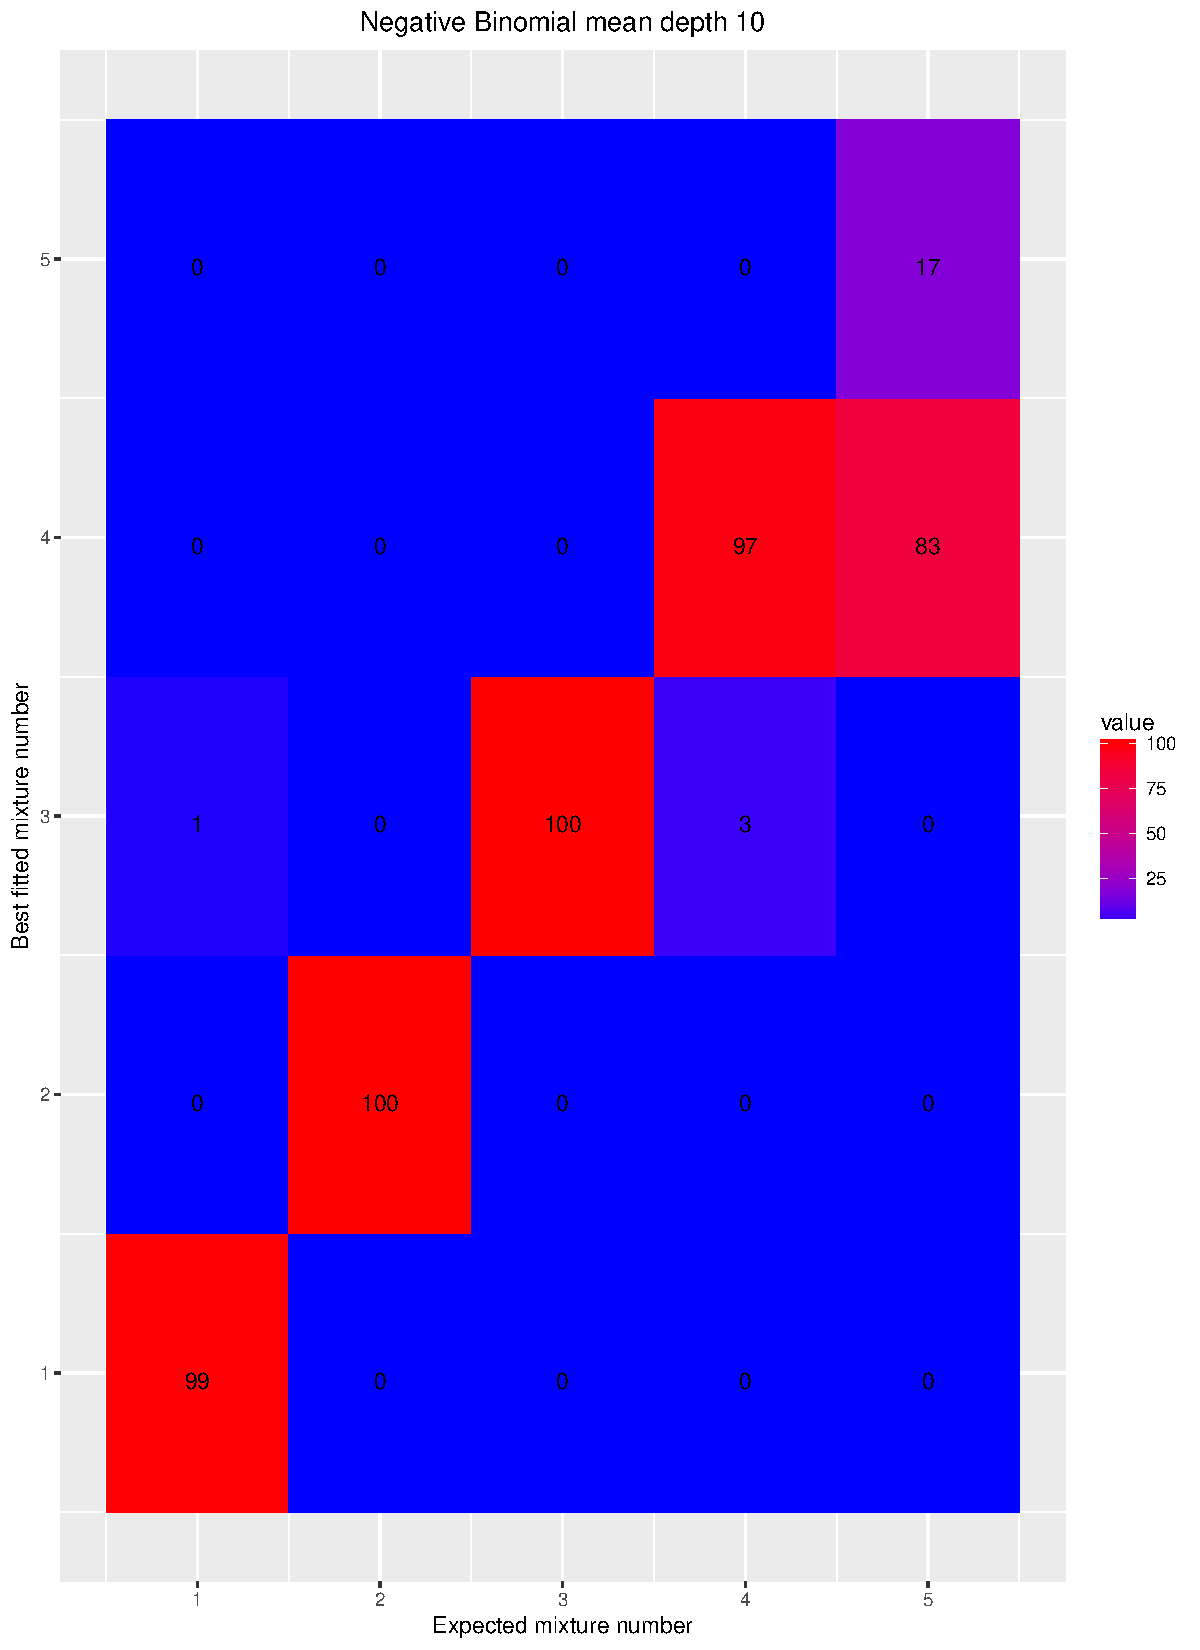
\includegraphics[scale=0.27]{../Results/Second_Analysis/Negative_Binomial_Confusion_Matrix_10.pdf}
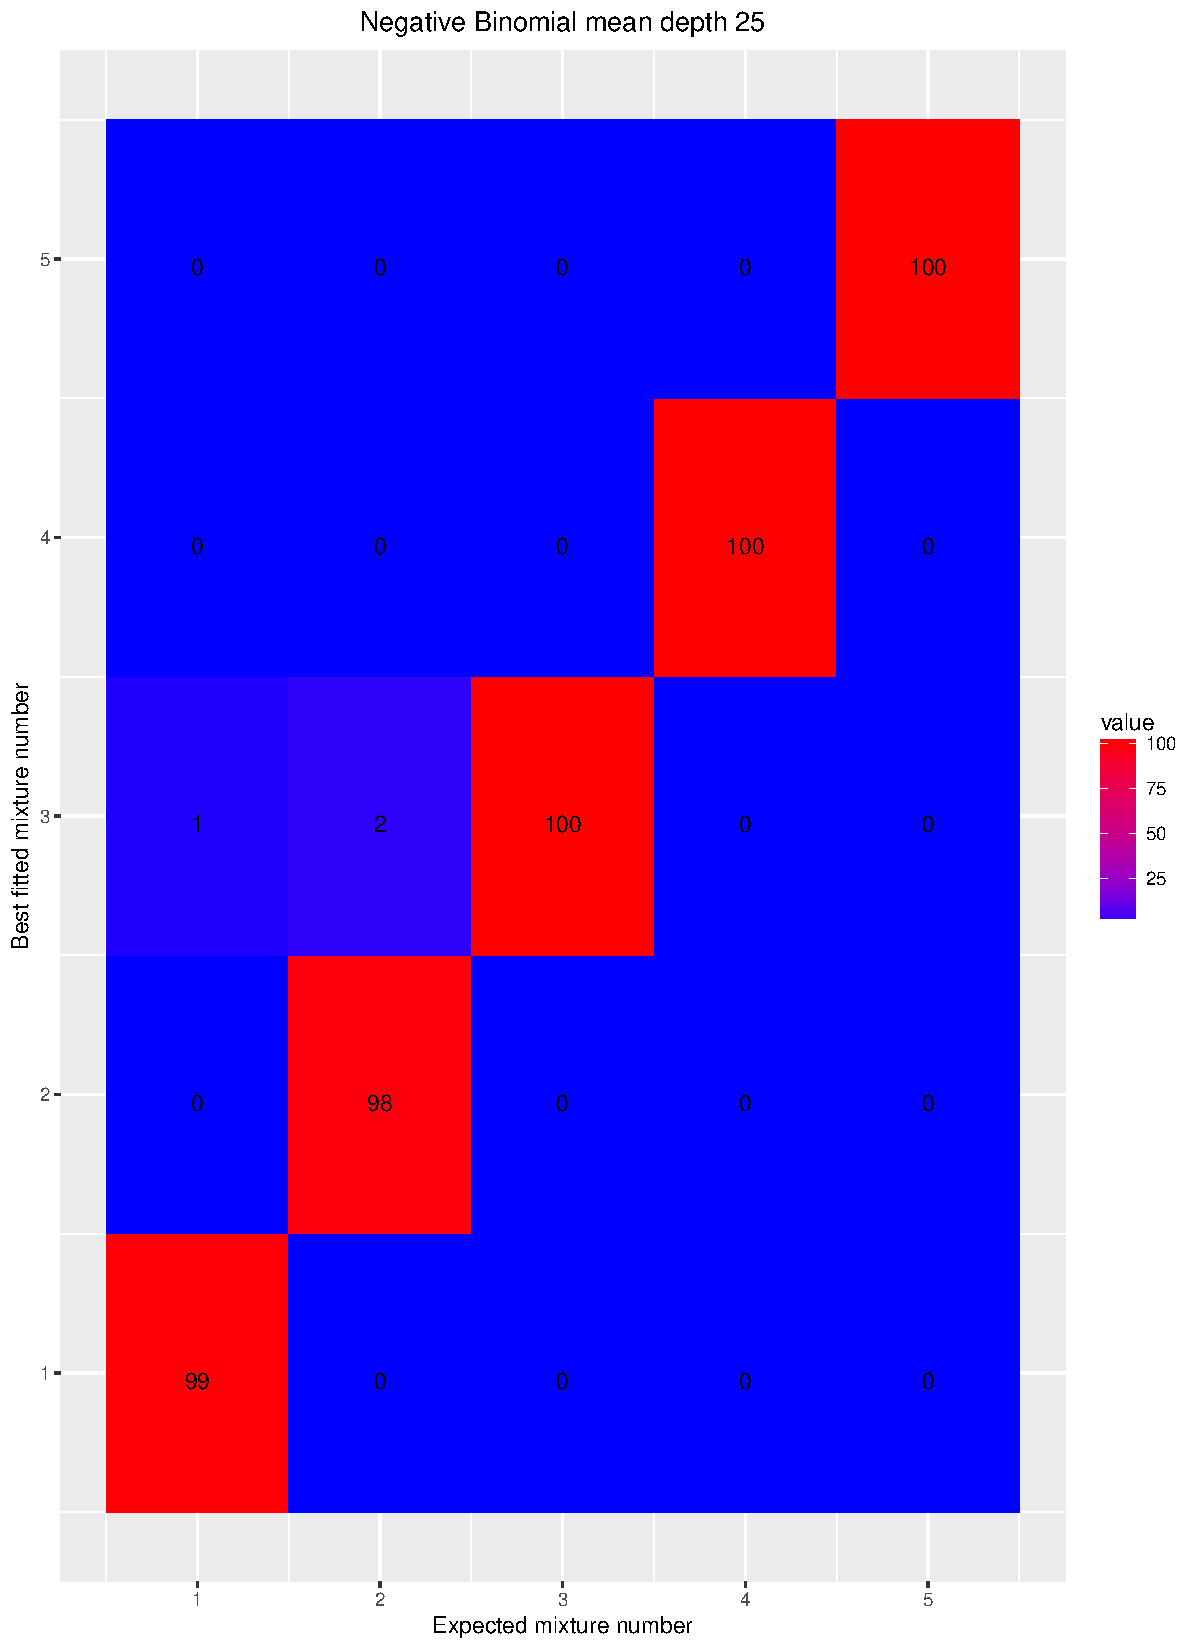
\includegraphics[scale=0.27]{../Results/Second_Analysis/Negative_Binomial_Confusion_Matrix_25.pdf}
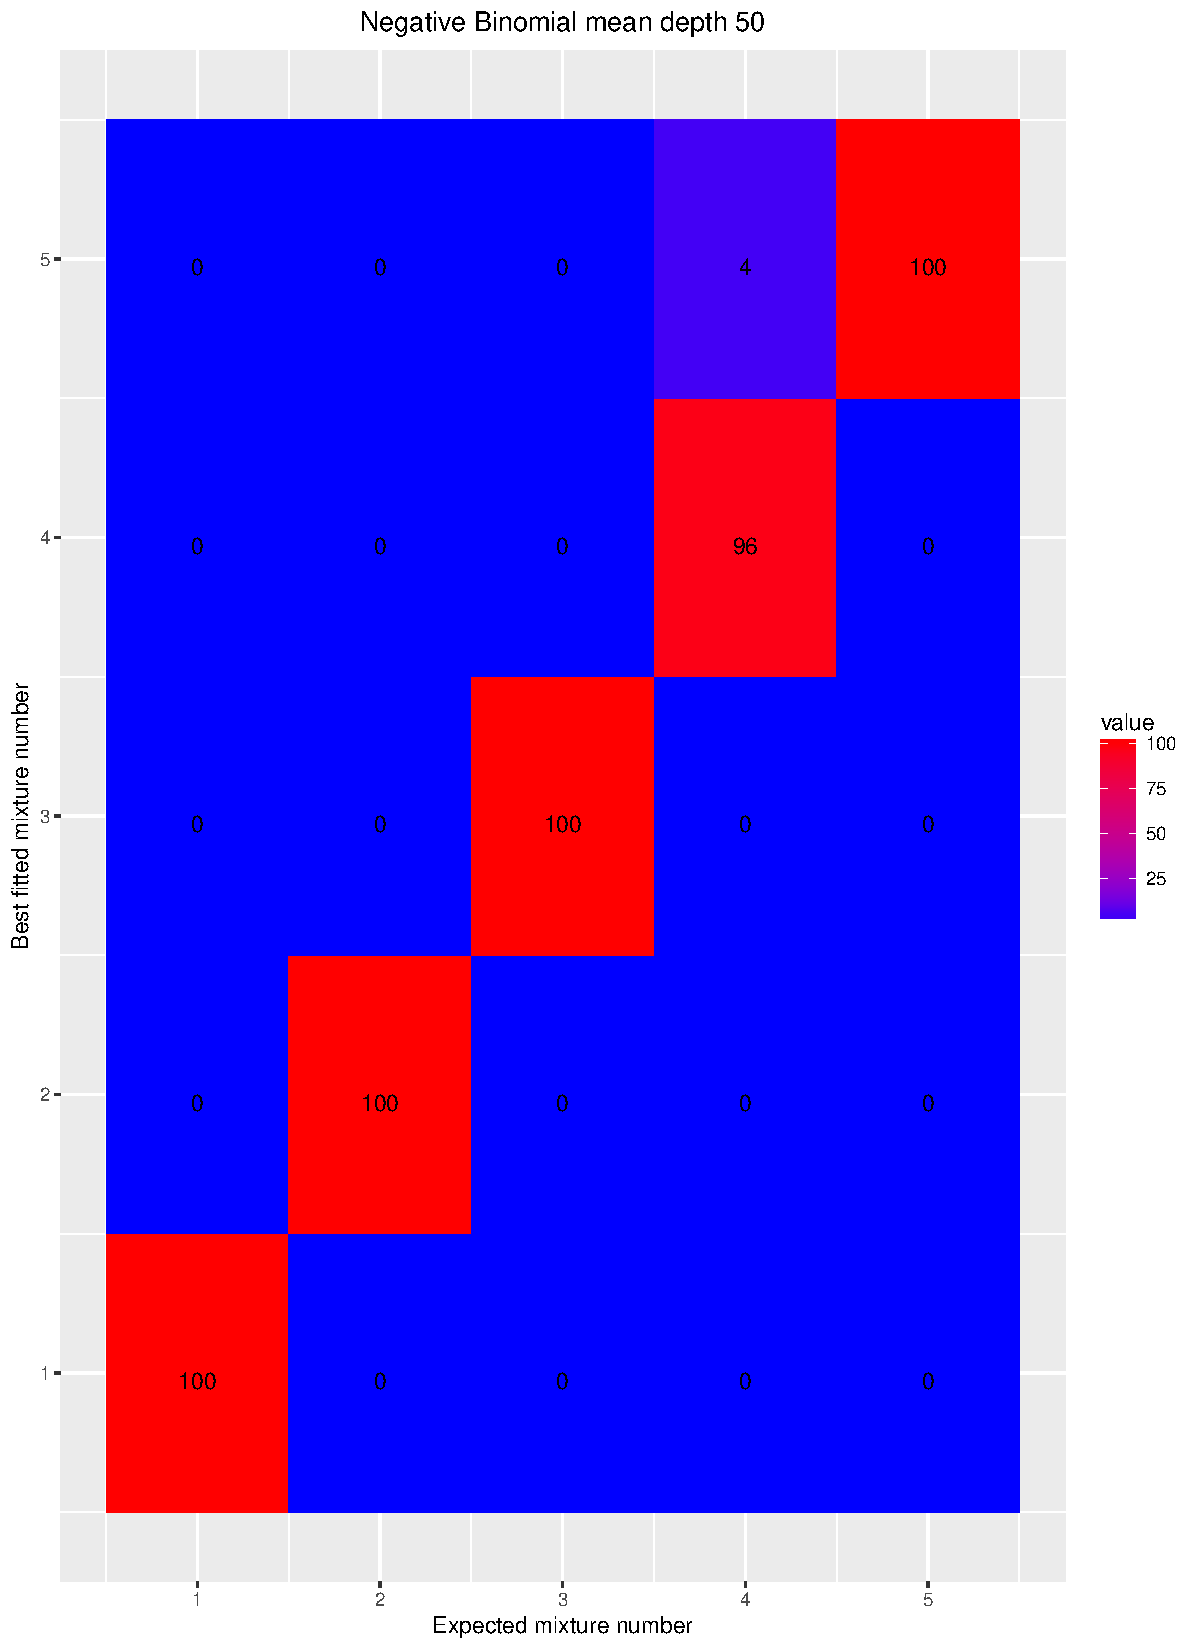
\includegraphics[scale=0.27]{../Results/Second_Analysis/Negative_Binomial_Confusion_Matrix_50.pdf}
% Confusion matrices
\end{center}
\caption{Confusions matrices showing how accurately the mixture of Negative Binomial distribution models predict the amount of CCNV within a genome. Mean depth refers to the mean haploid read depth for each genome.}
\end{figure}

\begin{figure}[H]
\begin{center}
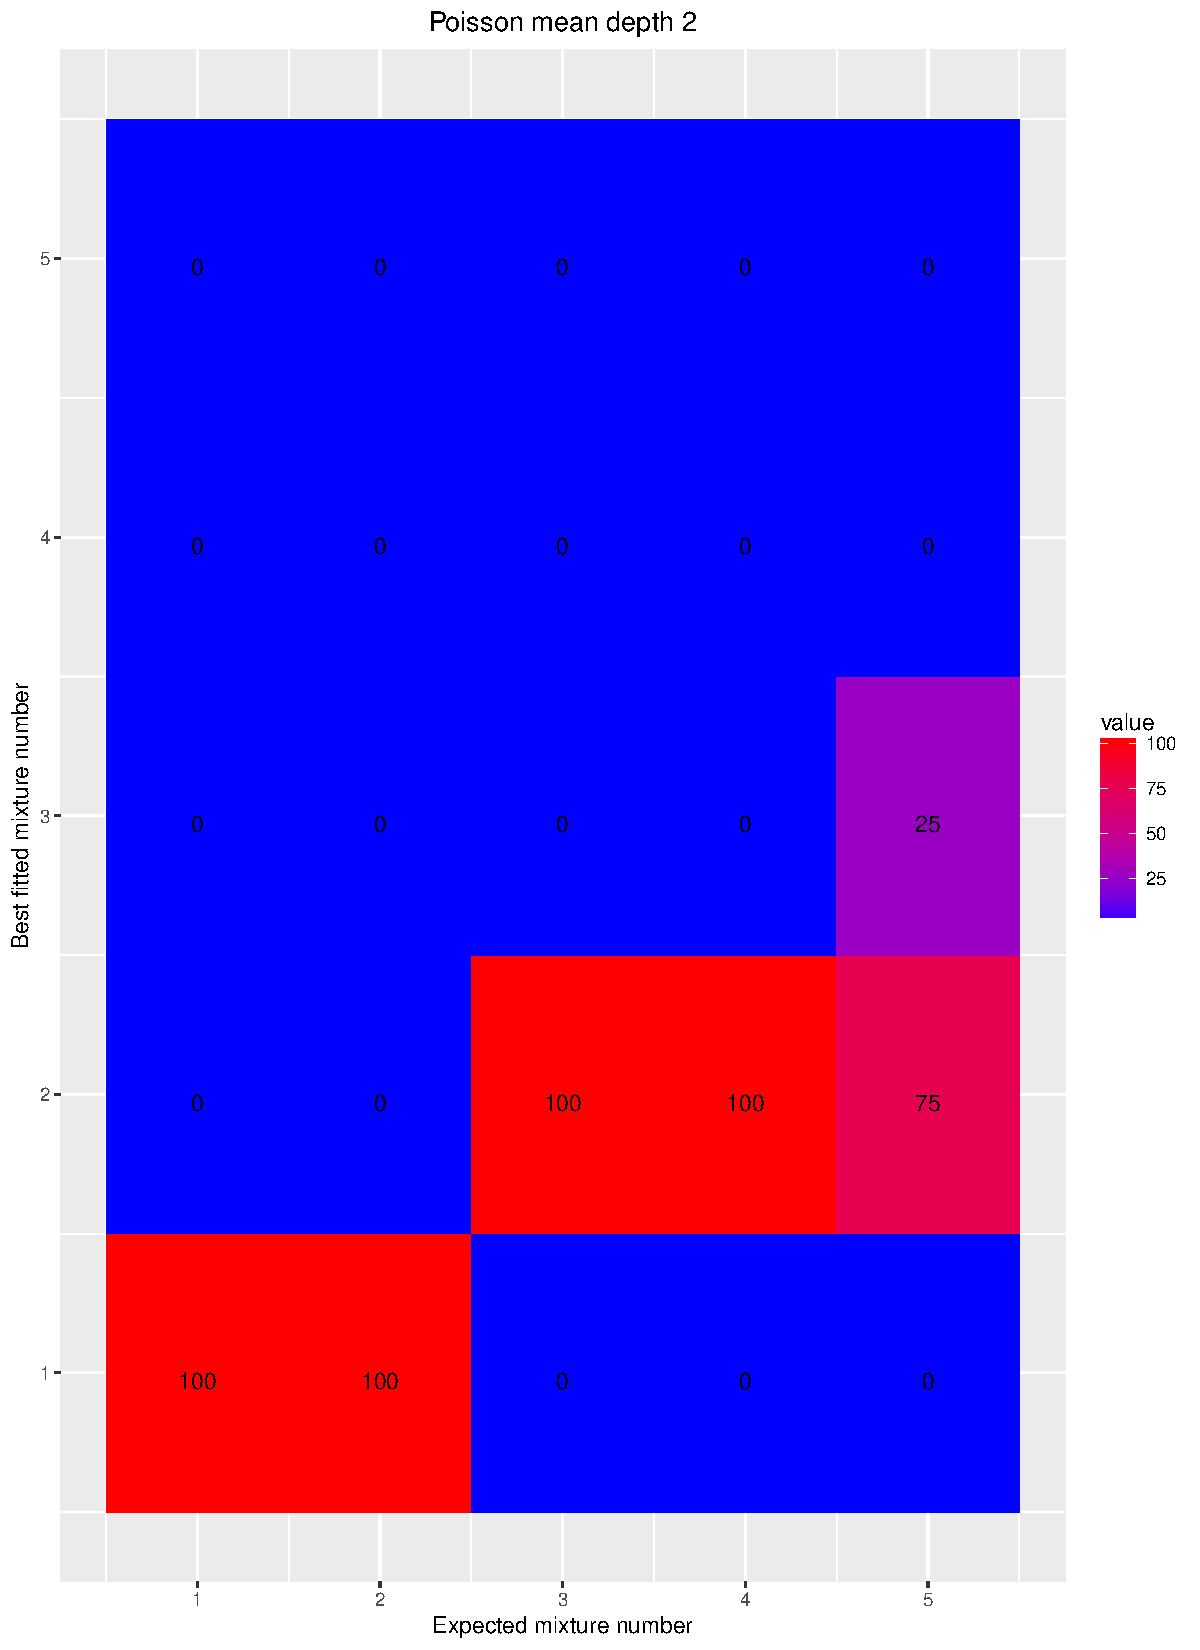
\includegraphics[scale=0.27]{../Results/Second_Analysis/Poisson_Confusion_Matrix_2.pdf}
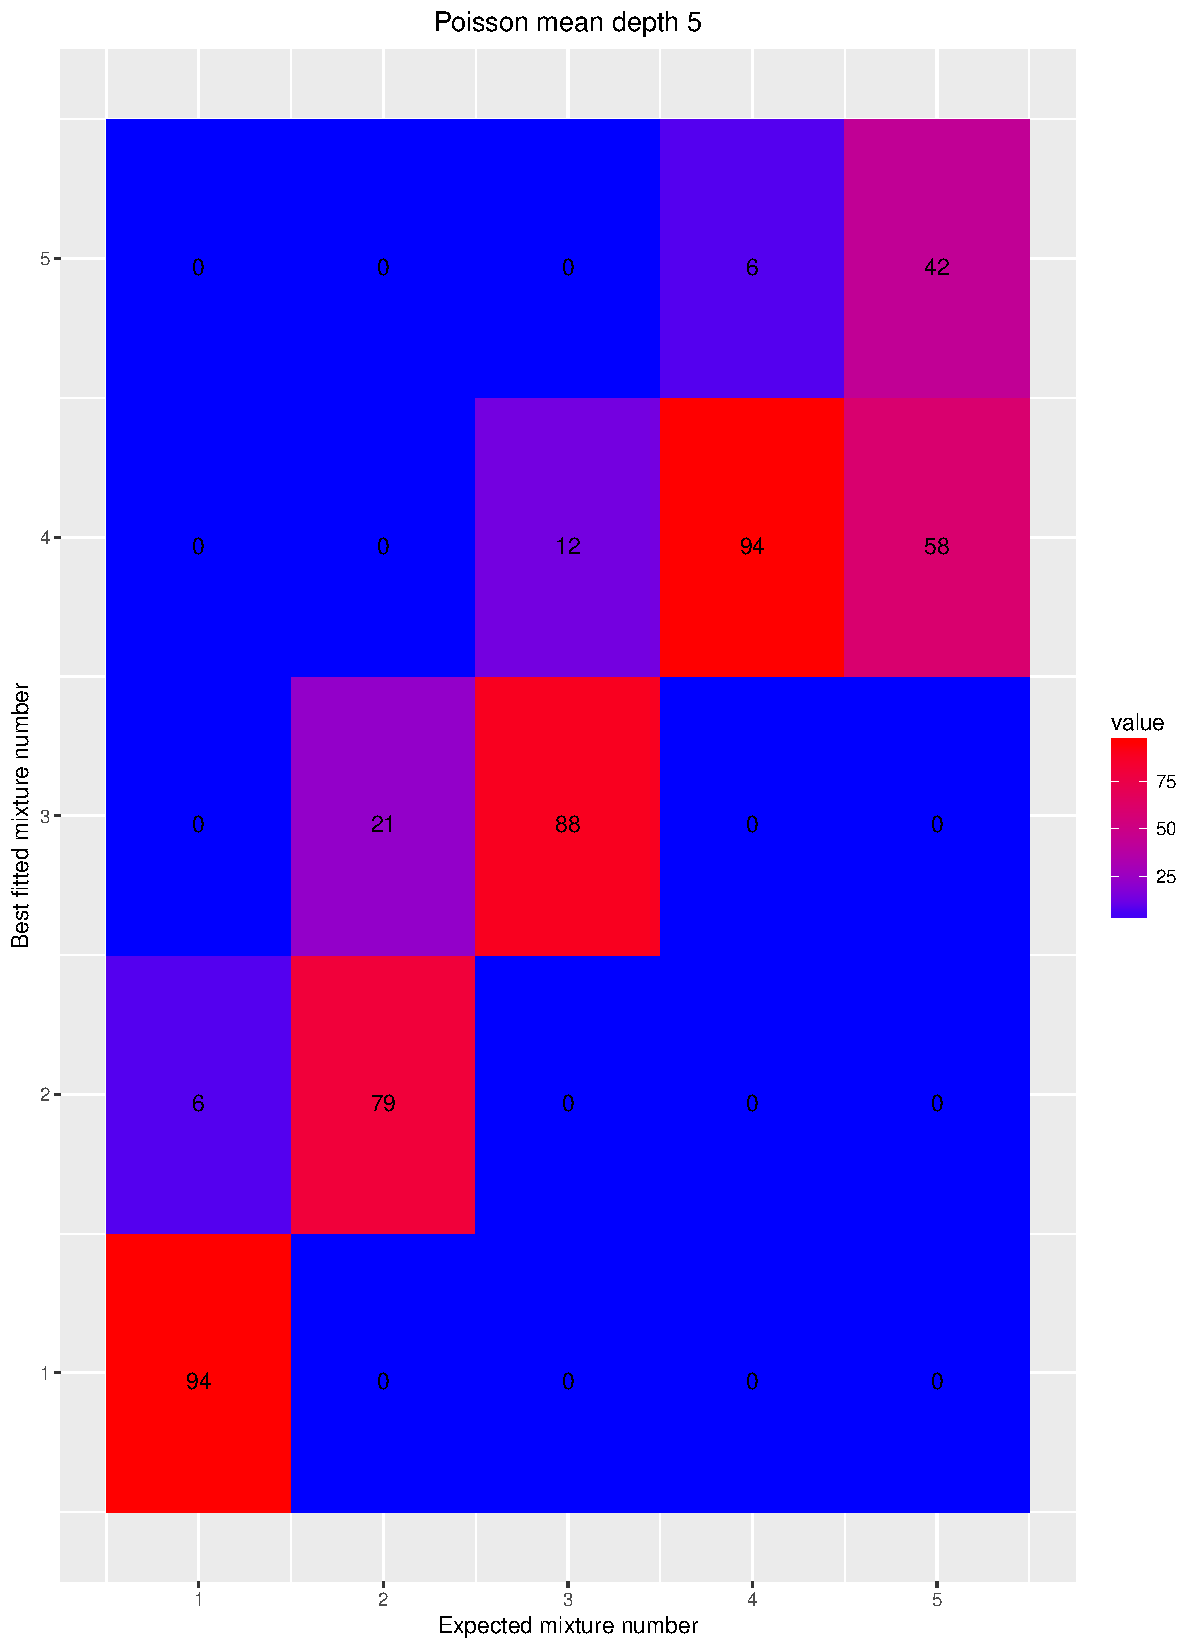
\includegraphics[scale=0.27]{../Results/Second_Analysis/Poisson_Confusion_Matrix_5.pdf}
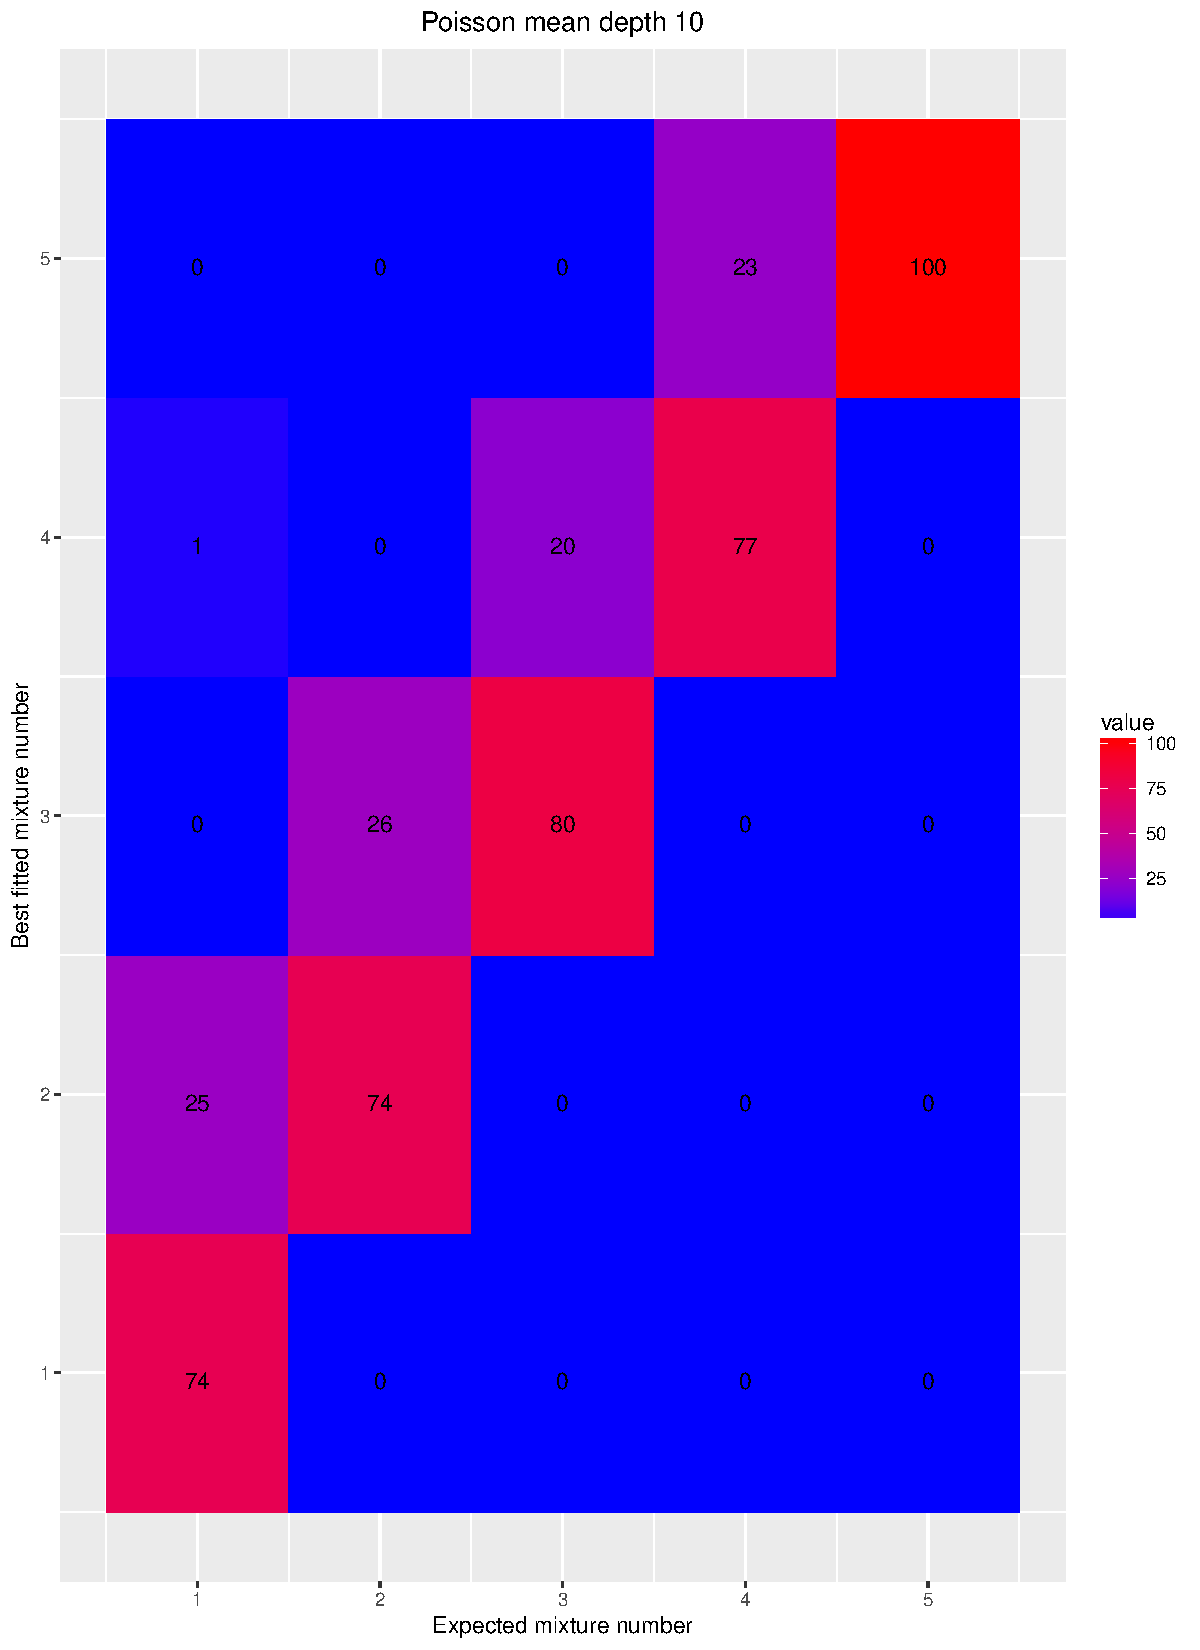
\includegraphics[scale=0.27]{../Results/Second_Analysis/Poisson_Confusion_Matrix_10.pdf}
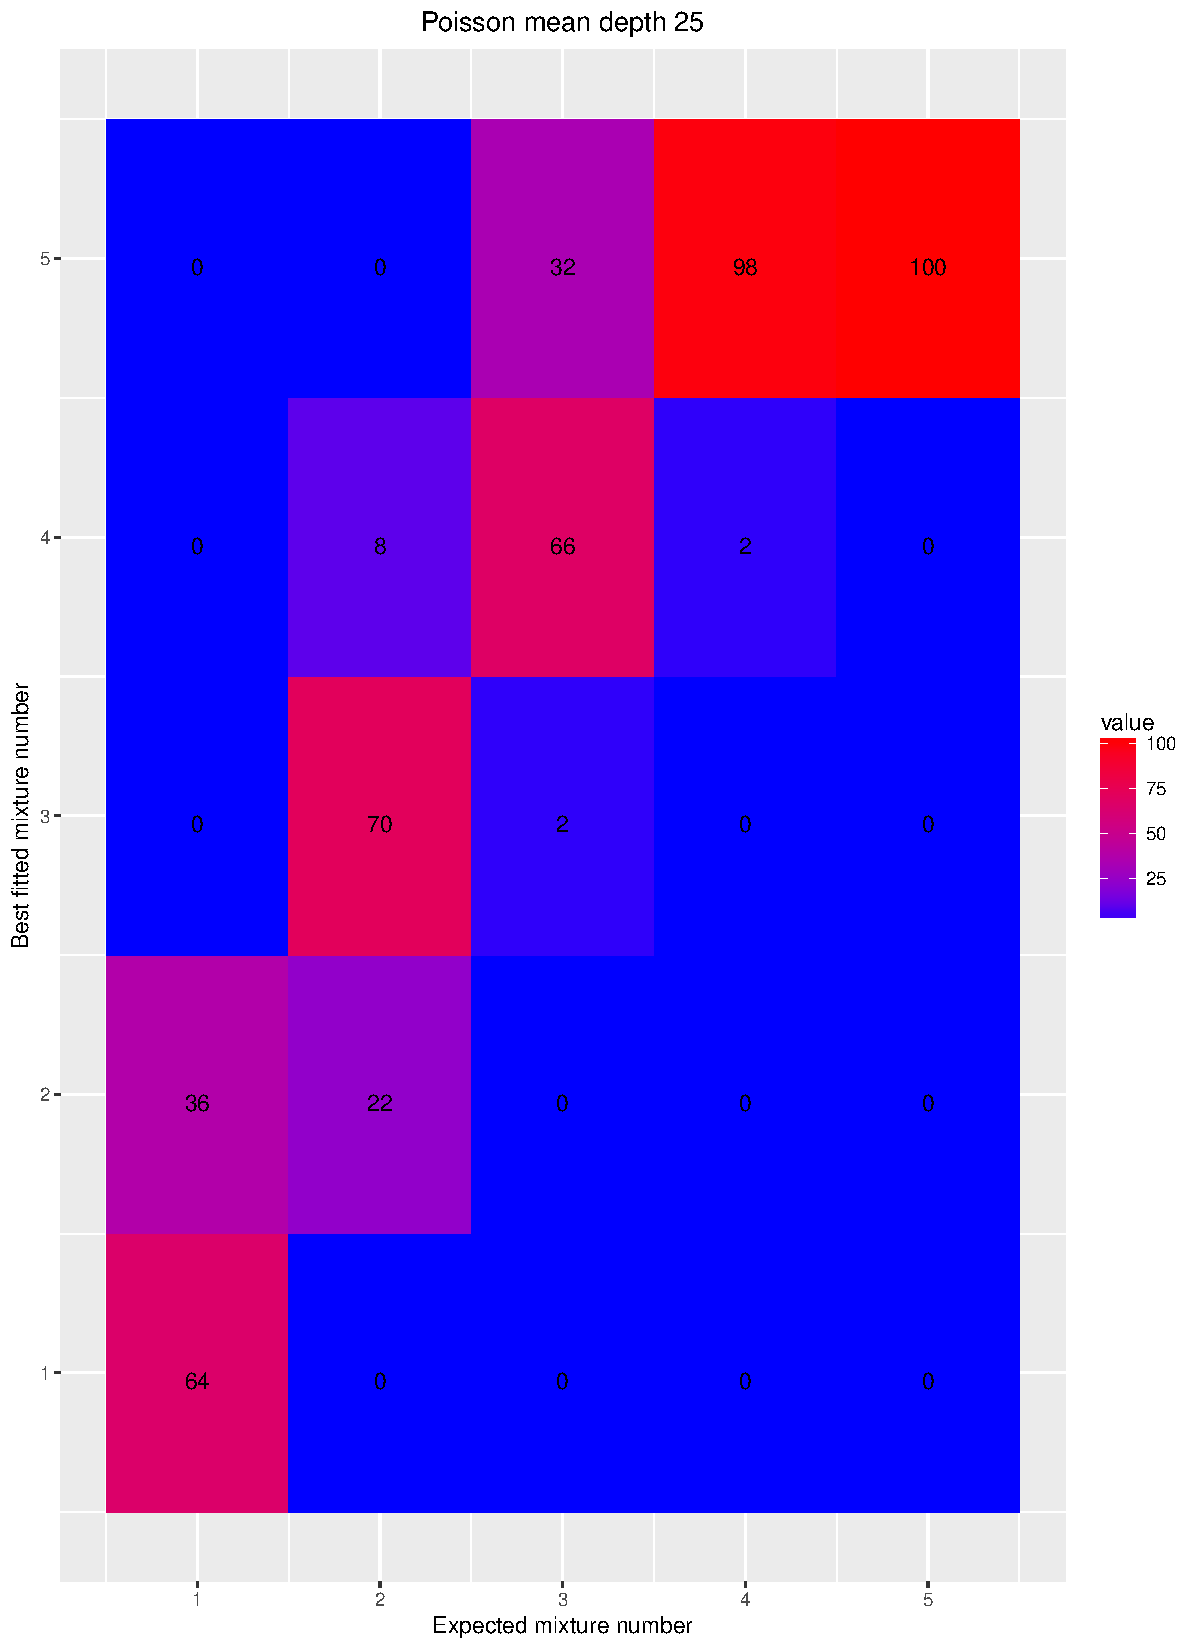
\includegraphics[scale=0.27]{../Results/Second_Analysis/Poisson_Confusion_Matrix_25.pdf}
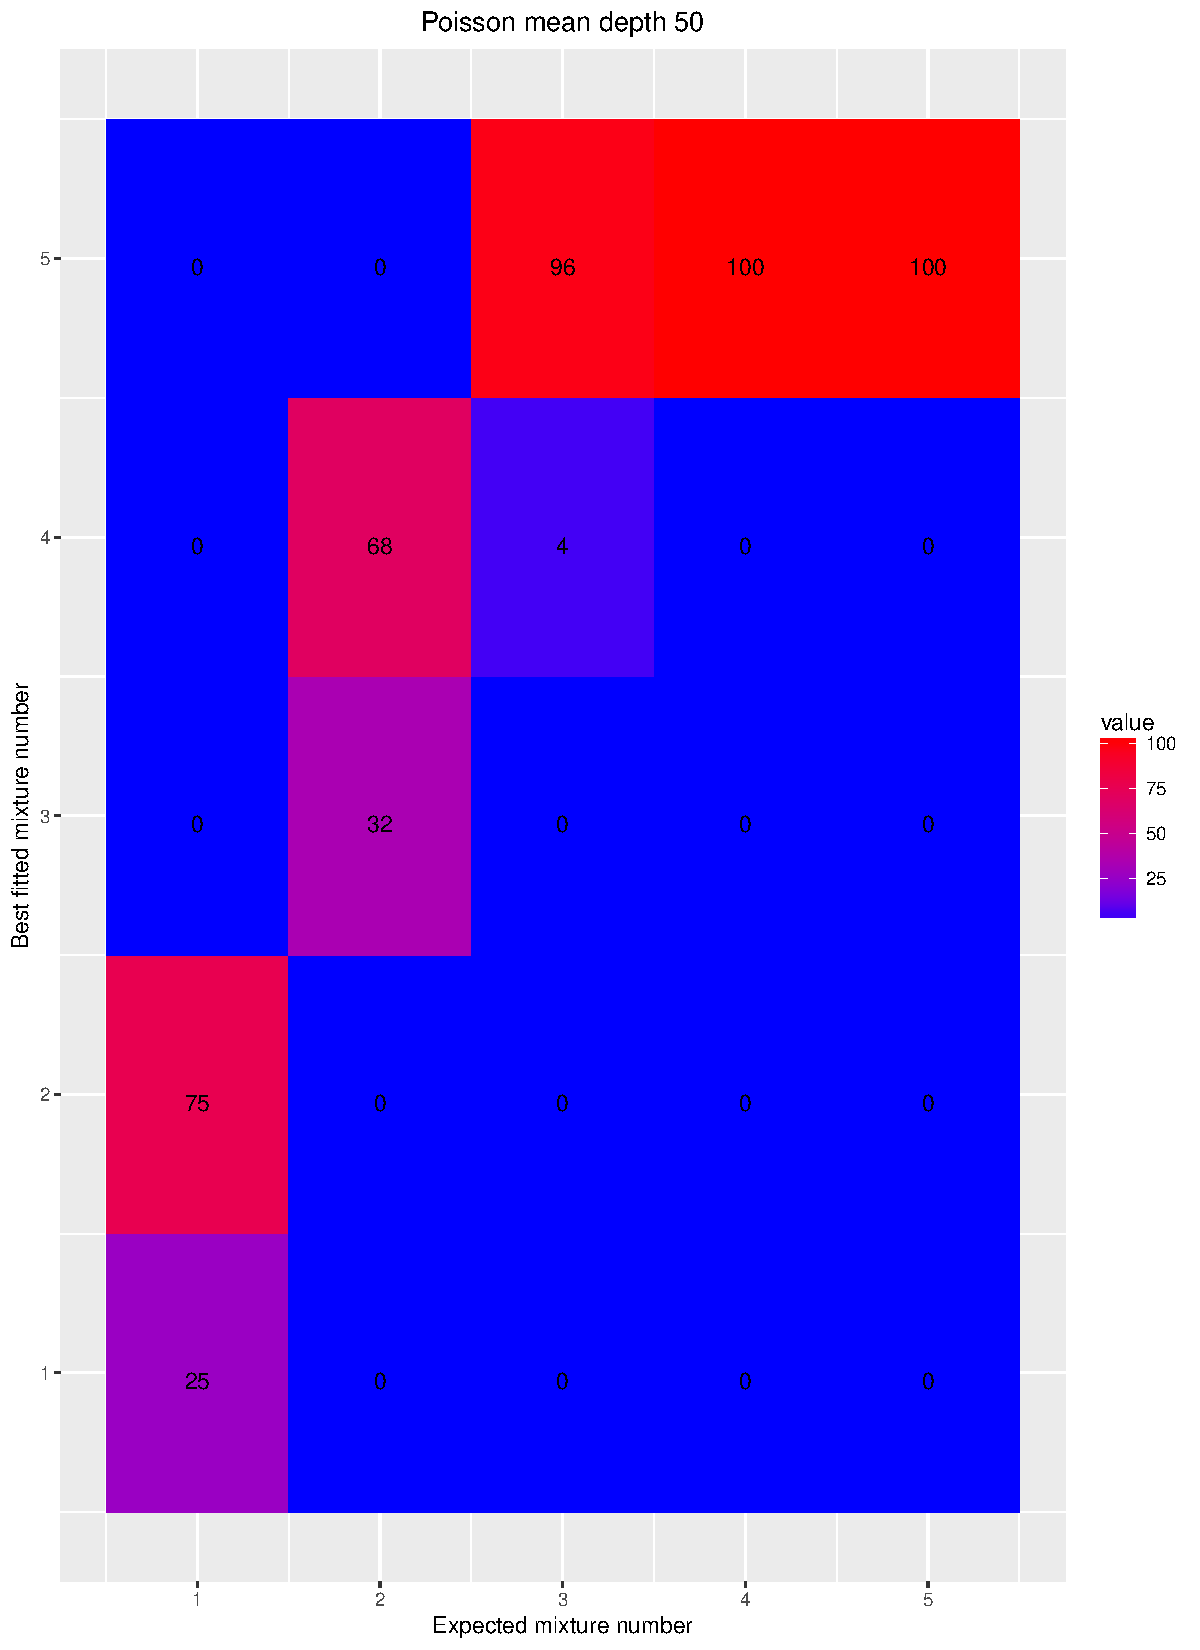
\includegraphics[scale=0.27]{../Results/Second_Analysis/Poisson_Confusion_Matrix_50.pdf}
% Confusion matrices
\end{center}
\caption{Confusions matrices showing how accurately the mixture of Poisson distribution models predict the amount of CCNV within a genome. Mean depth refers to the mean haploid read depth for each genome.}
\end{figure}

\begin{table}[H]
\begin{center}
\caption{RMSD for the predicted number of ploidies for models fitted with the optimal number of curves for each distribution. }
\begin{tabular}{|c||P{4cm}|P{4cm}|}
\hline
\multirow{2}{*}{\textbf{MHRD}} & \multicolumn{2}{|c|}{\textbf{RMSD}} \\
\cline{2-3}
& \textbf{Poisson mixture} & \textbf{Negative Binomial mixture} \\
\hline
\hline
\textbf{2} & 1.658 & 2.139 \\
\hline
\textbf{5} & 0.454 & 1.050 \\
\hline
\textbf{10} & 0.454 & 0.424 \\
\hline
\textbf{25} & 0.927 & 0.110 \\
\hline
\textbf{50} & 1.317 & 0.089 \\
\hline
\hline
\end{tabular}
\end{center}
\end{table}

Genomes generated with randomly assigned ploidy levels show a similar effect as those formed in the genomes with stepped ploidies. Again the Poisson mixture performs better at very low depths whilst the Negative Binomial gives improved accuracy at higher read depths. Overall the total error is also lower for both distributions at low depths than it was for the stepped ploidies but this error increases more emphatically for the random genomes and produces overall worse fits at the higher depths (Table 3). 

%\begin{figure}[H]
%\begin{center}
%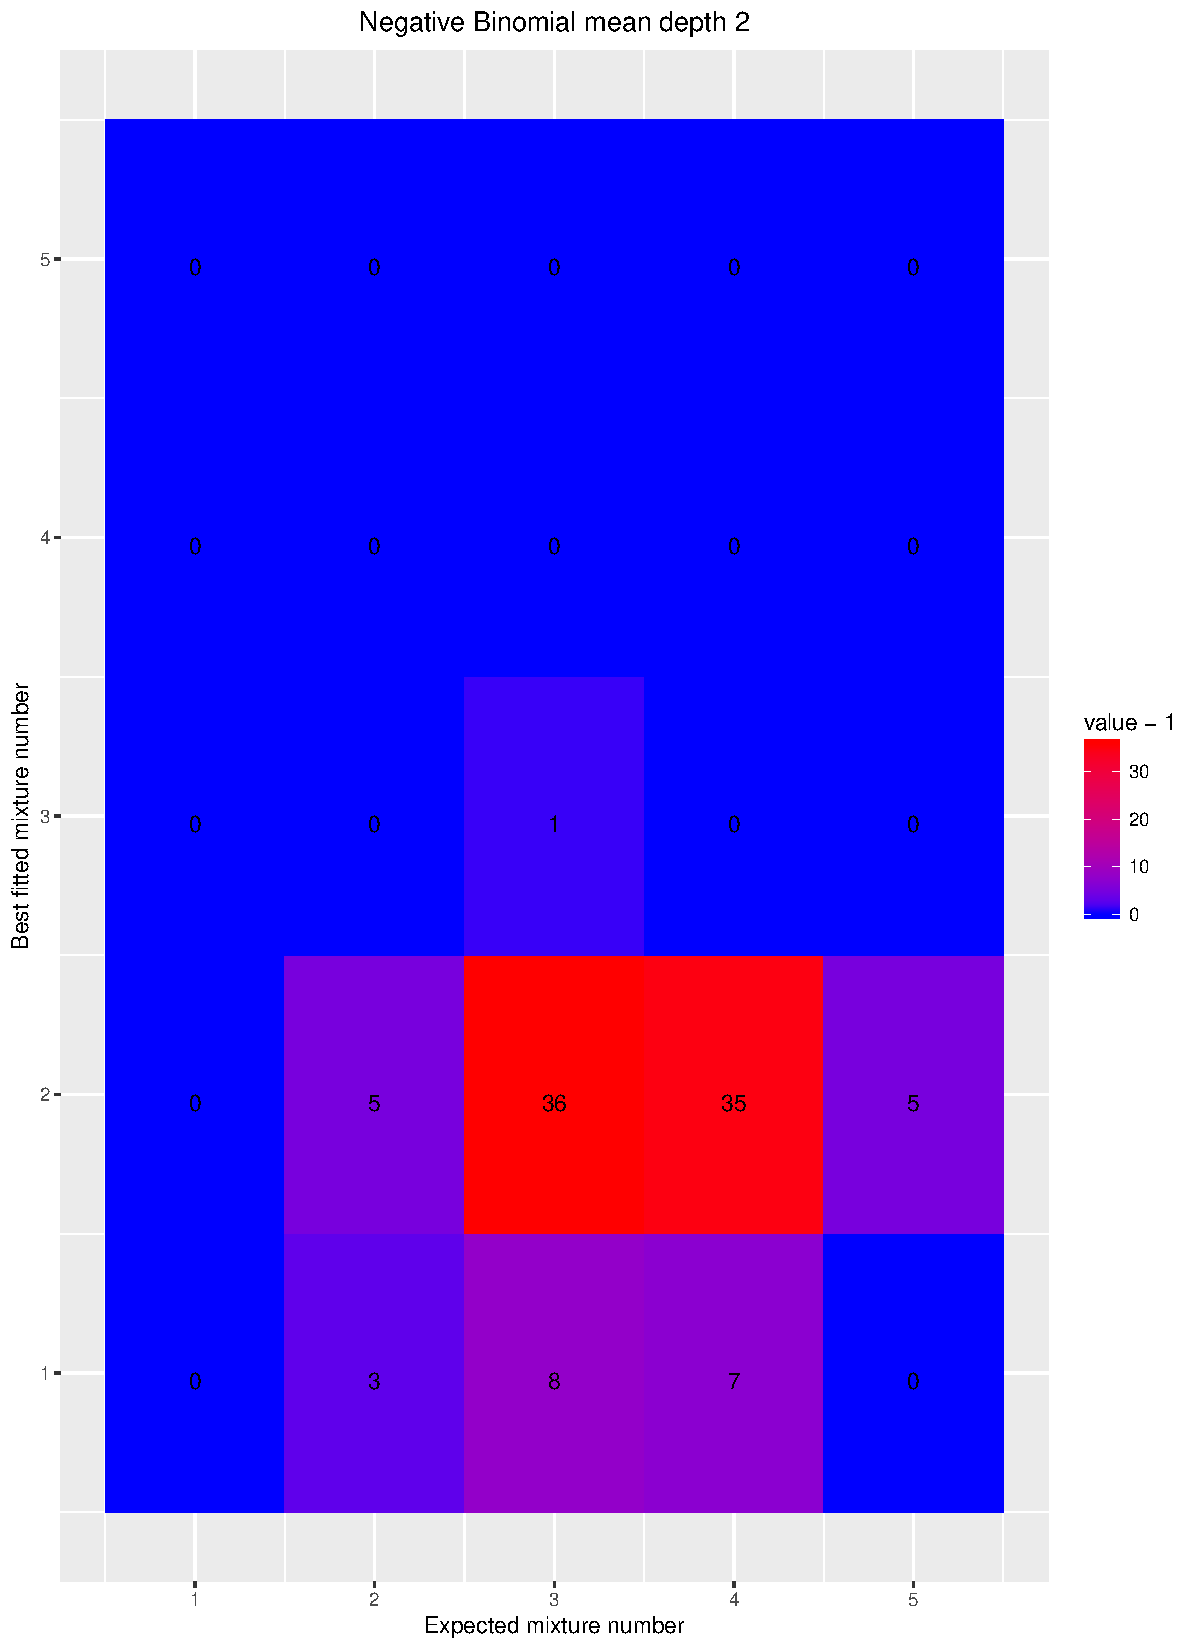
\includegraphics[scale=0.27]{../Results/Third_Analysis/Negative_Binomial_Confusion_Matrix_2.pdf}
%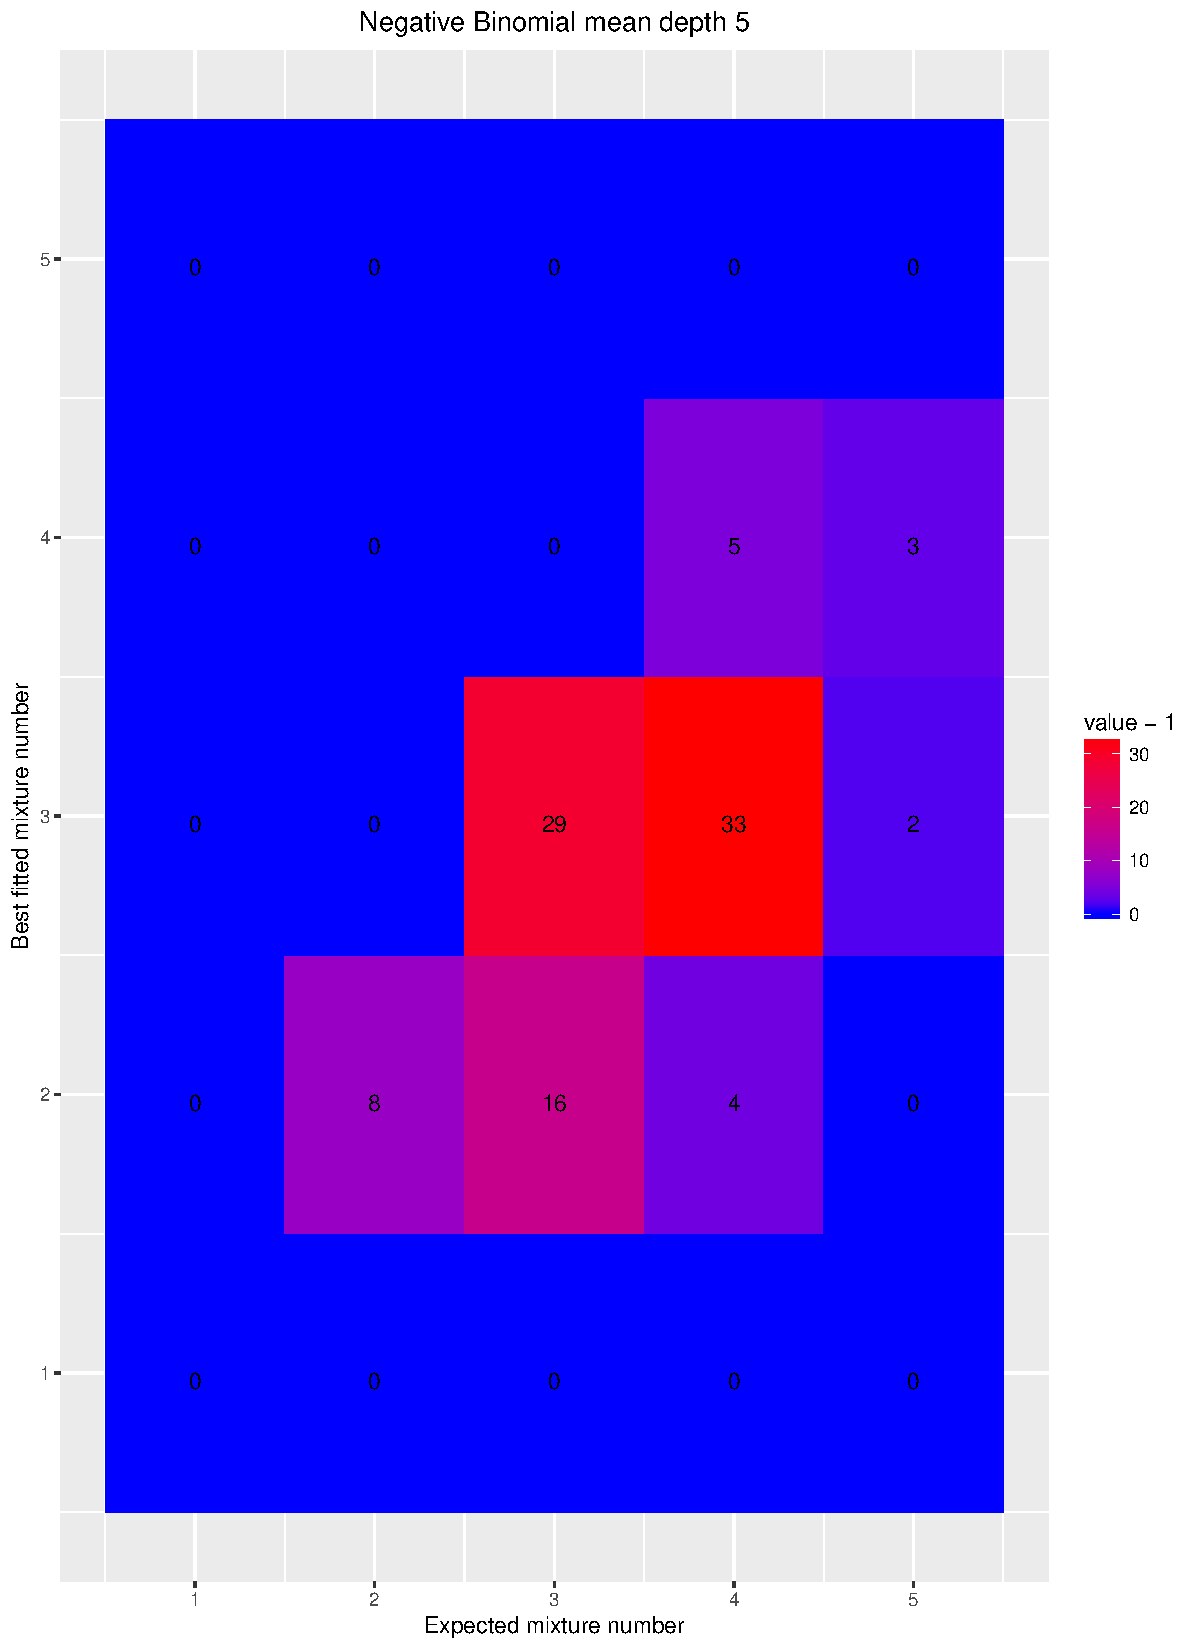
\includegraphics[scale=0.27]{../Results/Third_Analysis/Negative_Binomial_Confusion_Matrix_5.pdf}
%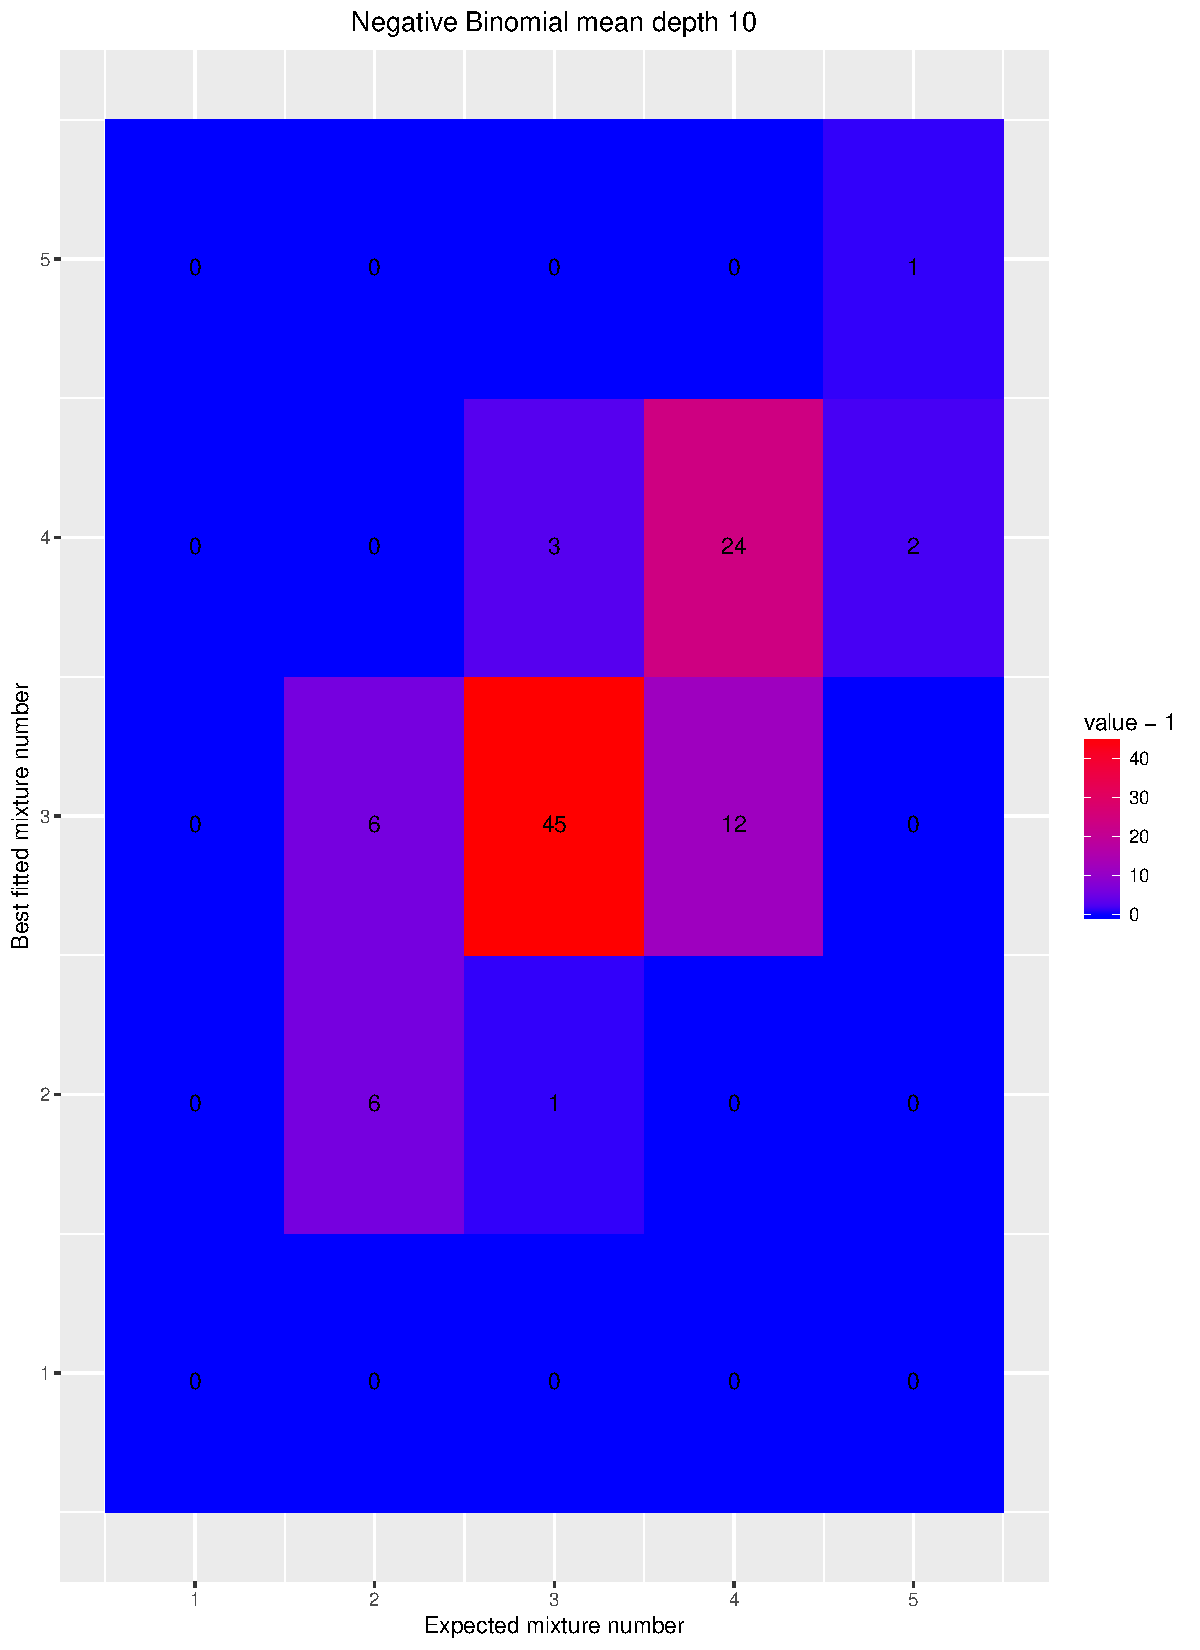
\includegraphics[scale=0.27]{../Results/Third_Analysis/Negative_Binomial_Confusion_Matrix_10.pdf}
%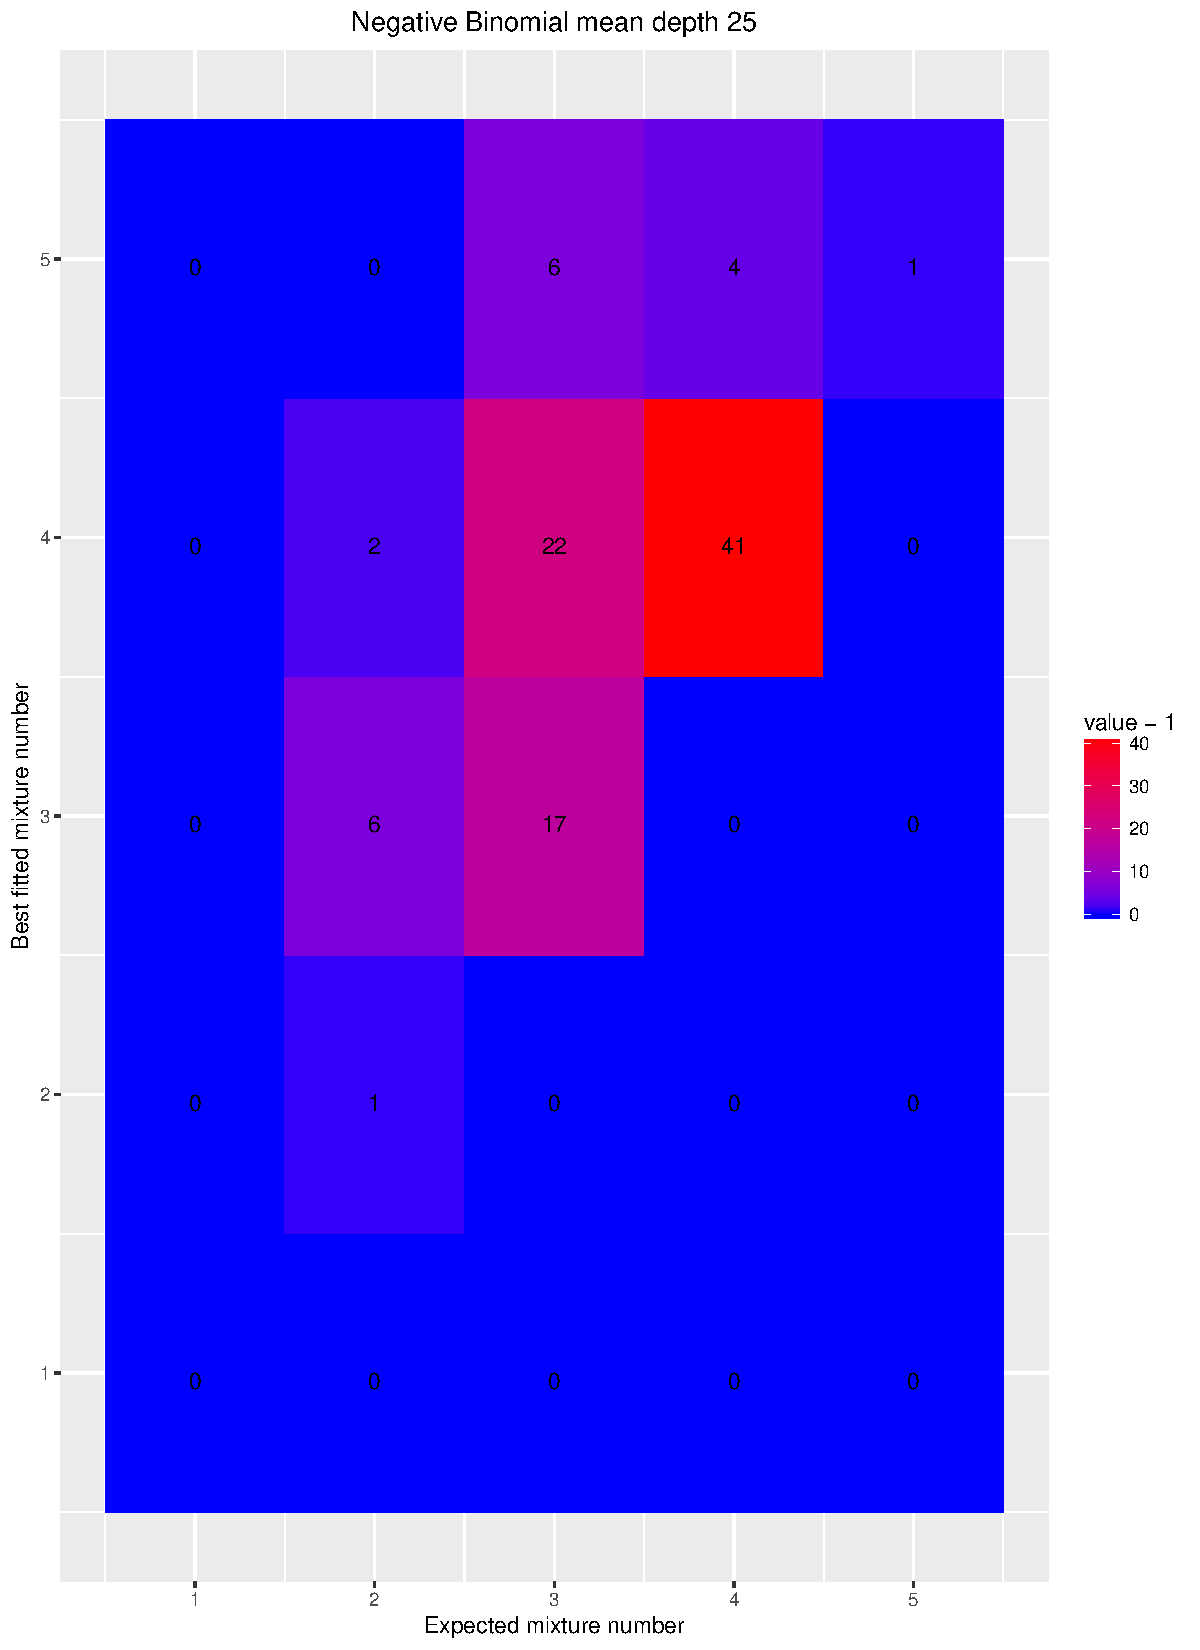
\includegraphics[scale=0.27]{../Results/Third_Analysis/Negative_Binomial_Confusion_Matrix_25.pdf}
%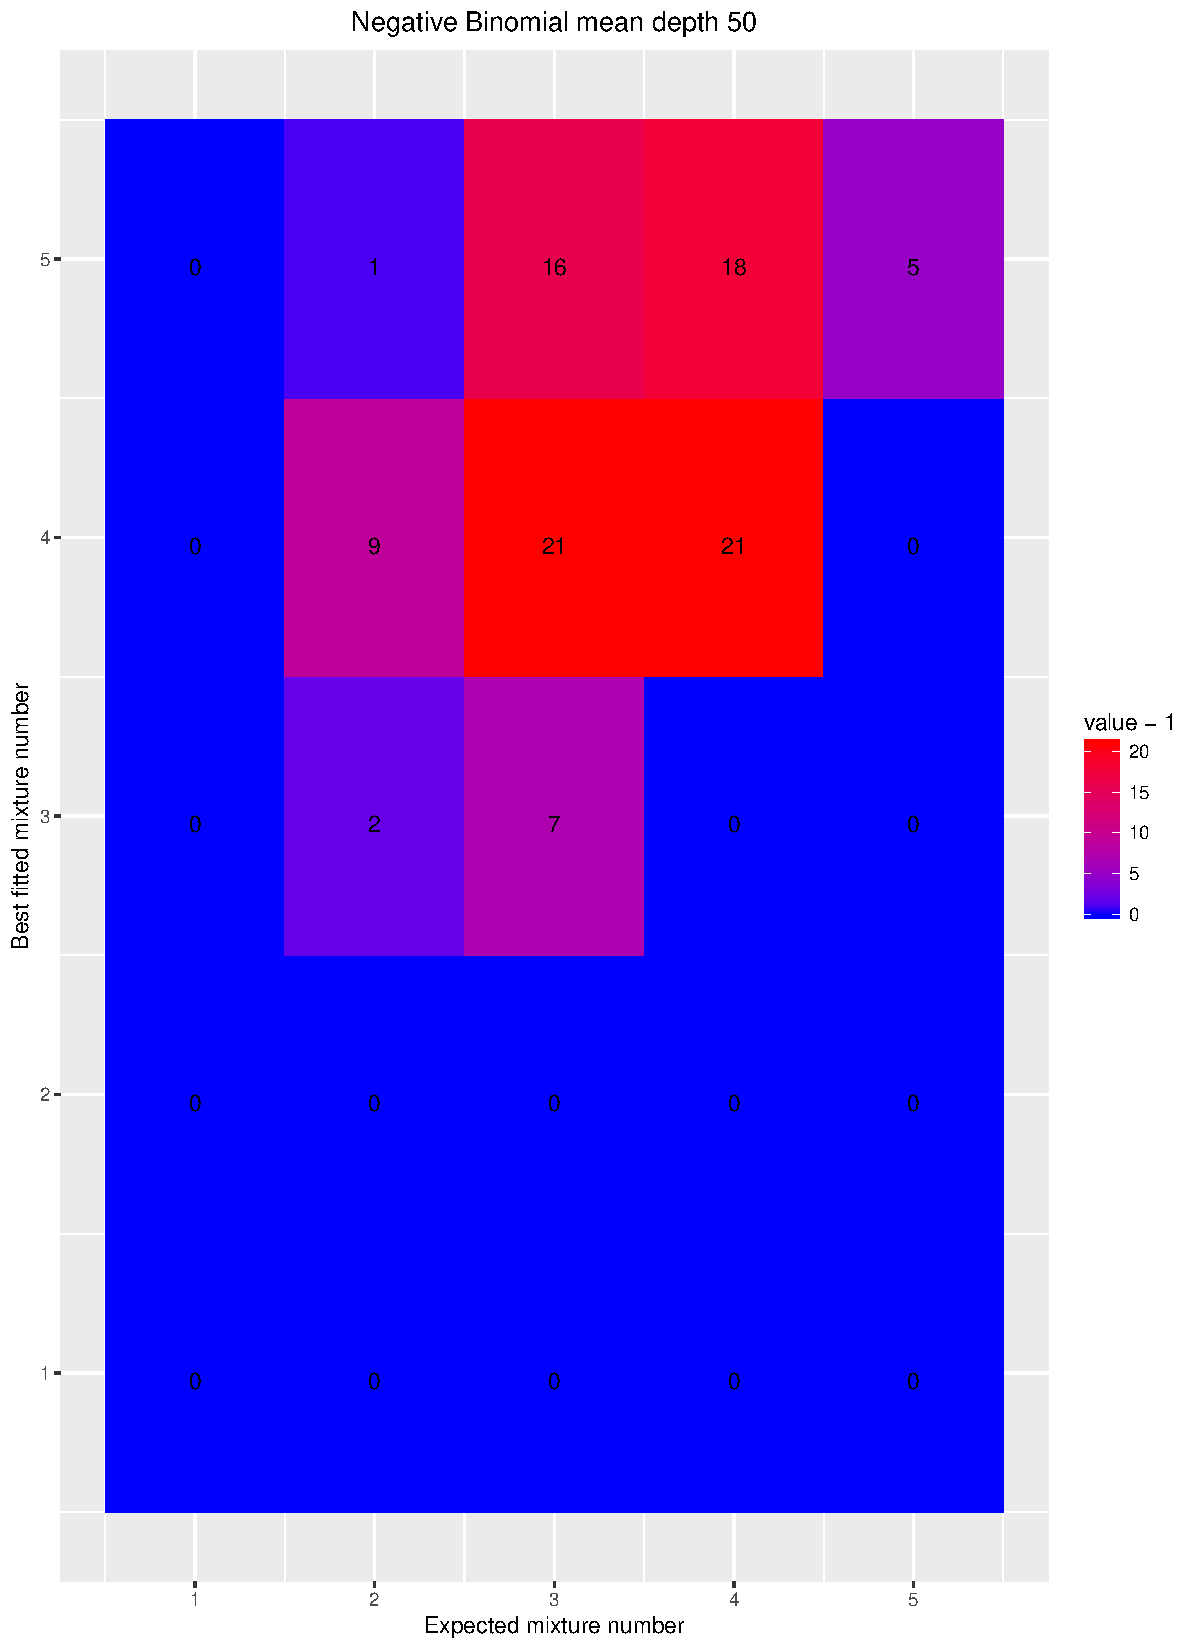
\includegraphics[scale=0.27]{../Results/Third_Analysis/Negative_Binomial_Confusion_Matrix_50.pdf}
%\caption{Confusion matrices of the optimal number of curves in the fitted models for the Negative Binomial distribution for 100 genomes at each mean haploid read depth, each generated with random ploidy levels.}
%% Confusion matrices
%\end{center}
%\end{figure}
%
%\begin{figure}[H]
%\begin{center}
%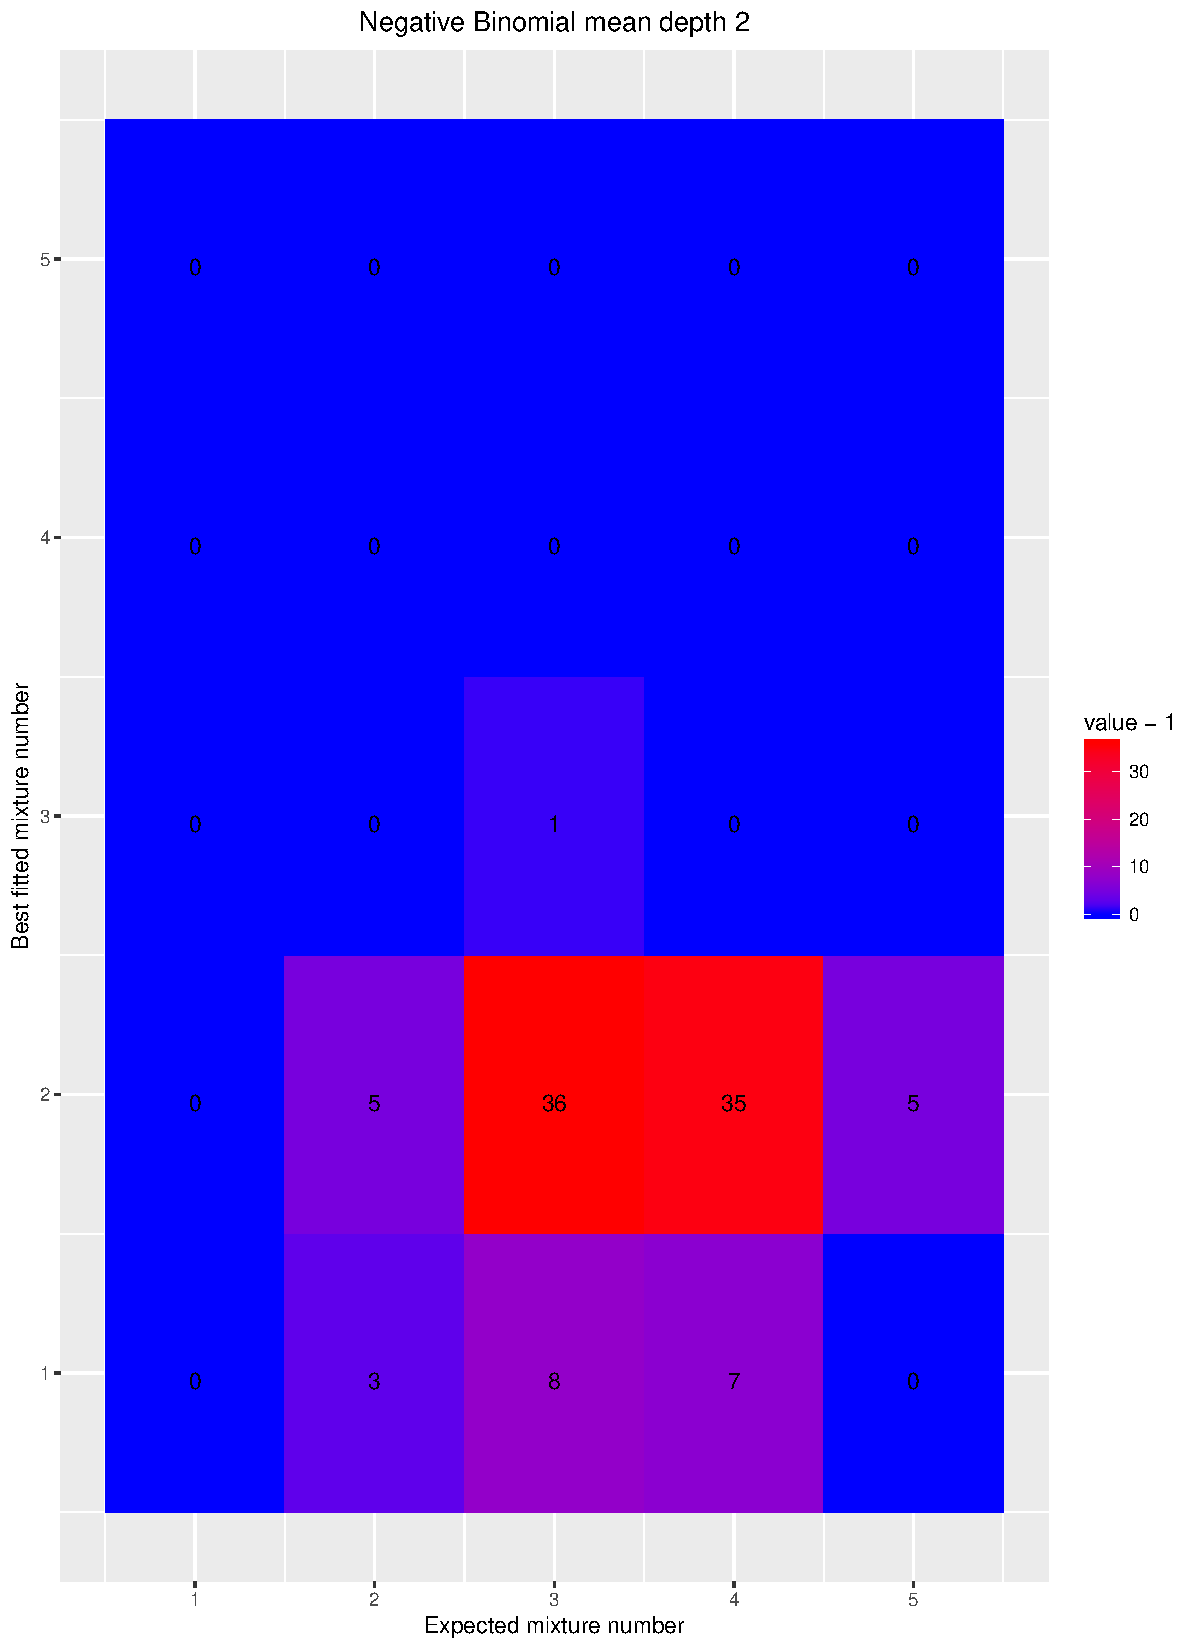
\includegraphics[scale=0.27]{../Results/Third_Analysis/Negative_Binomial_Confusion_Matrix_2.pdf}
%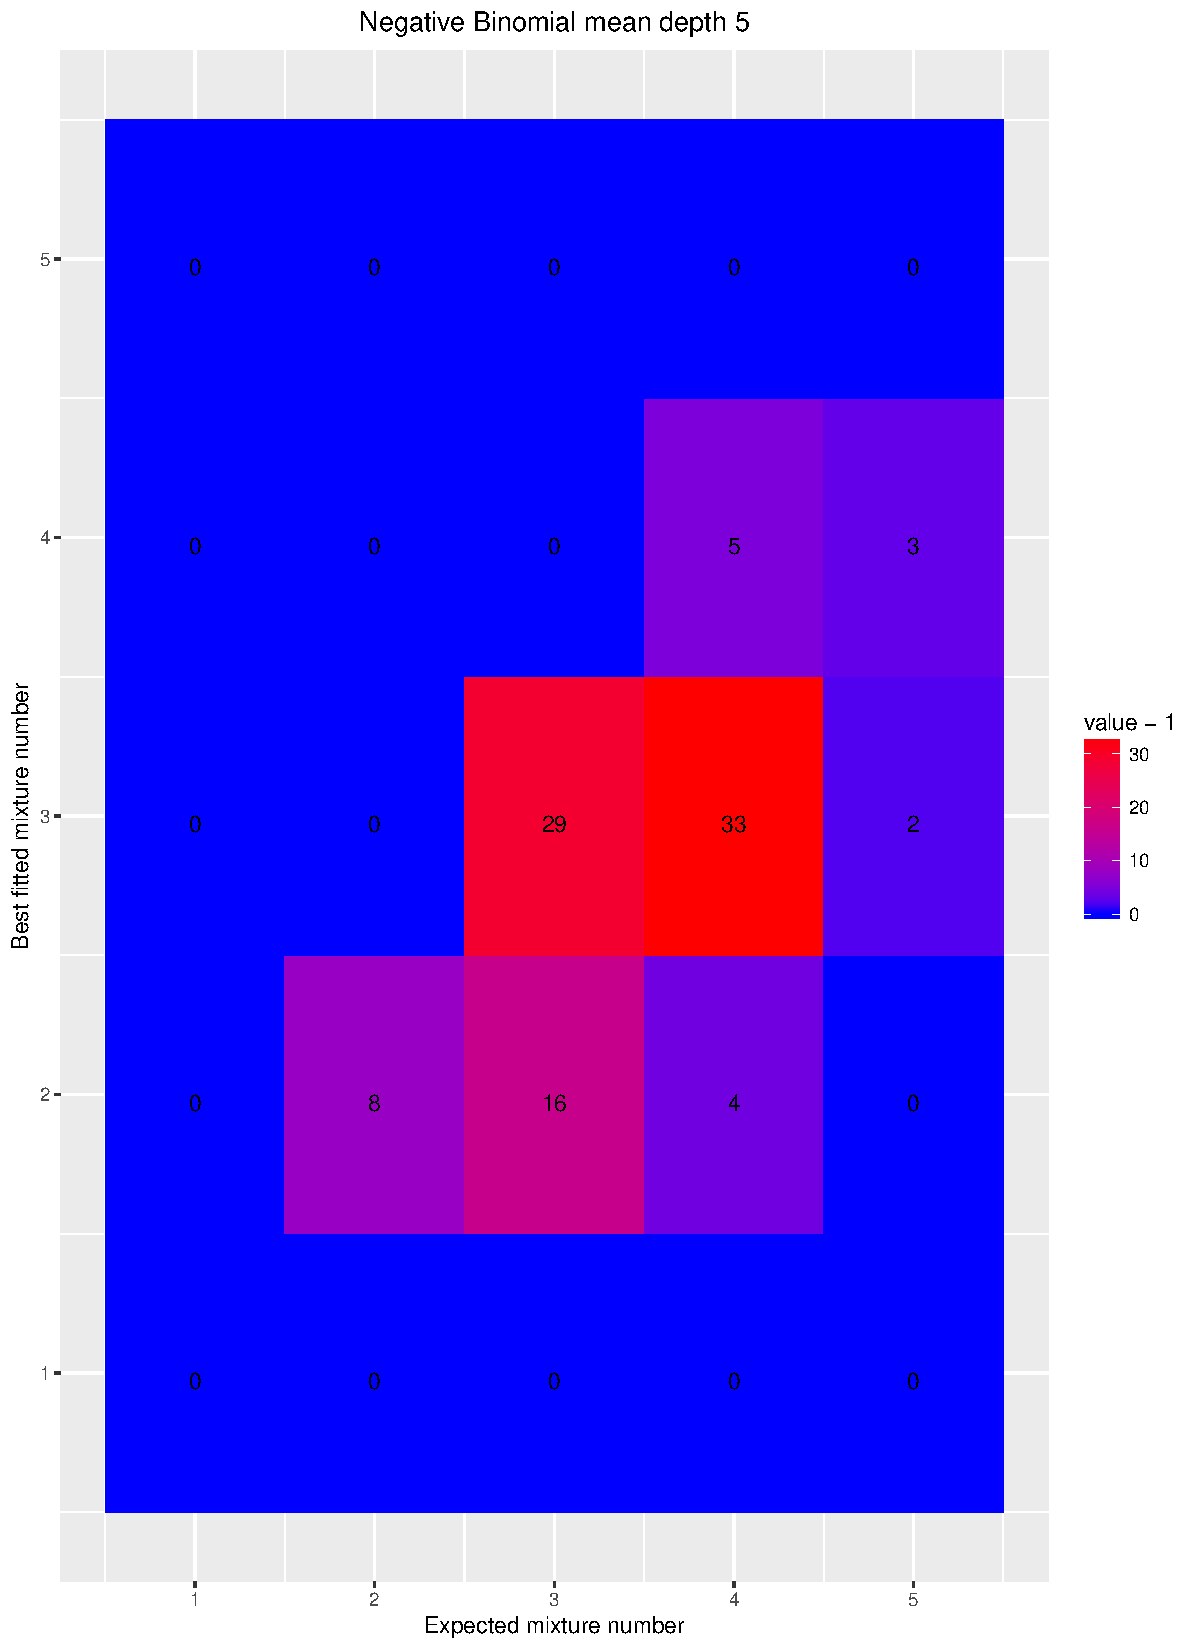
\includegraphics[scale=0.27]{../Results/Third_Analysis/Negative_Binomial_Confusion_Matrix_5.pdf}
%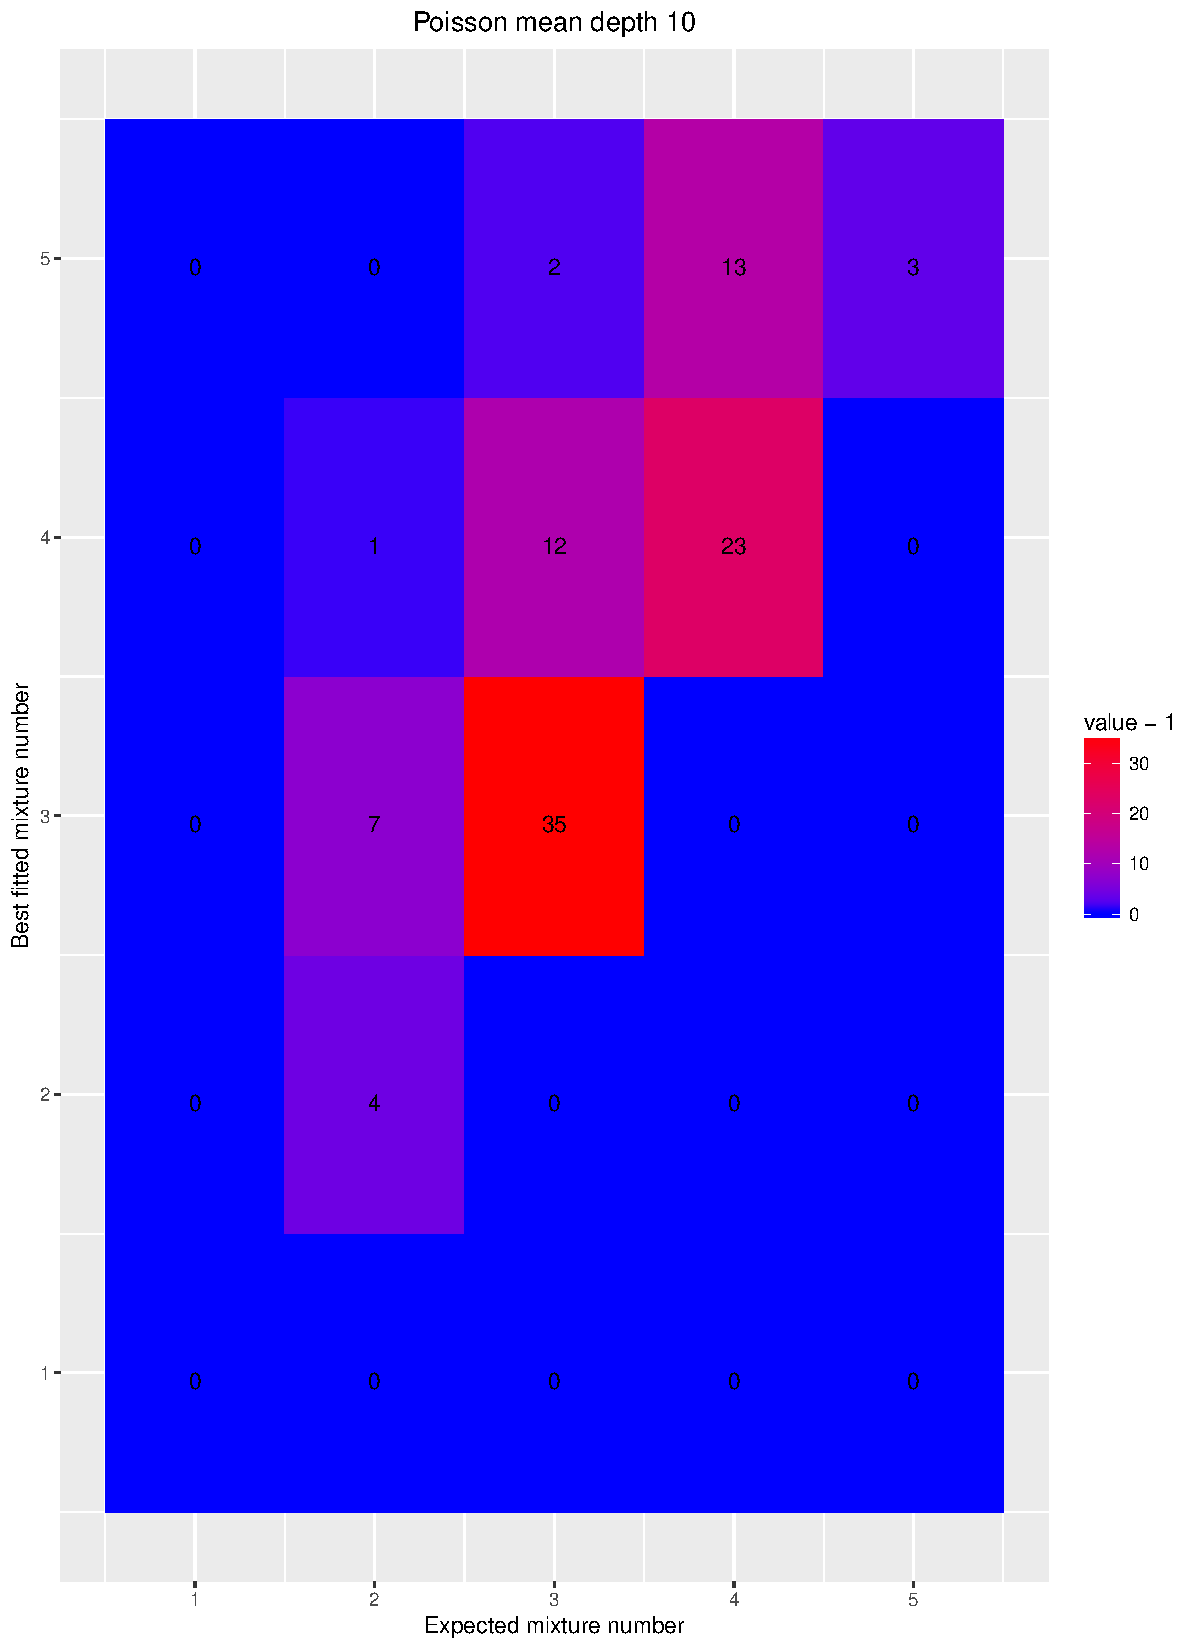
\includegraphics[scale=0.27]{../Results/Third_Analysis/Poisson_Confusion_Matrix_10.pdf}
%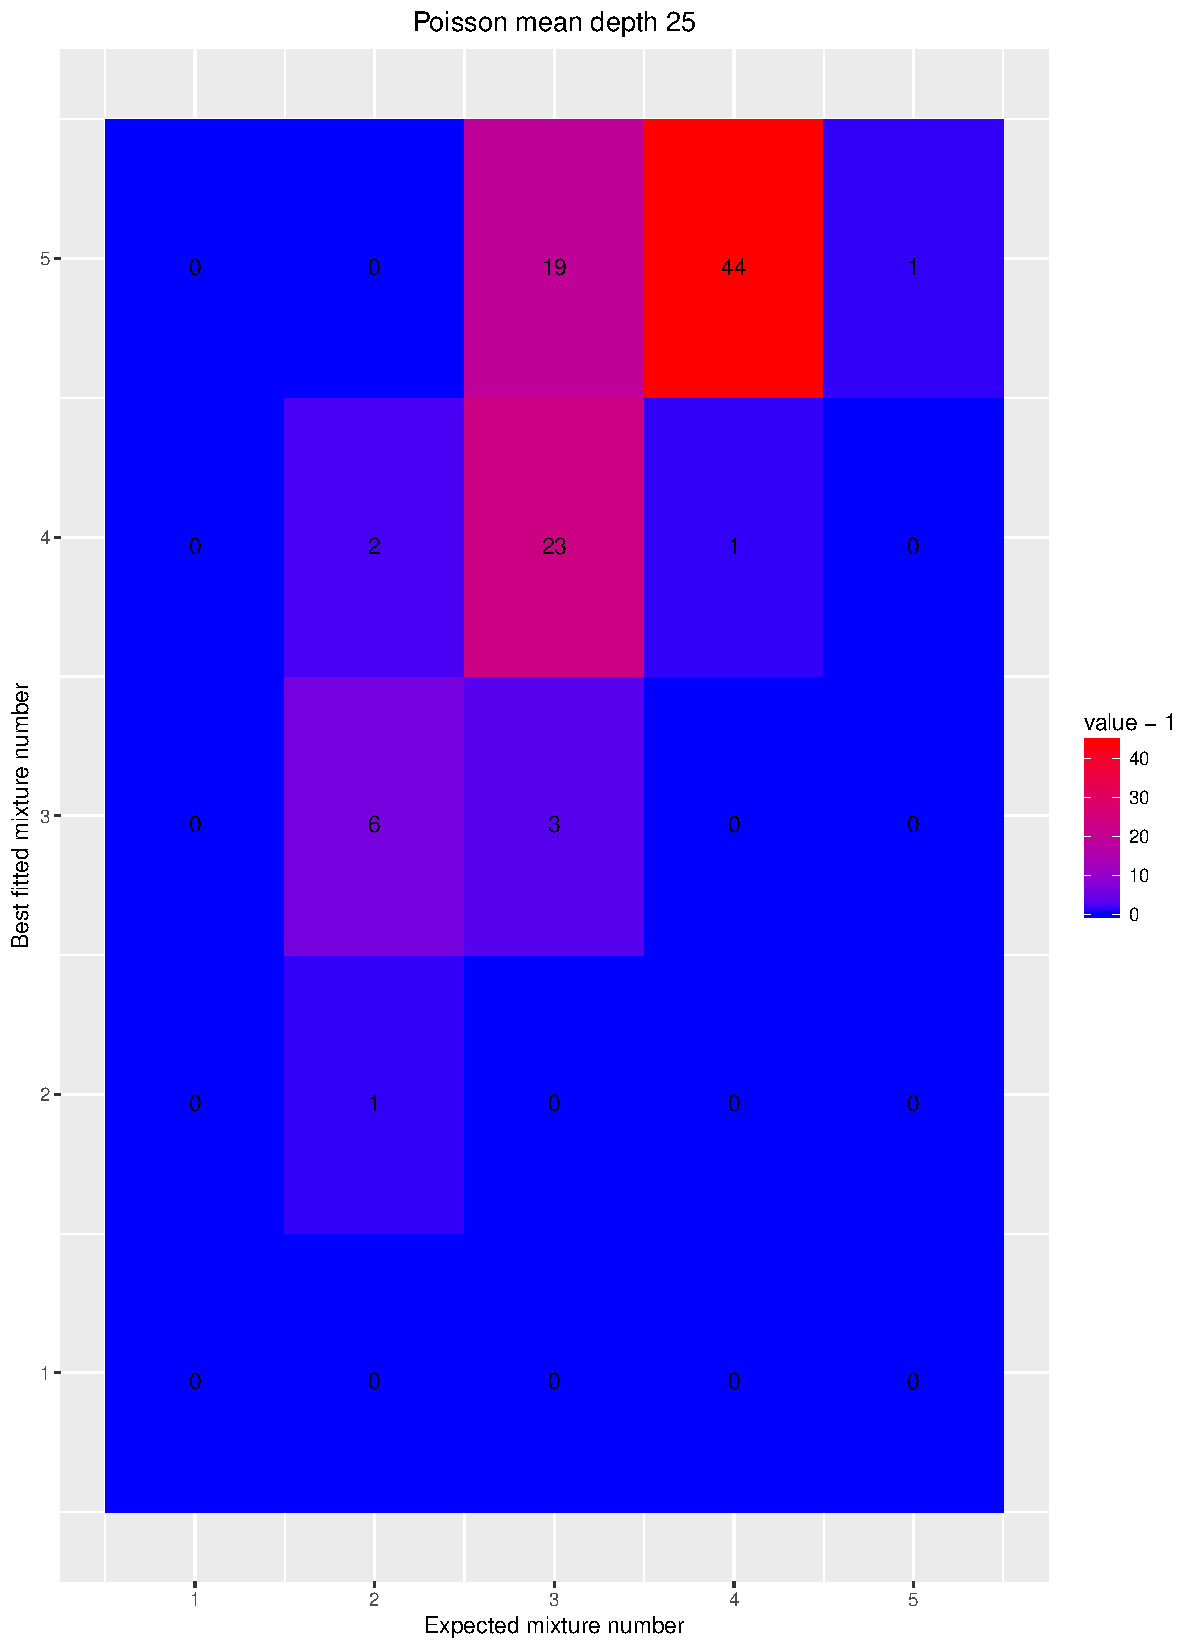
\includegraphics[scale=0.27]{../Results/Third_Analysis/Poisson_Confusion_Matrix_25.pdf}
%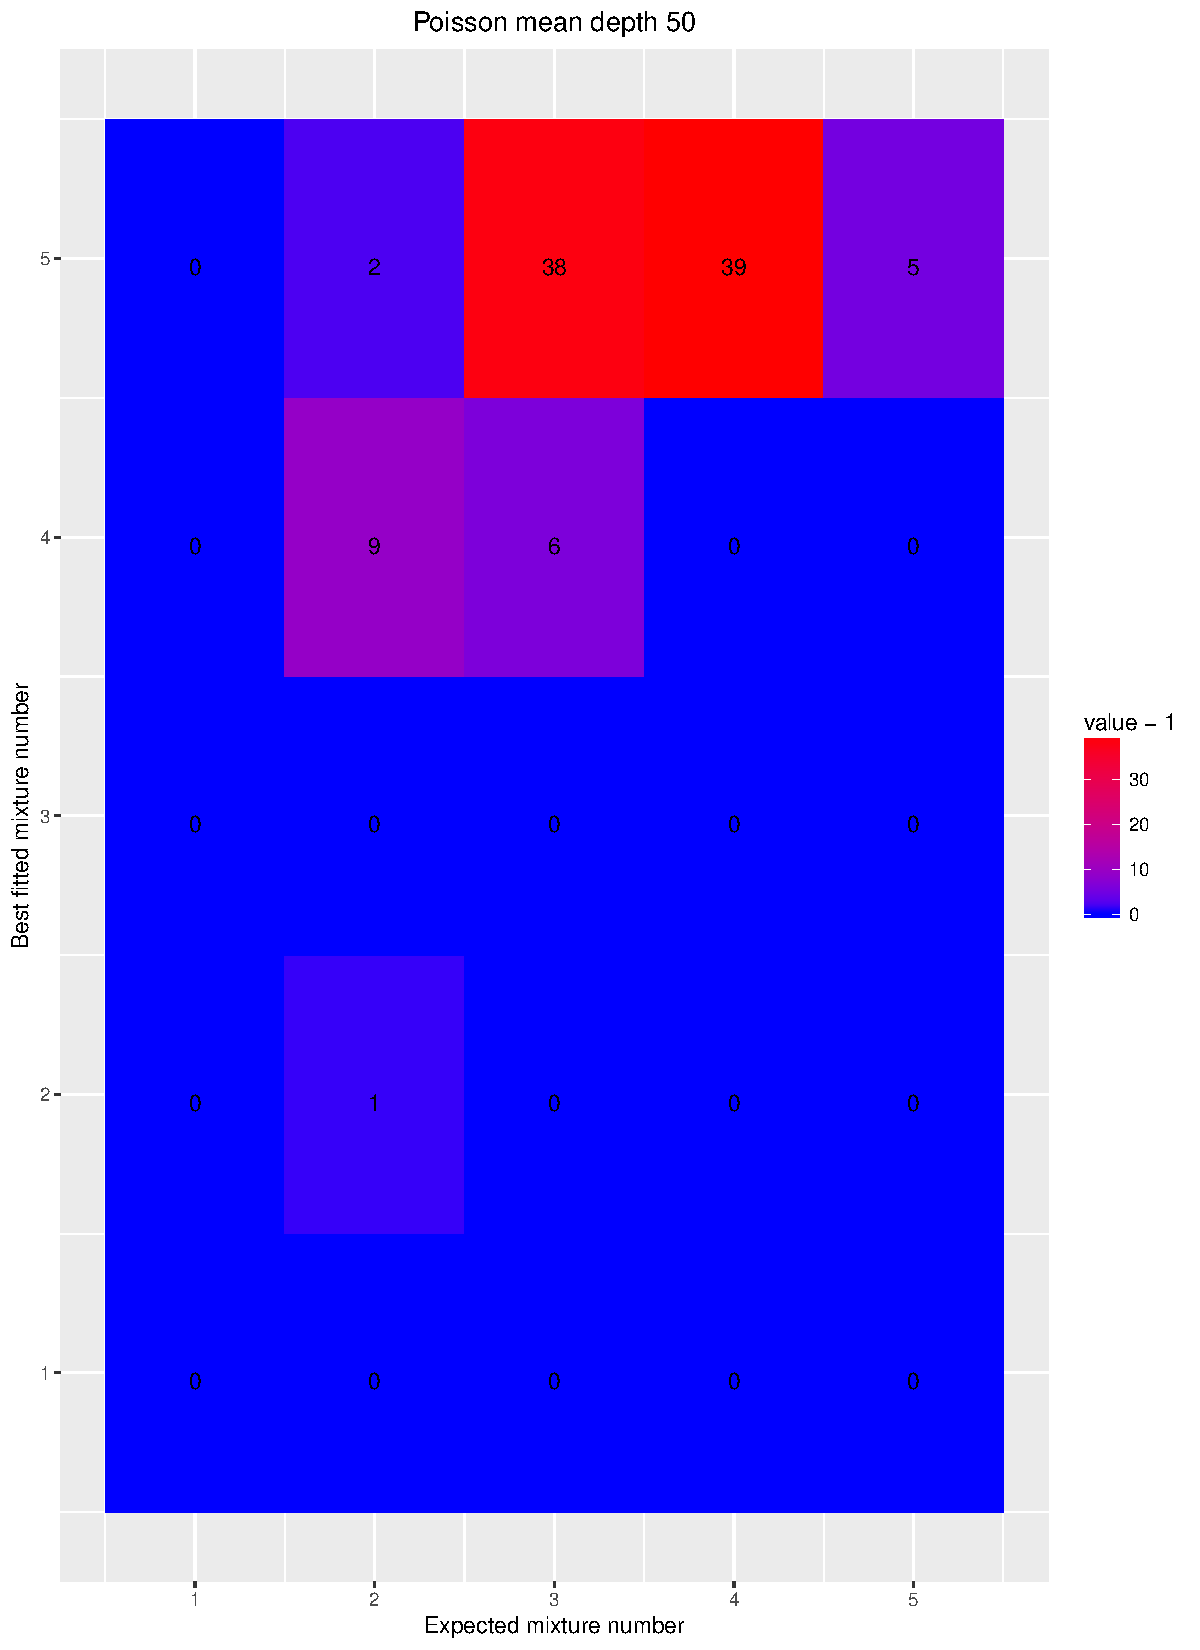
\includegraphics[scale=0.27]{../Results/Third_Analysis/Poisson_Confusion_Matrix_50.pdf}
%\caption{Confusion matrices of the optimal number of curves in the fitted models for the Poisson distribution for 100 genomes at each mean haploid read depth, each generated with random ploidy levels.}
%% Confusion matrices
%\end{center}
%\end{figure}


\begin{table}[H]
\begin{center}
\caption{RMSD for the predicted number of ploidies for models fitted with the optimal number of curves for each distribution. }
\begin{tabular}{|c||P{4cm}|P{4cm}|}
\hline
\multirow{2}{*}{\textbf{MHRD}} & \multicolumn{2}{|c|}{\textbf{RMSD}} \\
\cline{2-3}
& \textbf{Poisson mixture} & \textbf{Negative Binomial mixture} \\
\hline
\hline
\textbf{2} & 1.400 & 1.786 \\
\hline
\textbf{5} & 0.387 & 0.872 \\
\hline
\textbf{10} & 0.663 & 0.490 \\
\hline
\textbf{25} & 1.253 & 0.800 \\
\hline
\textbf{50} & 1.584 & 1.225 \\
\hline
\hline
\end{tabular}
\end{center}
\end{table}


When applied to real world data, the mixture of Poisson distributions performed better for all 22 samples. The level of CCNV detected across the samples varies from two to five which is higher than was hypothesised in the paper the data was sourced from \autocite{Farrer2013}. This is probably due to over-fitting as was observed in the simulated data examples. The samples were sequenced at high haploid read depths (approximately 50x) and thus from the results from the simulated data this over-fitting should be expected. Shown below (Figure 5) is the fitted distributions to one of the samples which was hypothesised to have CCNV where it's genome is predominately tetraploid but with 1-3 chromosomes being triploid. The full set of fitted models along with their parameters can be found in the supplementary materials.  

\begin{figure}[H]
\begin{center}
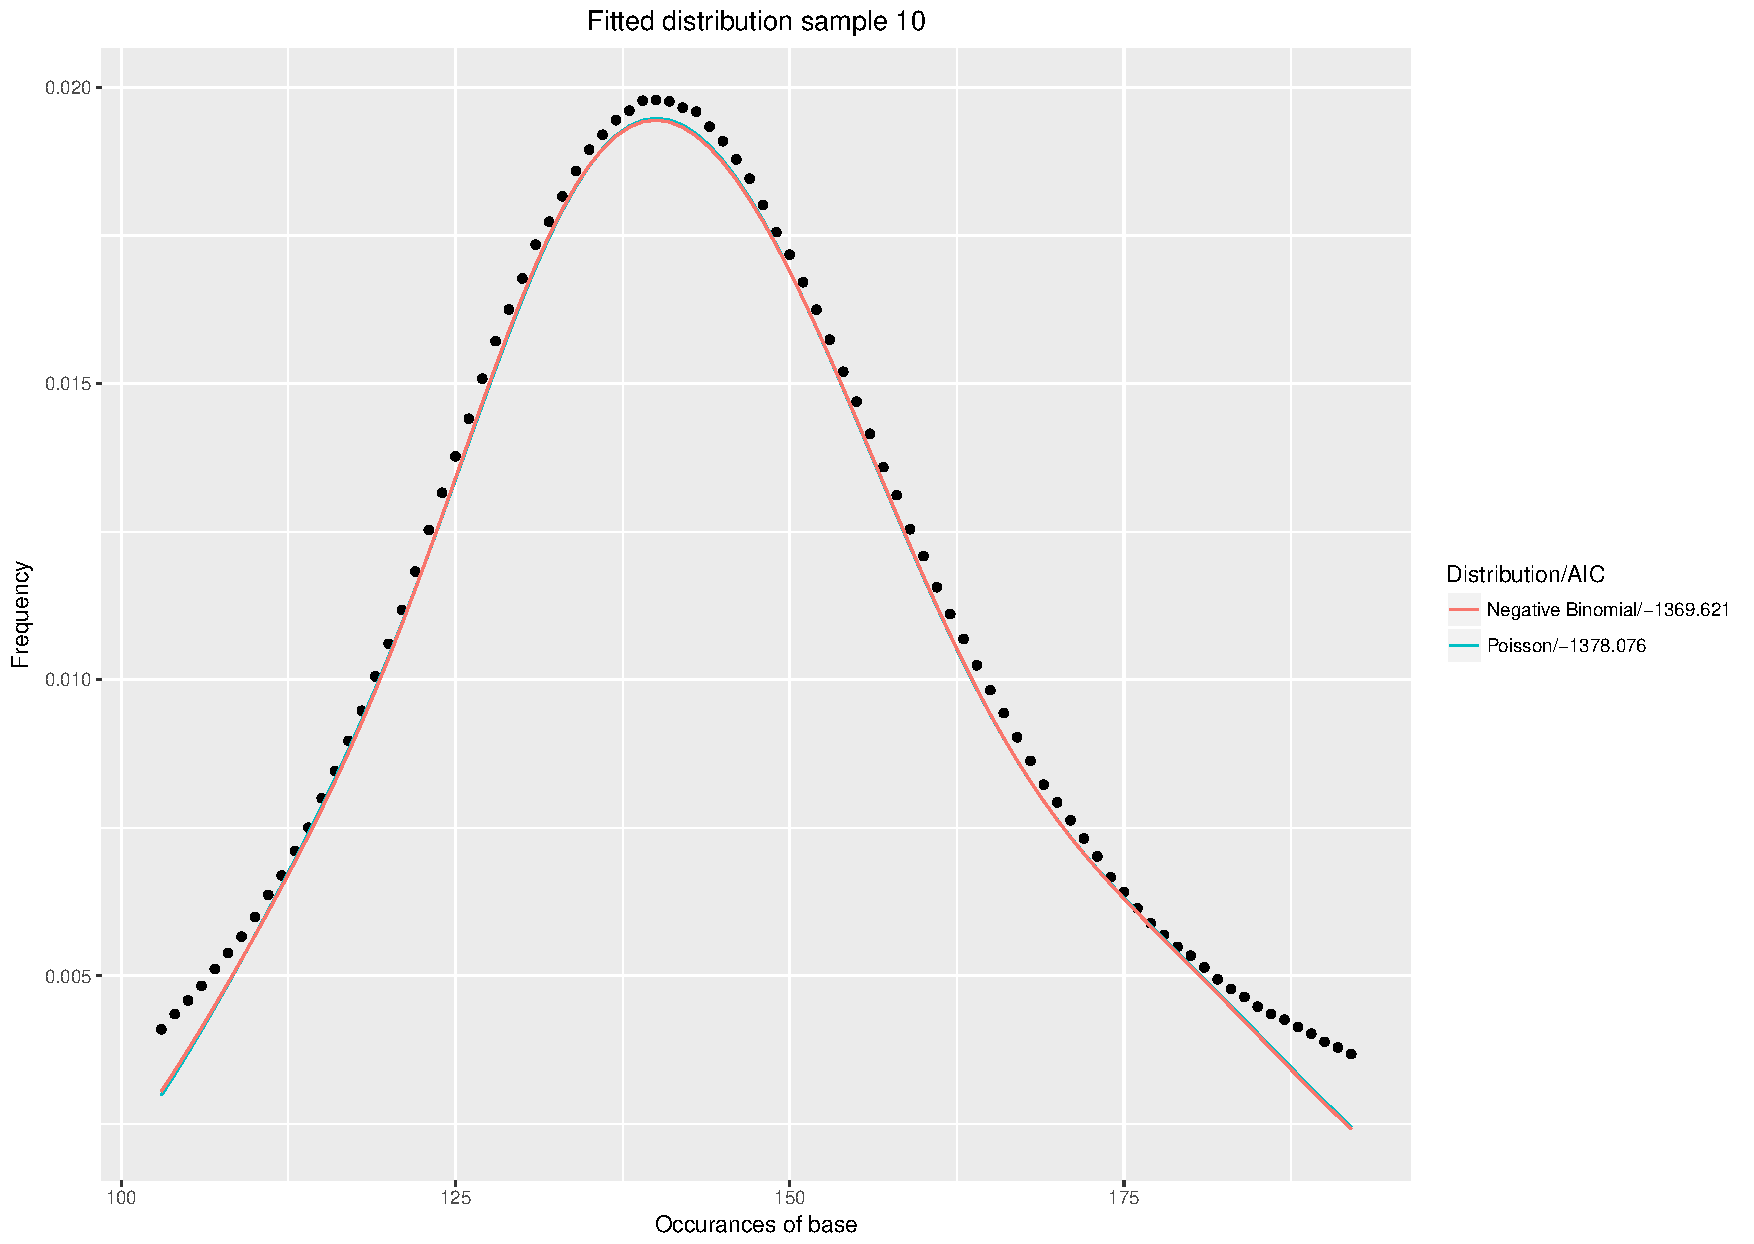
\includegraphics[scale=0.5]{../Results/Bd_Results/10_Supercontig_1_sample_10_plot.pdf}

% Confusion matrices
\end{center}
\caption{Best fitted distributions to the tenth sample (JEL423\textunderscore2014) believed to be tetraploid with triploid chromosomes. Both the optimal mixture of Poisson and Negative Binomial distributions consist of 4 curves.}
\end{figure}

\section{Discussion}
\subsection{Results Analysis}
\paragraph{}Each stage of the analysis has suggested that a singular or mixture of Poisson distributions most accurately models NGS data at low mean haploid read depths but at higher depths the Negative Binomial distribution is better suited. This suggests Negative Binomial is better at modelling the sequencing errors and variation that occur during NGS \autocite{Robasky2014}. When the haploid mean read depth increases, the variation in the data will naturally increase. Variation has a linear relationship with the mean for a Poisson  distribution whilst for the Negative binomial distribution the relationship is exponential (equations 6-8). It appears that the natural increase in variation replicates the exponential behaviour. However, when tested on real world data which had been sequenced at high depths the opposite was observed. In these cases the Poisson distribution proved better at fitting to the datasets contradictory to what was predicted to simulated data. If dealing with real world data which has been sequenced at low depths this difference may not still be observed and the Poisson distribution may still fit better. The main difference observed in the real world data is the amount of variation of read depths observed. These findings suggest that the assumptions used to generate the simulated data may need to be changed to more accurately represent the data observed in the real world. In particular the level of error built into the simulated data may need to be increased to replicate the natural amount of variation found in real datasets.   
\paragraph{}
Poisson: 
\begin{equation}
Mean = \lambda = Variance
\end{equation}
\paragraph{}
Negative Binomial: 
\begin{equation}
Mean = pr/(1-p) = \lambda
\end{equation}
\begin{equation} 
Variance = pr/(1-p)^2 = \lambda + (1/r)\lambda^2
\end{equation} 
\paragraph{}Additional to the incorporation of variance, at all depths, the Negative Binomial distribution demonstrated an increased ability to accurately predict the amount of CCNV in the genome over the Poisson distribution at high read depths, whilst the Poisson remained a stronger predictor at low depths. Both distributions fit better at lower mean haploid read depths and are prone to over-fitting at higher mean haploid read depths but this is more pronounced in the Poisson distribution than the Negative Binomial. Further evidence can be derived from this that the Negative Binomial distribution models the variation in NGS better. Increased variance at higher read depths will give the distribution of data a more negative kurtosis which could allow multiple copies of scaled down distributions to model a curve  for a single ploidy level which should therefore be modelled by a singular distribution. The results above suggest the shape of the tails on the negative binomial distribution provide an appropriate distribution such that this over-fitting becomes considerably less likely. \\  
\paragraph{}A notable change is observed between the RMSD when the genomes have randomly generated CCNV across the genome compared to those generated with stepped ploidy increases. At low depths this is a decrease for the random ploidy genomes and at high depths an increase. At high depths this provides evidence contrary to the assumption that the models would struggle more to differentiate between neighbouring ploidy levels than it would between more distinct peaks. An alternative explanation could be found in investigating the lengths of segments at each ploidy level. In the stepped data the lengths of the chromosomes at each ploidy level were uniform. With randomly assigned ploidy levels to each chromosome many samples had multiple chromosomes at the same ploidy levels, thus the distribution of the genome split between the ploidy levels present was not necessarily uniform. The current initial parameters selection and model fitting technique may not be sufficient to capture this behaviour accurately and could be causing the decrease in accuracy which is experienced. Further analysis of the resulting parameters of the fitted models would be required to determine to what extent this is impacting the results.\\  


\subsection{Opportunities for further study}
\paragraph{}Simulations fitted throughout this study indicate that the Poisson distribution is well suited at modelling the distribution of NGS data at low read depths. They also suggest that the Negative Binomial distribution could potentially be equally well suited for modelling distributions at high read depths with an advantage for predicting the amount of ploidy variation within a genome. However, the parameters of the fitted models have not been analysed to indicate whether the models can accurately predict the actual ploidies present in the genome rather than just how many ploidies exist. \\
\paragraph{}Studies already exist on the extent to which a mixture of Poisson distributions can reduce the error in modelling NGS data and the advantages this brings \autocite{Schwarzbauer2010}. Similar research may lead to intersting results if applied to using the Negative Binomial distribution instead. Also, we can apply a similar EM algorithm to infer ploidy variation of unknown genomes. The findings of which could be applied to real life data sets in order to develop a more accurate understanding of the role of CCNV in various scenarios \autocite{Farrer2013,Yan2017}.\\

\section{Acknowledgements}
\paragraph{}I would like to specially thank Dr. Matteo Fumagalli for his supervision of this project. His provision of assistance and direction throughout the project allowed for the development of ideas and proved invaluable in its completion.
\pagebreak 
\printbibliography
\pagebreak


\section{Supplementary material}
\begin{adjustbox}{angle=90,center,caption={The resulting parameters from fitting mixtures of Poisson distributions to the real world data samples.},nofloat=table}
\begin{tiny}
\csvautotabular{poissondata.csv}
\end{tiny}
\end{adjustbox}
\pagebreak
\begin{adjustbox}{angle=90,center,caption={The resulting parameters from fitting mixtures of Negative Binomial distributions to the real world data samples.},nofloat=table}
\begin{tiny}
\csvautotabular{negativebinomialdata.csv}
\end{tiny}
\end{adjustbox}

\begin{table}[H]
\begin{center}
\caption{Reference names for the samples used in the real world data analysis.}
\begin{tabular}{|c|c|}
\hline
\textbf{Sample Number} & \textbf{Sample Reference} \\
\hline
\hline
Sample 1 & ACON \\
\hline
Sample 2 & AP15 \\
\hline
Sample 3 & APEP \\
\hline
Sample 4 & AUL \\
\hline
Sample 5 & BEW2 \\
\hline
Sample 6 & BLI1 \\
\hline
Sample 7 & CONT.2A.FROZEN \\
\hline
Sample 8 & ETH2 \\
\hline
Sample 9 & ETH4 \\
\hline
Sample 10 & JEL423 \textunderscore 2014 \\
\hline
Sample 11 & MAD \\
\hline
Sample 12 & MG1 \\
\hline
Sample 13 & MG4 \\
\hline
Sample 14 & MODS27.3 \\
\hline
Sample 15 & MODS28 \\
\hline
Sample 16 & RC5.1 \\
\hline
Sample 17 & SA1d \\
\hline
Sample 18 & SA4c \\
\hline
Sample 19 & SFBC014 \\
\hline
Sample 20 & SP10 \\
\hline
Sample 21 & TF5a1 \\
\hline
Sample 22 & VC1 \\
\hline


\end{tabular}
\end{center}
\end{table}


\end{document}
